\documentclass[12pt]{tufte-book}
%DIF LATEXDIFF DIFFERENCE FILE
%DIF DEL old-notes-F24.tex   Sat Sep 21 00:59:03 2024
%DIF ADD notes-F24.tex       Wed Oct  2 20:00:20 2024
\usepackage{amsthm,amssymb,amsmath,thmtools,datetime,tikz}
\setcounter{secnumdepth}{3}

\declaretheorem[numberwithin=chapter,shaded={bgcolor=Lavender}]{definition}

\declaretheorem[numberwithin=chapter,shaded={bgcolor=Thistle}]{lemma}
\declaretheorem[numberwithin=chapter,shaded={bgcolor=Thistle}]{claim}

\declaretheorem[numberwithin=chapter,shaded={bgcolor=Apricot}]{theorem}

\declaretheorem[numberwithin=chapter,shaded={bgcolor=yellow}]{remark}
\declaretheorem[numberwithin=chapter]{exercise}
\declaretheorem[numberwithin=chapter,shaded={bgcolor=pink}]{construction}
\usepackage[
    type={CC},
    modifier={by-nc-nd},
    version={4.0},
]{doclicense}

\usepackage{graphicx,xcolor,mdframed}
%\usepackage[version=0.96]{pgf}
\usepackage{enumitem}

%DIF 25a25
 %DIF > 
%DIF -------
\def\chpcolor{blue!45}
\def\chpcolortxt{blue!60}

\iffalse
\titleformat{\chapter}%
  {\huge\rmfamily\itshape\color{red}}% format applied to label+text
  {\llap{\colorbox{red}{\parbox{1.5cm}{\hfill\itshape\huge\color{white}\thechapter}}}}% label
  {2pt}% horizontal separation between label and title body
  {}% before the title body
  []% after the title body
\fi

\hypersetup{colorlinks}% uncomment this line if you prefer colored hyperlinks (e.g., for onscreen viewing)

%%
% Book metadata
\title{A Course in Theory of Cryptography}
\author[Sanjam Garg]{Sanjam Garg}
%\publisher{Publisher of This Book}

%%
% If they're installed, use Bergamo and Chantilly from www.fontsite.com.
% They're clones of Bembo and Gill Sans, respectively.
%\IfFileExists{bergamo.sty}{\usepackage[osf]{bergamo}}{}% Bembo
%\IfFileExists{chantill.sty}{\usepackage{chantill}}{}% Gill Sans

%\usepackage{microtype}

%%
% Just some sample text
\usepackage{lipsum}
\newcommand{\ma}{\mathcal{A}}
\newcommand{\cA}{\mathcal{A}}
\newcommand{\mb}{\mathcal{B}}
\newcommand{\cB}{\mathcal{B}}

\newcommand{\getsr}{\xleftarrow{\$}}
\newcommand{\bit}{\{0,1\}}

\newcommand{\Gen}{\mathsf{Gen}}
\newcommand{\gen}{\mathsf{Gen}}
\newcommand{\Enc}{\mathsf{Enc}}
% \newcommand{\enc}{\mathsf{Enc}}
\newcommand{\Dec}{\mathsf{Dec}}
% \newcommand{\dec}{\mathsf{Dec}}
% \newcommand{\pk}{\mathsf{pk}}
% \newcommand{\sk}{\mathsf{sk}}

% \newcommand{\concat}[0]{\; || \;}

% \newcommand{\bin}{\{0,1\}}
% \newcommand{\adv}{\mathcal{A}}
% \newcommand{\advb}{\mathcal{B}}
% \newcommand{\advc}{\mathcal{C}}
% \newcommand{\fake}{\mathsf{FAKE}}

\newcommand{\Sign}{\mathsf{Sign}}
\newcommand{\Verify}{\mathsf{Verify}}
%\newcommand{\negl}{\mathsf{negl}}
\newcommand{\abort}{\mathsf{abort}}
\newcommand{\Sampler}{\mathsf{Sampler}}
\newcommand{\Eval}{\mathsf{Eval}}
\renewcommand{\tag}{\mathsf{tag}}
\newcommand{\PRF}{\mathsf{PRF}}

%%
% For nicely typeset tabular material
\usepackage{booktabs}

\usepackage[n,advantage,operators,sets,adversary,landau,probability,notions,logic,ff,mm,primitives,events,complexity,oracles,asymptotics,keys]{cryptocode} 
%%
% For graphics / images
\usepackage{graphicx,algpseudocode}
\setkeys{Gin}{width=\linewidth,totalheight=\textheight,keepaspectratio}
\graphicspath{{graphics/}}

% The fancyvrb package lets us customize the formatting of verbatim
% environments.  We use a slightly smaller font.
\usepackage{fancyvrb}
\fvset{fontsize=\normalsize}

%%
% Prints argument within hanging parentheses (i.e., parentheses that take
% up no horizontal space).  Useful in tabular environments.
\newcommand{\hangp}[1]{\makebox[0pt][r]{(}#1\makebox[0pt][l]{)}}

%%
% Prints an asterisk that takes up no horizontal space.
% Useful in tabular environments.
\newcommand{\hangstar}{\makebox[0pt][l]{*}}

%%
% Prints a trailing space in a smart way.
\usepackage{xspace}

%%
% Some shortcuts for Tufte's book titles.  The lowercase commands will
% produce the initials of the book title in italics.  The all-caps commands
% will print out the full title of the book in italics.
\newcommand{\vdqi}{\textit{VDQI}\xspace}
\newcommand{\ei}{\textit{EI}\xspace}
\newcommand{\ve}{\textit{VE}\xspace}
\newcommand{\be}{\textit{BE}\xspace}
\newcommand{\VDQI}{\textit{The Visual Display of Quantitative Information}\xspace}
\newcommand{\EI}{\textit{Envisioning Information}\xspace}
\newcommand{\VE}{\textit{Visual Explanations}\xspace}
\newcommand{\BE}{\textit{Beautiful Evidence}\xspace}

\newcommand{\TL}{Tufte-\LaTeX\xspace}

% Prints the month name (e.g., January) and the year (e.g., 2008)
\newcommand{\monthyear}{%
  \ifcase\month\or January\or February\or March\or April\or May\or June\or
  July\or August\or September\or October\or November\or
  December\fi\space\number\year
}


% Prints an epigraph and speaker in sans serif, all-caps type.
\newcommand{\openepigraph}[2]{%
  %\sffamily\fontsize{14}{16}\selectfont
  \begin{fullwidth}
  \sffamily\large
  \begin{doublespace}
  \noindent\allcaps{#1}\\% epigraph
  \noindent\allcaps{#2}% author
  \end{doublespace}
  \end{fullwidth}
}

% Inserts a blank page
\newcommand{\blankpage}{\newpage\hbox{}\thispagestyle{empty}\newpage}

\usepackage{units}

% Typesets the font size, leading, and measure in the form of 10/12x26 pc.
\newcommand{\measure}[3]{#1/#2$\times$\unit[#3]{pc}}

% Macros for typesetting the documentation
\newcommand{\hlred}[1]{\textcolor{Maroon}{#1}}% prints in red
\newcommand{\hangleft}[1]{\makebox[0pt][r]{#1}}
\newcommand{\hairsp}{\hspace{1pt}}% hair space
\newcommand{\hquad}{\hskip0.5em\relax}% half quad space
\newcommand{\TODO}{\textcolor{red}{\bf TODO!}\xspace}
\newcommand{\ie}{\textit{i.\hairsp{}e.}\xspace}
\newcommand{\eg}{\textit{e.\hairsp{}g.}\xspace}
\newcommand{\na}{\quad--}% used in tables for N/A cells
\providecommand{\XeLaTeX}{X\lower.5ex\hbox{\kern-0.15em\reflectbox{E}}\kern-0.1em\LaTeX}
\newcommand{\tXeLaTeX}{\XeLaTeX\index{XeLaTeX@\protect\XeLaTeX}}
% \index{\texttt{\textbackslash xyz}@\hangleft{\texttt{\textbackslash}}\texttt{xyz}}
\newcommand{\tuftebs}{\symbol{'134}}% a backslash in tt type in OT1/T1
\newcommand{\doccmdnoindex}[2][]{\texttt{\tuftebs#2}}% command name -- adds backslash automatically (and doesn't add cmd to the index)
\newcommand{\doccmddef}[2][]{%
  \hlred{\texttt{\tuftebs#2}}\label{cmd:#2}%
  \ifthenelse{\isempty{#1}}%
    {% add the command to the index
      \index{#2 command@\protect\hangleft{\texttt{\tuftebs}}\texttt{#2}}% command name
    }%
    {% add the command and package to the index
      \index{#2 command@\protect\hangleft{\texttt{\tuftebs}}\texttt{#2} (\texttt{#1} package)}% command name
      \index{#1 package@\texttt{#1} package}\index{packages!#1@\texttt{#1}}% package name
    }%
}% command name -- adds backslash automatically
\newcommand{\doccmd}[2][]{%
  \texttt{\tuftebs#2}%
  \ifthenelse{\isempty{#1}}%
    {% add the command to the index
      \index{#2 command@\protect\hangleft{\texttt{\tuftebs}}\texttt{#2}}% command name
    }%
    {% add the command and package to the index
      \index{#2 command@\protect\hangleft{\texttt{\tuftebs}}\texttt{#2} (\texttt{#1} package)}% command name
      \index{#1 package@\texttt{#1} package}\index{packages!#1@\texttt{#1}}% package name
    }%
}% command name -- adds backslash automatically
\newcommand{\docopt}[1]{\ensuremath{\langle}\textrm{\textit{#1}}\ensuremath{\rangle}}% optional command argument
\newcommand{\docarg}[1]{\textrm{\textit{#1}}}% (required) command argument
\newenvironment{docspec}{\begin{quotation}\ttfamily\parskip0pt\parindent0pt\ignorespaces}{\end{quotation}}% command specification environment
\newcommand{\docenv}[1]{\texttt{#1}\index{#1 environment@\texttt{#1} environment}\index{environments!#1@\texttt{#1}}}% environment name
\newcommand{\docenvdef}[1]{\hlred{\texttt{#1}}\label{env:#1}\index{#1 environment@\texttt{#1} environment}\index{environments!#1@\texttt{#1}}}% environment name
\newcommand{\docpkg}[1]{\texttt{#1}\index{#1 package@\texttt{#1} package}\index{packages!#1@\texttt{#1}}}% package name
\newcommand{\doccls}[1]{\texttt{#1}}% document class name
\newcommand{\docclsopt}[1]{\texttt{#1}\index{#1 class option@\texttt{#1} class option}\index{class options!#1@\texttt{#1}}}% document class option name
\newcommand{\docclsoptdef}[1]{\hlred{\texttt{#1}}\label{clsopt:#1}\index{#1 class option@\texttt{#1} class option}\index{class options!#1@\texttt{#1}}}% document class option name defined
\newcommand{\docmsg}[2]{\bigskip\begin{fullwidth}\noindent\ttfamily#1\end{fullwidth}\medskip\par\noindent#2}
\newcommand{\docfilehook}[2]{\texttt{#1}\index{file hooks!#2}\index{#1@\texttt{#1}}}
\newcommand{\doccounter}[1]{\texttt{#1}\index{#1 counter@\texttt{#1} counter}}

% Generates the index
\usepackage{makeidx}
\makeindex
%DIF PREAMBLE EXTENSION ADDED BY LATEXDIFF
%DIF UNDERLINE PREAMBLE %DIF PREAMBLE
\RequirePackage[normalem]{ulem} %DIF PREAMBLE
\RequirePackage{color}\definecolor{RED}{rgb}{1,0,0}\definecolor{BLUE}{rgb}{0,0,1} %DIF PREAMBLE
\providecommand{\DIFadd}[1]{{\protect\color{blue}\uwave{#1}}} %DIF PREAMBLE
\providecommand{\DIFdel}[1]{{\protect\color{red}\sout{#1}}}                      %DIF PREAMBLE
%DIF SAFE PREAMBLE %DIF PREAMBLE
\providecommand{\DIFaddbegin}{} %DIF PREAMBLE
\providecommand{\DIFaddend}{} %DIF PREAMBLE
\providecommand{\DIFdelbegin}{} %DIF PREAMBLE
\providecommand{\DIFdelend}{} %DIF PREAMBLE
\providecommand{\DIFmodbegin}{} %DIF PREAMBLE
\providecommand{\DIFmodend}{} %DIF PREAMBLE
%DIF FLOATSAFE PREAMBLE %DIF PREAMBLE
\providecommand{\DIFaddFL}[1]{\DIFadd{#1}} %DIF PREAMBLE
\providecommand{\DIFdelFL}[1]{\DIFdel{#1}} %DIF PREAMBLE
\providecommand{\DIFaddbeginFL}{} %DIF PREAMBLE
\providecommand{\DIFaddendFL}{} %DIF PREAMBLE
\providecommand{\DIFdelbeginFL}{} %DIF PREAMBLE
\providecommand{\DIFdelendFL}{} %DIF PREAMBLE
\newcommand{\DIFscaledelfig}{0.5}
%DIF HIGHLIGHTGRAPHICS PREAMBLE %DIF PREAMBLE
\RequirePackage{settobox} %DIF PREAMBLE
\RequirePackage{letltxmacro} %DIF PREAMBLE
\newsavebox{\DIFdelgraphicsbox} %DIF PREAMBLE
\newlength{\DIFdelgraphicswidth} %DIF PREAMBLE
\newlength{\DIFdelgraphicsheight} %DIF PREAMBLE
% store original definition of \includegraphics %DIF PREAMBLE
\LetLtxMacro{\DIFOincludegraphics}{\includegraphics} %DIF PREAMBLE
\newcommand{\DIFaddincludegraphics}[2][]{{\color{blue}\fbox{\DIFOincludegraphics[#1]{#2}}}} %DIF PREAMBLE
\newcommand{\DIFdelincludegraphics}[2][]{% %DIF PREAMBLE
\sbox{\DIFdelgraphicsbox}{\DIFOincludegraphics[#1]{#2}}% %DIF PREAMBLE
\settoboxwidth{\DIFdelgraphicswidth}{\DIFdelgraphicsbox} %DIF PREAMBLE
\settoboxtotalheight{\DIFdelgraphicsheight}{\DIFdelgraphicsbox} %DIF PREAMBLE
\scalebox{\DIFscaledelfig}{% %DIF PREAMBLE
\parbox[b]{\DIFdelgraphicswidth}{\usebox{\DIFdelgraphicsbox}\\[-\baselineskip] \rule{\DIFdelgraphicswidth}{0em}}\llap{\resizebox{\DIFdelgraphicswidth}{\DIFdelgraphicsheight}{% %DIF PREAMBLE
\setlength{\unitlength}{\DIFdelgraphicswidth}% %DIF PREAMBLE
\begin{picture}(1,1)% %DIF PREAMBLE
\thicklines\linethickness{2pt} %DIF PREAMBLE
{\color[rgb]{1,0,0}\put(0,0){\framebox(1,1){}}}% %DIF PREAMBLE
{\color[rgb]{1,0,0}\put(0,0){\line( 1,1){1}}}% %DIF PREAMBLE
{\color[rgb]{1,0,0}\put(0,1){\line(1,-1){1}}}% %DIF PREAMBLE
\end{picture}% %DIF PREAMBLE
}\hspace*{3pt}}} %DIF PREAMBLE
} %DIF PREAMBLE
\LetLtxMacro{\DIFOaddbegin}{\DIFaddbegin} %DIF PREAMBLE
\LetLtxMacro{\DIFOaddend}{\DIFaddend} %DIF PREAMBLE
\LetLtxMacro{\DIFOdelbegin}{\DIFdelbegin} %DIF PREAMBLE
\LetLtxMacro{\DIFOdelend}{\DIFdelend} %DIF PREAMBLE
\DeclareRobustCommand{\DIFaddbegin}{\DIFOaddbegin \let\includegraphics\DIFaddincludegraphics} %DIF PREAMBLE
\DeclareRobustCommand{\DIFaddend}{\DIFOaddend \let\includegraphics\DIFOincludegraphics} %DIF PREAMBLE
\DeclareRobustCommand{\DIFdelbegin}{\DIFOdelbegin \let\includegraphics\DIFdelincludegraphics} %DIF PREAMBLE
\DeclareRobustCommand{\DIFdelend}{\DIFOaddend \let\includegraphics\DIFOincludegraphics} %DIF PREAMBLE
\LetLtxMacro{\DIFOaddbeginFL}{\DIFaddbeginFL} %DIF PREAMBLE
\LetLtxMacro{\DIFOaddendFL}{\DIFaddendFL} %DIF PREAMBLE
\LetLtxMacro{\DIFOdelbeginFL}{\DIFdelbeginFL} %DIF PREAMBLE
\LetLtxMacro{\DIFOdelendFL}{\DIFdelendFL} %DIF PREAMBLE
\DeclareRobustCommand{\DIFaddbeginFL}{\DIFOaddbeginFL \let\includegraphics\DIFaddincludegraphics} %DIF PREAMBLE
\DeclareRobustCommand{\DIFaddendFL}{\DIFOaddendFL \let\includegraphics\DIFOincludegraphics} %DIF PREAMBLE
\DeclareRobustCommand{\DIFdelbeginFL}{\DIFOdelbeginFL \let\includegraphics\DIFdelincludegraphics} %DIF PREAMBLE
\DeclareRobustCommand{\DIFdelendFL}{\DIFOaddendFL \let\includegraphics\DIFOincludegraphics} %DIF PREAMBLE
%DIF COLORLISTINGS PREAMBLE %DIF PREAMBLE
\RequirePackage{listings} %DIF PREAMBLE
\RequirePackage{color} %DIF PREAMBLE
\lstdefinelanguage{DIFcode}{ %DIF PREAMBLE
%DIF DIFCODE_UNDERLINE %DIF PREAMBLE
  moredelim=[il][\color{red}\sout]{\%DIF\ <\ }, %DIF PREAMBLE
  moredelim=[il][\color{blue}\uwave]{\%DIF\ >\ } %DIF PREAMBLE
} %DIF PREAMBLE
\lstdefinestyle{DIFverbatimstyle}{ %DIF PREAMBLE
	language=DIFcode, %DIF PREAMBLE
	basicstyle=\ttfamily, %DIF PREAMBLE
	columns=fullflexible, %DIF PREAMBLE
	keepspaces=true %DIF PREAMBLE
} %DIF PREAMBLE
\lstnewenvironment{DIFverbatim}{\lstset{style=DIFverbatimstyle}}{} %DIF PREAMBLE
\lstnewenvironment{DIFverbatim*}{\lstset{style=DIFverbatimstyle,showspaces=true}}{} %DIF PREAMBLE
%DIF END PREAMBLE EXTENSION ADDED BY LATEXDIFF

\begin{document}
\iffalse
% Front matter
\frontmatter

% r.1 blank page
\blankpage


% v.2 epigraphs
\newpage\thispagestyle{empty}
\openepigraph{%
The public is more familiar with bad design than good design.
It is, in effect, conditioned to prefer bad design, 
because that is what it lives with. 
The new becomes threatening, the old reassuring.
}{Paul Rand%, {\itshape Design, Form, and Chaos}
}
\vfill
\openepigraph{%
A designer knows that he has achieved perfection 
not when there is nothing left to add, 
but when there is nothing left to take away.
}{Antoine de Saint-Exup\'{e}ry}
\vfill
\openepigraph{%
\ldots the designer of a new system must not only be the implementor and the first 
large-scale user; the designer should also write the first user manual\ldots 
If I had not participated fully in all these activities, 
literally hundreds of improvements would never have been made, 
because I would never have thought of them or perceived 
why they were important.
}{Donald E. Knuth}
\fi

% r.3 full title page
\maketitle


% v.4 copyright page
%\newpage
\begin{fullwidth}
~\vfill
\thispagestyle{empty}
\setlength{\parindent}{0pt}
\setlength{\parskip}{\baselineskip}
Copyright \copyright\ \the\year\ \thanklessauthor

%\par\smallcaps{Published by \thanklesspublisher}

\par\smallcaps{This document is continually being updated. Please send us your feedback.}


\par \doclicenseThis
 \index{license}

\par\textit{This draft was compiled on \today.}
\end{fullwidth}

% r.5 contents
\tableofcontents

%\listoffigures

%\listoftables

% r.7 dedication
\iffalse
\cleardoublepage
~\vfill

\begin{doublespace}
\noindent\fontsize{18}{22}\selectfont\itshape
\nohyphenation
Dedicated to those who appreciate \LaTeX{} 
and the work of \mbox{Edward R.~Tufte} 
and \mbox{Donald E.~Knuth}.
\end{doublespace}
\vfill
\vfill

% r.9 introduction
\cleardoublepage
\fi
\chapter*{Preface}
Cryptography enables many paradoxical objects, such as public key encryption, verifiable electronic signatures, zero-knowledge protocols, and fully homomorphic encryption.  The two main steps in developing such seemingly impossible primitives are (i) defining the desired security properties formally and (ii) obtaining a construction satisfying the security property provably. In modern cryptography, the second step typically assumes (unproven) computational assumptions, which are conjectured to be computationally intractable. In this course, we will define several cryptographic primitives and argue their security based on well-studied computational hardness assumptions. However, we will largely ignore the mathematics underlying the assumed computational intractability assumptions.

\section*{Acknowledgements}
These lecture notes are based on scribe notes taken by students in CS 276 over the years. Also, thanks to Peihan Miao, Akshayaram Srinivasan, and Bhaskar Roberts for helping to improve these notes.
%%
% Start the main matter (normal chapters)
\newcommand{\sanjam}[1]{{\color{red} Sanjam: #1}}

\newcommand{\bhaskar}[1]{{\color{ForestGreen} Bhaskar: #1}}


\mainmatter
\chapter{Mathematical Background}
\label{sec:mb}

In modern cryptography, (1) we typically assume that our attackers cannot run in unreasonably large amounts of time, and (2) we allow security to be broken with a \emph{very small}, but non-zero, probability.

Without these assumptions, we must work in the realm of information-theoretic cryptography, which is often unachievable or impractical for many applications. For example, the one-time pad
\footnote{For a message $m \in \{0,1\}^n$ and a random key $k \in \{0,1\}^n$, the encryption of $m$ is $c = m \oplus k$. The decryption is $m = c \oplus k$.}
-- an information-theoretically secure cipher -- is not very useful because it requires very large keys.

In this chapter, we define items (1) and (2) more formally. We require our adversaries to run in polynomial time, which captures the idea that their runtime is not unreasonably large (sections~\ref{ssec:ppt}). We also allow security to be broken with negligible -- very small -- probability (section ~\ref{ssec:nnf}). 


\section{Probabilistic Polynomial Time}
\label{ssec:ppt}
A probabilistic Turing Machine is a generic computer that is allowed to make random choices during its execution. A probabilistic \textit{polynomial time} Turing Machine is one which halts in time polynomial in its input length. More formally:

\begin{definition}[Probabilistic Polynomial Time]
A probabilistic Turing Machine $M$ is said to be PPT (a Probabilistic Polynomial Time Turing Machine) if $\exists c \in \mathbb{Z}^+$ such that $\forall x \in\{0,1\}^*$, $M(x)$ halts in $|x|^c$ steps.
\end{definition}

A {\em non-uniform} PPT Turing Machine is a collection of machines one for each input length, as opposed to a single machine that must work for all input lengths.

\begin{definition}[Non-uniform PPT]
A non-uniform PPT machine is a sequence of Turing Machines $\{ M_1, M_2, \cdots \}$ such that $\exists c \in \mathbb{Z}^+$ such that $\forall x \in\{0,1\}^*$, $M_{|x|}(x)$ halts in $|x|^c$ steps.
\end{definition}



\section{Noticeable and Negligible Functions}
\label{ssec:nnf}
Noticeable and negligible functions are used to characterize the ``largeness'' or ``smallness'' of a function describing the probability of some event.  Intuitively, a noticeable function is required to be larger than some inverse-polynomially function in the input parameter. On the other hand, a negligible function must be smaller than any inverse-polynomial function of the input parameter. More formally:


\begin{definition}[Noticeable Function]
A function $\mu(\cdot): \mathbb{Z}^+ \rightarrow [0,1]$ is noticeable iff $\exists c \in \mathbb{Z}^+, n_0 \in \mathbb{Z}^+$ such that $\forall n \geq n_0 , \; \mu(n) > n^{-c}$.
\end{definition}

\paragraph{Example.} Observe that $\mu(n) = n^{-3}$ is a noticeable function.  (Notice that the above definition is satisfied for $c = 4$ and $n_0 = 1$.)

\begin{definition}[Negligible Function]
A function $\mu(\cdot): \mathbb{Z}^+ \rightarrow [0,1]$ is negligible iff $\forall c \in \mathbb{Z}^+ \; \exists n_0 \in \mathbb{Z}^+$ such that $\forall n \geq n_0 , \; \mu(n) < n^{-c}$.
\end{definition}

\paragraph{Example.} $\mu(n) = 2^{-n}$ is an example of a negligible function. This can be observed as follows.
Consider an arbitrary $c \in \mathbb{Z}^+$ and set $n_0 = c^2$. Now, observe that for all $n \geq n_0$, we have that $\frac{n}{\log_2 n} \geq \frac{n_0}{\log_2 n_0} > \frac{n_0}{\sqrt{n_0}} = \sqrt{n_0} = c$. This allows us to conclude that $$\mu(n) = 2^{-n} = n^{-\frac{n}{\log_2 n}} < n^{-c}.$$

Thus, we have proved that for any $c \in \mathbb{Z}^+$, there exists $n_0 \in \mathbb{Z}^+$ such that for any $n \geq n_0$, $\mu(n) < n^{-c}$.

\paragraph{Gap between Noticeable and Negligible Functions.}
At first thought it might seem that a function that is {not} negligible (or, a non-negligible function) must be a noticeable. This is not true!\cite{JC:Bellare02} Negating the definition of a negligible function, we obtain that a non-negligible function $\mu(\cdot)$ is such that $\exists c \in \mathbb{Z}^+$ such that $\forall n_0 \in \mathbb{Z}^+$, $\exists n \geq n_0$ such that $\mu(n) > n^{-c}$.
Note that this requirement is satisfied as long as $\mu(n) > n^{-c}$ for infinitely many choices of $n \in \mathbb{Z}^+$. However, a noticeable function requires this condition to be true for every $n \geq n_0$.

Below we give example of a function $\mu(\cdot)$ that is neither negligible nor noticeable.
$$\mu(n) = \Big\{
\begin{array}{ll}
  2^{-n} & : x \mod 2 = 0\\
  n^{-3} & : x \mod 2 \neq 0
\end{array}
$$
This function is obtained by interleaving negligible and  noticeable functions. It cannot be negligible (resp., noticeable) because it is greater (resp., less) than an inverse-polynomially function for infinitely many input choices.

\paragraph{Properties of Negligible Functions.} Sum and product of two negligible functions is still a negligible function. We argue this for the sum function below and defer the problem for products to Exercise~\ref{ex:product}. These properties together imply that any polynomial function of a negligible function is still negligible.

\begin{exercise}
If $\mu(n)$ and $\nu(n)$ are negligible functions from domain $\mathbb{Z}^+$ to range $[0,1]$ then prove that the following functions are also negligible:
\begin{enumerate}
    \item $\psi_1(n) = \frac{1}{2} \cdot \left(\mu(n) + \nu(n)\right)$
    \item $\psi_2(n) = \min\{\mu(n) + \nu(n), 1\}$
    \item $\psi_3(n) = \mu(n)\cdot \nu(n)$
    \item $\psi_4(n) = \mathsf{poly}(\mu(n))$, where $\mathsf{poly}(\cdot)$ is an unspecified polynomial function. (Assume that the output is also clamped to $[0,1]$ to satisfy the definition)
\end{enumerate}function.
\end{exercise}
\proof 
$ $
\begin{enumerate}
    \item We need to show that for any $c \in \mathbb{Z}^+$, we can find $n_0$ such that $\forall n \geq n_0$, $\psi_1(n) \leq n^{-c}$. Our argument proceeds as follows. Given the fact that $\mu$ and $\nu$ are negligible we can conclude that there exist $n_1$ and $n_2$ such that $\forall n \geq n_1$, $\mu(n) < n^{-c}$ and $\forall n \geq n_2$, $g(n) < n^{-c}$. Combining the above two facts and setting $n_0 = \max(n_1, n_2)$ we have that for every $n \geq n_0$,
    \begin{align*}
        \psi_1(n) &= \frac{1}{2} \cdot (\mu(n) + \nu(n)) < \frac{1}{2} \cdot (n^{-c} + n^{-c}) = n^{-c}
    \end{align*}
    Thus, $\psi_1(n) \leq n^{-c}$ and hence is negligible.

    \item We need to show that for any $c \in \mathbb{Z}^+$, we can find $n_0$ such that $\forall n \geq n_0$, $\psi_2(n) \leq n^{-c}$. Given the fact that $\mu$ and $\nu$ are negligible, there exist $n_1$ and $n_2$ such that $\forall n \geq n_1$, $\mu(n) \leq n^{-c-1}$ and $\forall n \geq n_2$, $g(n) \leq n^{-c-1}$. Setting $n_0 = \max(n_1, n_2, 3)$ we have that for every $n \geq n_0$,
    \begin{align*}
        \psi_2(n) &= \min\{\mu(n) + \nu(n), 1\} < n^{-c-1} + n^{-c-1} < n^{-c}
    \end{align*}
\end{enumerate}
\qed

%\begin{corollary}
%If $f(n)$ is non-negligible and $g(n)$ is negligible, then $h(n) = f(n) - g(n)$ is non-negligible.
%\end{corollary}
%
%\proof If $h(n)$ was negligible, then $f(n) = g(n) + h(n)$ would be the sum of two negligible functions, but would be non-negligible, which is a contradiction.  \qed

\section{Computationally  Hard Problems}\label{sec:assumptions}
%So far, much of our investigation relied on the existence of one-way-functions or in certain cases on the existence of one-one one-way functions. However, just the mere existence of an object is not enough for real-world implementations. 
We will next provide certain number theoretical problems that are conjectured to be computationally intractable. We will use the conjectured hardness of these problems in subsequent chapters to o provide concrete instantiations.

\subsection{The Discrete-Log Family of Problem}
Consider a group $\mathbb{G}$ of prime order. For example, consider the group $\mathbb{Z}_p^*$ where $p$ is a large prime. Let $g$ be a generator of this group $\mathbb{G}$. In this group, given $g^x$ for a random $x \in \{1,\ldots p-1\}$ consider the problem of finding $x$. This problem, referred to as the discrete-log problem, is believed to be computationally hard.

The asymptotic definition of the discrete-log problem needs to consider an infinite family of groups or what we will a group ensemble. 

\paragraph{Group Ensemble.} A group ensemble is a set of finite cyclic groups $\mathcal{G} =\{ \mathbb{G}_n\}_{n \in \mathbb{N}}$. For the group $G_n$, we assume that given two group elements in $G_n$, their sum can be computed in polynomial in $n$ time. Additionally, we assume that given $n$ the generator $g$ of $\mathbb{G}_n$ can be computed in polynomial time. 

\begin{definition}[Discrete-Log Assumption]\label{def:dl}
We say that the discrete-log assumption holds for the group ensemble $\mathcal{G} =\{ \mathbb{G}_n\}_{n \in \mathbb{N}}$, if for every non-uniform PPT algorithm $\mathcal{A}$ we have that
\[\mu_\mathcal{A}(n) := \Pr_{x \leftarrow |G_n|}[\mathcal{A}(g,g^x) = x]\]
is a negligible function.
\end{definition}

\paragraph{The Diffie-Hellman Problems.} In addition to the discrete-log assumption, we also define the Computational Diffie-Hellman Assumption and the Decisional Diffie-Hellman Assumption. 

\begin{definition}[Computational Diffie-Hellman (CDH) Assumption]\label{def:cdh}
We say that the Computational Diffie-Hellman Assumption holds for the group ensemble $\mathcal{G} =\{ \mathbb{G}_n\}_{n \in \mathbb{N}}$, if for every non-uniform PPT algorithm $\mathcal{A}$ we have that
\[\mu_\mathcal{A}(n) := \Pr_{x,y \leftarrow |G_n|}[\mathcal{A}(g,g^x,g^y) = g^{xy}]\]
is a negligible function.
\end{definition}

\begin{definition}[Decisional Diffie-Hellman (DDH) Assumption]\label{def:ddh}
We say that the Computational Diffie-Hellman Assumption holds for the group ensemble $\mathcal{G} =\{ \mathbb{G}_n\}_{n \in \mathbb{N}}$, if for every non-uniform PPT algorithm $\mathcal{A}$ we have that
\[\mu_\mathcal{A}(n) = \mid\Pr_{x,y \leftarrow |G_n|}[\mathcal{A}(g,g^x,g^y,g^{xy}) = 1] - \Pr_{x,y,z \leftarrow |G_n|}[\mathcal{A}(g,g^x,g^y,g^{z}) = 1]\mid\]
is a negligible function.
\end{definition}

It is not hard to observe that the discrete-log assumption is the weakest of the three assumptions above. In fact, it is not difficult to show that the Discrete-Log Assumption for $\mathcal{G}$ implies the CDH and the DDH Assumptions for $\mathcal{G}$.  Additionally, we leave it as an exercise to show that the CDH Assumption for $\mathcal{G}$ implies the  DDH Assumptions for $\mathcal{G}$.

\paragraph{Examples of Groups where these assumptions hold.} Now we provide some examples of group where these assumptions hold. 
\begin{enumerate}
    \item Consider the group $\mathbb{Z}_p^*$ for a prime $p$.\footnote{Since the number of primes is infinite we can define an infinite family of such groups. For the sake of simplicity, here we only consider a single group.} For this group the CDH Assumption is conjectured to be true. However, using the Legendre symbol,\footnote{Let $p$ be an odd prime number. An integer $a$ is said to be a \emph{quadratic residue} modulo $p$ if it is congruent to a perfect square modulo $p$ and  is said to be a \emph{quadratic non-residue} modulo $p$ otherwise. The \emph{Legendre symbol} is a function of $a$ and $p$ defined as
    \begin{equation*}
        \left(\frac{a}{p}\right) = \begin{cases}
    1 &\text{if $a$ is quadration residue mod $p $ and $a \not\equiv 0 \mod p$}\\
    -1 &\text{if $a$ is quadration non-residue mod $p $}\\
    0 &\text{if $a \equiv 0 \mod p $}
    \end{cases}
    \end{equation*}

Legendre symbol can be efficiently computed as $\left(\frac{a}{p}\right) = a^{\frac{p-1}{2}}\mod p$.} 
the DDH Assumption in this group can be shown to be false. Can you show how?\footnote{This is because given $g^x, g^y$ one can easily compute deduce the Legendre symbol of $g^{xy}$.  Observe that if $\left(\frac{g}{p}\right) = -1$ then we have that $\left(\frac{g^{xy}}{p}\right) = 1$ if and only if $ \left(\frac{g^x}{p}\right) =1 $ or $\left(\frac{g^y}{p}\right) = 1$. Using this fact, we can construct an adversary that breaks the DDH problem with a non-negligible (in fact, noticeable) probability.}
\item Let $p = 2q+1$ where both $p$ and $q$ are prime.\footnote{By Dirichet's Theorem on primes in arithmetic progression, we have that there are infinite choices of primes $(p,q)$ for which $p = 2q+1$. This allows us to generalize this group to a group ensemble.} Next, let $\mathbb{Q}$ be the order-$q$ subgroup of quadratic residues in $\mathbb{Z}^*_p$. For this group, the DDH assumption is believed to hold. 
\item Let $N = pq$ where $p,q, \frac{p-1}{2}$ and $\frac{q-1}{2}$ are primes. Let $\mathbb{QR}_N$ be the cyclic subgroup of qudratic resides of order $\phi(N) = (p-1)(q-1)$. For this group $\mathbb{QR}_N$, the DDH assumption is also believed to hold.
%\item Pairings:
\end{enumerate}

\paragraph{Is DDH strictly stronger than Discrete-Log?} In the example cases above, where DDH is known believed to be hard, the
best known algorithms for DDH are no better than the best known algorithms for the discrete-log problem. Whether the DDH assumption is strictly stronger than the discrete-log assumption is an open problem. 



\subsection{CDH in $\mathbb{QR}_N$ implies Factoring}

In this section, we will show that the CDH assumption in $\mathbb{QR}_N$ implies the factoring assumption. 
\begin{lemma}
Given an algorithm $\mathcal{A}$ that breaks the CDH assumption in $\mathbb{QR}_N$, we construct an non-uniform PPT adversary $\mathcal{B}$ that on input $N$ outputs its prime factors $p$ and $q$.
\end{lemma}
\begin{proof}
Given that $\mathcal{A}$ is an algorithm that solves the CDH problem in $\mathbb{QR}_N$ with a non-negligible probability, we construct an algorithm $\mathcal{B}$ that can factor $N$. Specifically, $\mathcal{B}$ on input $N$ proceeds as follows:
\begin{enumerate}
\item Sample $v \leftarrow \mathbb{QR}_N$ (such a $v$ can be obtained by sampling a random value in $\mathbb{Z}_N^*$ and squaring it) and compute $g := v^2 \mod N$.
\item Sample $x, y \leftarrow [N]$.\footnote{Note that sampling $x,y$ uniformly from $[N]$ is statistically close to sampling $x,y$ uniformly from $[\phi(N)]$.}
\item Let $ u := \mathcal{A}(g, g^{x}\cdot v, g^y\cdot v)$\footnote{Note that $g^x\cdot v$ where $x \leftarrow [N]$ is statistically close to $g^x$ where $x \leftarrow [N]$.} and compute $w := \frac{u}{g^{xy}\cdot v^{x+y}}$.
\item If $w^2 = v^2 \mod N$ and $u \neq \pm v$, then compute the factors of $N$ as $\mathsf{gcd}(N,u+v)$ and $N/\mathsf{gcd}(N,u+v)$. Otherwise, output $\bot$.
\end{enumerate}
Observe that if $\mathcal{A}$ solves the CDH problem then the returned values $u = g^{(x+ 2^{-1})(y + 2^{-1})} = v^{2xy + x+ y + 2^{-1}}$. Consequently, the computed value $w = v^{2^{-1}}$. Furthermore, with probability $\frac{1}{2}$ we have that $w \neq v$. In this case, $\mathcal{B}$ can factor $N$.
\end{proof}
\newcommand{\binset}[1]{\{0,1\}^{#1}}
\newcommand{\binfunc}[2]{\binset{#1}\rightarrow\binset{#2}}
%\newcommand{\bin}{\{0,1\}}
%\newcommand{\adv}{\mathcal{A}}
\newcommand{\advb}{\mathcal{B}}
\newcommand{\advc}{\mathcal{C}}

\chapter{One-Way Functions}
\label{sec:owf}

\label{ssec:owf}
Cryptographers often attempt to base cryptographic results on conjectured computational assumptions to leverage reduced adversarial capabilities. Furthermore, the security of these constructions is no better than the assumptions they are based on. 
\begin{quote}
\emph{Cryptographers seldom sleep well.}\footnote{Quote by Silvio Micali in personal communication with Joe Kilian.}
\end{quote}
Thus, basing cryptographic tasks on the \emph{minimal} necessary assumptions is a key tenet in cryptography. Towards this goal, rather can making assumptions about specific computational problem in number theory, cryptographers often consider \emph{abstract primitives}. The existence of these abstract primitives can then be based on one or more computational problems in number theory.

The weakest abstract primitive cryptographers consider is one-way functions. Virtually, every cryptographic goal of interest is known to imply the existence of one-way functions. In other words, most cryptographic tasks would be impossible if the existence of one-way functions was ruled out. On the flip side, the realizing cryptographic tasks from just one-way functions would be ideal. 

\section{Definition}
A one-way function $f: \{0,1\}^n \rightarrow \{0,1\}^m$ is a function that is easy to compute but hard to invert. This intuitive notion is trickier to formalize than it might appear on first thought.

\begin{definition}[One-Way Functions]
A function $f : \binset{*} \rightarrow \binset{*}$ is said to be one-way function if:
\begin{itemize}
\item[-] \textbf{Easy to Compute:} $\exists$ a (deterministic) polynomial time machine $M$ such that $\forall x \in \binset{*}$ we have that \[M(x) = f(x)\]

\item[-] \textbf{Hard to Invert:} $\forall$ non-uniform PPT adversary $\mathcal{A}$ we have that
    \begin{equation}\label{eq:owf}
    \mu_{\mathcal{A},f}(n) = \Pr_{x \stackrel{\$}{\leftarrow} \binset{n}}[ \mathcal{A}(1^n, f(x)) \in f^{-1}(f(x))]
     \end{equation}
     is a negligible function,  $x \overset{\$}{\leftarrow} \binset{n}$ denotes that $x$ is drawn uniformly at random from the set $\binset{n}$, $f^{-1}(f(x)) = \{x' \mid f(x) = f(x')\}$, and the probability is over the random choices of $x$ and the random coins of $\mathcal{A}$\footnotemark.
\end{itemize}
\end{definition}

\begin{marginfigure}[-10cm]
\begin{tikzpicture}
    % ellipse
    \draw[black,fill=yellow!50] (0,0) ellipse (1cm and 2cm)
    node at (0,0) {$\{0,1\}^n$};
    \draw[black,fill=orange!50] (3,0) ellipse (1cm and 2cm) 
    node at (3,0) {$\{0,1\}^m$};
    % lines connecting ellipses
    \draw[green!40!black!100, thick, ->] (0.5,0.75) -- (2.5,0.75) node[midway, above] {Easy to Compute};
    \draw[red!40!black!100, thick, dashed, ->] (2.5,-0.75) -- (0.5,-0.75) node[midway, below] {Hard to Invert};
\end{tikzpicture}
\caption{Visulizing One-way Funcations}
\label{fig:owf}
\end{marginfigure}


\footnotetext{Typically, the probability is only taken over the random choices of $x$, since we can fix the random coins of the adversary $\mathcal{A}$ that maximize its advantage.}

We note that the function is not necessarily one-to-one. In other words, it is possible that $f(x) = f(x')$ for $x \neq x'$ -- and the adversary is allowed to output any such $x'$.

The above definition is rather delicate. We next describe problems in the slight variants of this definition that are insecure.

\begin{enumerate}
\item What if we require that
    $\Pr_{x \stackrel{\$}{\leftarrow} \binset{n}}[ \mathcal{A}(1^n, f(x)) \in f^{-1}(f(x))] = 0$ instead of being negligible?

This condition is false for every function $f$. An adversary $\mathcal{A}$ that outputs an arbitrarily fixed value $x_0$ succeeds with probability at least $1/2^{n}$, as $x_0 = x$ with at least the same probability.

\item  What if we drop the input $1^n$ to $\mathcal{A}$ in Equation~\ref{eq:owf}?

Consider the function $f(x) = |x|$.  In this case, we have that $m = \log_2 n$, or $n = 2^m$.  Intuitively, $f$ should not be considered a one-way function, because it is easy to invert $f$. Namely, given a value $y$ any $x$ such that $|x| = y$ is such that $x \in f^{-1}(y)$.  However, according to this definition the adversary gets an $m$ bit string as input, and hence is restricted to running in time polynomial in $m$. Since each possible $x$ is of size $n = 2^m$, the adversary doesn't even have enough time to write down the answer!  Thus, according to the flawed definition above, $f$ would be a one-way function.

Providing the attacker with $1^n$ ($n$ repetitions of the $1$ bit) as additional input avoids this issue.  In particular, it allows the attacker to run in time polynomial in $m$ and $n$.
\end{enumerate}

\paragraph{Candidate One-way Functions.}
It is not known whether one-way functions exist. In fact, the existence of one-way functions would imply that $P \neq NP$ (see Exercise~\ref{ex:PNP}). 

However, there are candidates of functions that could be one-way functions, based on the difficulty of certain computational problems. (See Section~\ref{sec:assumptions})%One example is based on the hardness of factoring. Multiplication can be done easily in $O(n^2)$ time, but so far no polynomial time algorithm is known for factoring.
%Explicitly, we can define the function $f_1 : P_n \times P_n \rightarrow \mathbb{Z}$ where $P_n$ is the set of all $n$-bit primes as $f_1(p, q) = p \cdot q$.
%
% One candidate might be to say that given an input $x$, split $x$ into its left and right halves $x_1$ and $x_2$, and then output $x_1 \times x_2$.  However, this is not a one-way function, because with probability $\frac{3}{4}$, $2$ will be a factor of $x_1 \times x_2$, and in general the factors are small often enough that a non-negligible number of the outputs could be factored in polynomial time.

% To improve this, we again split $x$ into $x_1$ and $x_2$, and use $x_1$ and $x_2$ as seeds in order to generate large primes $p$ and $q$, and then output $pq$.  Since $p$ and $q$ are primes, it is hard to factor $pq$, and so it is hard to retrieve $x_1$ and $x_2$.  This function is believed to be one-way.

%Another candidate is based on the hardness of the discrete logarithm problem. Given a group $\mathbb{G}$ of prime order $q$ and a generator $g$, the discrete logarithm problem is to find $x$ such that $g^x = y$ for a given $y$. The function $f_2 : \mathbb{Z}_q \rightarrow \mathbb{G}$ defined as $f_2(x) = g^x$ is also believed to be one-way assuming the hardness of the discrete logarithm problem.
%
%
%\section{OWFs from Discrete-Log}
Let's suppose that the discrete-log assumption hold for group ensemble $\mathcal{G} = \{\mathbb{G}_n\}$ then we have that the function family $\{f_n\}$ where $f_n: \{1,\ldots |\mathbb{G}_n|\}\rightarrow \mathbb{G}_n$ is a one-way function family. In particular, $f_n(x) = g^x$ where $g$ is the generator of the group $\mathbb{G}_n$. The proof that $\{f_n\}$ is one-way based on the Discrete-Log Assumption (see Definition~\ref{def:dl}) is left as as an exercise. 


\section{Robustness and Brittleness of One-way Functions}
What operations can we perform on one-way functions and still have a one-way function? In this section, we explore the robustness and brittleness of one-way functions and some operations that are safe or unsafe to perform on them.

\subsection{Robustness}
Consider having a one-way function $f$.  Can we use this function $f$ in order to make a more structured one-way function $g$ such that $g(x_0) = y_0$ for some constants $x_0, y_0$, or would this make the function no longer be one-way? 

Intuitively, the answer is yes - we can specifically set $g(x_0) = y_0$, and otherwise have $g(x) = f(x)$.  In this case, the adversary gains the knowledge of how to invert $y_0$, but that will only happen with negligible probability, and so the function is still one-way.

% \begin{theorem}
% Given a one-way function $f : \binset{n} \rightarrow \binset{m}$ and constants $x_0 \in \binset{n}$, $y_0 \in \binset{m}$, $\exists g : \binset{n} \rightarrow \binset{m}$ such that $g(x_0) = y_0$ where $g$ is a one-way function.
% \end{theorem}

In fact, this can be done for an exponential number of $x_0, y_0$ pairs. To illustrate that, consider the following function:
\[
  g(x_1\|x_2) = \left\{ \begin{array}{ll} x_1\|x_2 & : x_1 = 0^{n/2} \\ f(x_1\|x_2) & : \text{otherwise} \end{array} \right.
\]

However, this raises an apparent contradiction - according to this theorem, given a one-way function $f$, we could keep fixing each of its values to $0$, and it would continue to be a one-way function.  If we kept doing this, we would eventually end up with a function which outputs 0 for {\em all} of the possible values of $x$.  How could this still be one-way?\\

The resolution of this apparent paradox is by noticing that a one-way function is only required to be one-way in the limit where $n$ grows very large.  So, no matter how many times we fix the values of $f$ to be 0, we are still only setting a finite number of $x$ values to 0.  However, this will still satisfy the definition of a one-way function - it is just that we will have to use larger and larger values of $n_0$ in order to prove that the probability of breaking the one-way function is negligible.

\subsection{Brittleness}
\paragraph{Example: OWFs do not always compose securely.}
Given a one-way function $f : \binfunc{n}{n}$, is the function $f^2(x) = f(f(x))$ also a one-way function?  Intuitively, it seems that if it is hard to invert $f(x)$, then it would be just as hard to invert $f(f(x))$. 
% \sanjam{Explain the intuitive reduction that doesn't work.}  
However, this intuition is incorrect and highlights the delicacy when working with cryptographic assumptions and primitives. In particular, assuming one-way functions exists we describe a one-way function $f: \{0,1\}^{n}\times \{0,1\}^{n} \rightarrow \{0,1\}^{2n}$ such that $f^2$ can be efficiently inverted.
Let $g: \{0,1\}^n \rightarrow \{0,1\}^n$ be a one-way function then we set $f$ as follows:
$$f(x_1,x_2) = 0^{n}\|g(x_1)$$
Two observations follow:
\begin{enumerate} 
  \item $f^2$ is not one-way. This follows from the fact that for all inputs $x_1, x_2$ we have that $f^2(x_1,x_2) = 0^{2n}$. This function is clearly not one-way!
  \item $f$ is one-way. This can be argued as follows. Assume that there exists an adversary $\mathcal{A}$ such that $\mu_{\mathcal{A},f}(n) = \Pr_{x \stackrel{\$}{\leftarrow} \binset{n}}[ \mathcal{A}(1^{2n}, f(x)) \in f^{-1}(f(x))]$ is non-negligible. Using such an $\mathcal{A}$ we will describe a construction of adversary $\mathcal{B}$ such that $\allowbreak\mu_{\mathcal{B},g}(n) = \Pr_{x \stackrel{\$}{\leftarrow} \binset{n}}[ \mathcal{B}(1^n, g(x)) \in g^{-1}(g(x))]$ is also non-negligible. This would be a contradiction thus proving our claim.

      \textbf{Description of $\mathcal{B}$}: $\mathcal{B}$ on input $y \in\{0,1\}^n$ outputs the $n$ lower-order bits of  $\mathcal{A}(1^{2n}, 0^{n}\|y)$.

      Observe that if $\mathcal{A}$ successfully inverts $f$ then we have that $\mathcal{B}$ successfully inverts $g$. More formally, we have that:
      $$\mu_{\mathcal{B},g}(n) = \Pr_{x \stackrel{\$}{\leftarrow} \binset{n}}\left[ \mathcal{A}(1^{2n}, 0^n || g(x)) \in \{0,1\}^n || g^{-1}(g(x))\right].$$
      But
      \begin{align*}
      \mu_{\mathcal{A},f}(2n) =& \Pr_{x_1, x_2 \stackrel{\$}{\leftarrow} \binset{2n}}[ \mathcal{A}(1^{2n}, f(x_1, x_2)) \in f^{-1}(f(\tilde x))]\\
      = & \Pr_{x_1 \stackrel{\$}{\leftarrow} \binset{n}}[ \mathcal{A}(1^{2n}, 0^n || g(x_2)) \in \{0,1\}^n || g^{-1}(g(x_2))] \\
      = & \mu_{\mathcal{B},g}(n).
      \end{align*}
      Hence, we have that $\mu_{\mathcal{B},g}(n) = \mu_{\mathcal{A},f}(2n)$ which is non-negligible as long as $\mu_{\mathcal{A},f}(2n)$  is non-negligible.
\end{enumerate}


%\begin{lemma}
%If $f : \binfunc{n}{n}$ is a one-way function, then $g : \binfunc{2n}{2n}$ defined as $g(x) = 0^n \concat f(x_{[1:n]})$ is also one-way.\\
%\end{lemma}
%\proof
%Assume towards contradiction that $g$ is not one-way, and so there is an adversary $A_g$ that inverts $g$ with probability $\mu(2n)$ that is non-negligible.\\
%
%Note that $\mu(2n)$ is also non-negligible with respect to inputs of size $n$.\\

%Then we can define an adversary $A_f$ such that $A_f(y) = (A_g(0^n \concat y))_{[1:n]}$.  Note that $A_g$ breaks $g$ on input $0^n \concat y$ $\implies$ $A_f$ breaks $f$ on input $y$, and so $A_f$ breaks $f$ with at least non-negligible probability $\mu(2n)$.  Contradiction.\\
%
%Thus, $g$ is also one-way.  \qed\\
%
%Now, given a function $f : \binfunc{n}{n}$, we can construct a new one-way function $g : \binfunc{2n}{2n}$.  From $g$, we can construct another one-way function $h : \binfunc{2n}{2n}$ defined by:
%
%$h(x) = \left\{
%\begin{array}{lr}
%  0^{2n} & : x_{[1:n]} = 0^n \\
%  g(x) & : otherwise
%\end{array}
%\right.$

%A generalization of the previous theorem (fixing values in a one-way function) shows that $h$ is also a one-way function.  (In short, we are only fixing the values of $\frac{2^n}{2^{2n}} = \frac{1}{2^n}$ of all of the possible values of $x$.  Since we are only fixing a negligible fraction of the possible values of $x$, the same proof with slight modifications still applies.)\\
%
%So, $h$ is a one-way function.  However, $h^2(x) = h(h(x)) = 0^{2n}$, and so $h^2$ is clearly not a one-way function.  Thus, composing one-way functions is not guaranteed to give another one-way function. \qed

%\usepackage[utf8]{inputenc}
%\usepackage{amsmath,amssymb,fullpage}


% The goal of this section is to illustrate the general strategy for the problems of the form,
% \begin{center}
% \textit{``If $f$ is one-way function, then show that $f'$ (derived from $f$) is not a one-way function"}
% \end{center}
% Some of the examples include:
% \begin{itemize}
% \item If $f$ is a one-way function, prove that $f'$ defined as $f(f(\cdot))$ is not one-way.
% \item If $f$ is a one-way function, prove that $f'$ defined by dropping the first bit the output of $f$ is not one-way.
% \end{itemize}

% In order to give such a proof, we need to give an example of an one-way function $f$ and show that $f'$ (derived from $f$) is not one-way. The general strategy for these types of problems is the following:
% \begin{enumerate}
% \item Come up with a contrived function $g$ and show that $g$ is one-way. 
% \item Construct the new function $g'$ that is derived from $g$.
% \item Show that $g'$ can be inverted with non-negligible probability and thus show that $g'$ is not one-way.
% \end{enumerate}
% The reason why we need to come-up with a contrived function is that for specific one-way function $f$, $f'$ (derived from $f$) could be one-way. To see why this is the case, consider a one-way function $f: \bin^n \rightarrow \bin^n$ that is additionally injective. Then, one can show that $f^2(\cdot)$ is in fact a one-way function.\footnote{Try to prove this!} On the other hand, in the previous section, we showed that there exists a (contrived) function $g$ such that $g$ is one-way but $g^2$ is not one-way.
% Hence, we might not always be able to start from any one-way function $f$ and show that $f'$ (derived from $f$) is not one-way. The first step where we come up a suitable $g$ requires some ingenuity. Once that is done, the second and the third steps would generally be not so hard.

% To illustrate these three steps, let us consider a concrete example. 

\paragraph{Example: Dropping a bit is not always secure.}
Below is another example of a transformation that does not work. Given any one-way function $g$, let $g'(x)$ be $g(x)$ with the first bit omitted.

\begin{claim}
$g'$ is not necessarily one-way. In other words, there exists a OWF function $g$ for which $g'$ is not one-way.
\end{claim}
\begin{proof}
We must (1) construct a function $g$, (2) show that $g$ is one-way, and (3) show that $g'$ is not one-way.


\noindent\textbf{Step 1: Construct a OWF $g$.} 
To do this, we first want to come up with a (contrived) function $g$ and prove that it is one-way.
Let us assume that there exists a one-way function $h : \bin^n \rightarrow \bin^n$. We define the function $g : \bin^{2n} \rightarrow \bin^{2n}$ as follows:
$$
g(x\|y) = \begin{cases}
 0^{n}\|y &\text{    if } x = 0^n\\
1\|0^{n-1}\|g(y) &\text{    otherwise }
\end{cases}
$$

\noindent\textbf{Step 2: Prove that $g$ is one-way.}

\begin{claim}
If $h$ is a one-way function, then so is $g$.
\end{claim}
\begin{proof}
Assume for the sake of contradiction that $g$ is not one-way. Then there exists a polynomial time adversary $\adv$ and a non-negligible function $\mu(\cdot)$ such that:
$$
\Pr_{x,y}[\adv(1^n,g(x\|y)) \in g^{-1}(g(x\|y))] = \mu(n)
$$
We will use such an adversary $\adv$ to invert $h$ with some non-negligible probability. This contradicts the one-wayness of $h$ and thus our assumption that $g$ is not one-way function is false.

Let us now construct an $\advb$ that uses $\adv$ and inverts $h$. $\advb$ is given $1^n,h(y)$ for a randomly chosen $y$ and its goal is to output $y' \in h^{-1}(h(y))$ with some non-negligible probability. $\advb$ works as follows:
\begin{enumerate}
\item It samples $x \gets \bin^n$ randomly.
\item If $x = 0^n$, it samples a random $y' \gets \bin^n$ and outputs it.
\item Otherwise, it runs $\adv(10^{n-1}\|h(y))$ and obtains $x' \| y'$. It outputs $y'$.
\end{enumerate}

Let us first analyze the running time of $\advb$. The first two steps are clearly polynomial (in $n$) time. In the third step, $\advb$ runs $\adv$ and uses its output. Note that the running time of since $\adv$ runs in polynomial (in $n$) time, this step also takes polynomial (in $n$) time. Thus, the overall running time of $\advb$ is polynomial (in $n$).

Let us now calculate the probability that $\advb$ outputs the correct inverse. If $x = 0^n$, the probability that $y'$ is the correct inverse is at least $\frac{1}{2^n}$ (because it guesses $y'$ randomly and probability that a random $y'$ is the correct inverse is $\geq 1/2^n$). On the other hand, if $x \neq 0^n$, then the probability that $\advb$ outputs the correct inverse is $\mu(n)$. Thus,
\begin{eqnarray*}
\Pr[\advb(1^n,h(y)) \in h^{-1}(h(y))] & \geq & \Pr[x = 0^n](\frac{1}{2^n}) + \Pr[x \neq 0^n]\mu(n)\\
& = & \frac{1}{2^{2n}} + (1 - \frac{1}{2^n}) \mu(n) \\
& \geq & \mu(n) - (\frac{1}{2^{n}} - \frac{1}{2^{2n}})
\end{eqnarray*}

Since $\mu(n)$ is a non-negligible function and $(\frac{1}{2^{n}} - \frac{1}{2^{2n}})$ is a negligible function, their difference is non-negligible.\footnote{Exercise: Prove that if $\alpha(\cdot)$ is a non-negligible function and $\beta(\cdot)$ is a negligible function, then $(\alpha - \beta)(\cdot)$ is a non-negligible function.} This contradicts the one-wayness of $h$.

\end{proof} 


\noindent\textbf{Step 3: Prove that $g'$ is not one-way.} 
We construct the new function $g': \bin^{2n} \rightarrow \bin^{2n-1}$ by dropping the first bit of $g$. That is,
$$
g'(x\|y) = \begin{cases}
 0^{n-1}\|y &\text{    if } x = 0^n\\
0^{n-1}\|g(y) &\text{    otherwise }
\end{cases}
$$

We now want to prove that $g'$ is not one-way. That is, we want to design an adversary $\advc$ such that given $1^{2n}$ and $g'(x \| y)$ for a randomly chosen $x,y$, it outputs an element in the set $g^{-1}(g(x \| y)$. The description of $\advc$ is as follows:

\begin{itemize}
\item On input $1^{2n}$ and $g'(x \| y)$, the adversary $\advc$ parses $g'(x \| y)$ as $0^{n-1} \| \overline{y}$.
\item It outputs $0^{n} \| \overline{y}$ as the inverse.
\end{itemize}
Notice that $g'(0^{n} \| \overline{y}) = 0^{n-1} \| \overline{y}$. Thus, $\advc$ succeeds with probability $1$ and this breaks the one-wayness of $g'$.

\end{proof}


%%%%%%%%%%%%%%%%%%%%%%%%%%%%%%%%%%%%%%%%%%%%%%%%%%%%%
\section{Hardness Amplification}
\label{sec:owf:amplify}
In this section, we show that even a very \emph{weak} form of one-way functions suffices from constructing one-way functions as defined previously. For this section, we refer to this previously defined notion as strong one-way functions.
\begin{definition}[Weak One-Way Functions]
A function $f : \binset{n} \rightarrow \binset{m}$ is said to be a weak one-way function if:
\begin{itemize}
\item[-] $f$ is computable by a polynomial time machine, and
\item[-] There exists a noticeable function $\alpha_f(\cdot)$ such that $\forall$ non-uniform PPT adversaries $\mathcal{A}$ we have that
    $$
    \mu_{\mathcal{A},f}(n) =
    \Pr_{x \stackrel{\$}{\leftarrow} \binset{n}}[ \mathcal{A}(1^n, f(x)) \in f^{-1}(f(x))] \leq 1 - \alpha_{f}(n).
    $$
\end{itemize}
\end{definition}

\begin{theorem}\label{theorem:weakstrongOWF}
If there exists a weak one-way function, then there exists a (strong) one-way function.
\end{theorem}

\proof We prove the above theorem constructively. Suppose $f : \binset{n} \rightarrow \binset{m}$ is a weak one-way function, then we prove that the function $g: \binset{nq} \rightarrow \binset{mq}$ for $q = \lceil \frac{2n}{\alpha_{f}(n)} \rceil$ where 
$$g(x_1, x_2, \cdots, x_q) = f(x_1) || f(x_2) || \cdots || f(x_q),$$
 is a strong one-way function. Let us discuss the intuition. A weak one-way function is "strong" in a small part of its domain. For this construction to result in a strong one-way function, we need just one of the $q$ instantiations to be in the part of the domain where our weak one-way function is strong. If we pick a large enough $q$, this is guaranteed to happen.

Assume for the sake of contradiction that there exists an adversary $\mathcal{B}$ such that $\mu_{\mathcal{B},g}(nq) = \Pr_{x \stackrel{\$}{\leftarrow} \binset{nq}}[ \mathcal{B}(1^{nq}, g(x)) \in g^{-1}(g(x))]$ is non-negligible.
%Suppose $\mu_{\mathcal{A},g}(nq) \geq \tilde \mu_{\mathcal{A},g}(nq)$ for arbitrarily large $n$, where $\tilde  \mu_{\mathcal{A},g}$ is a noticeable function.\peihan{to ensure that $T$ is poly}
Then we use $\mathcal{B}$ to construct $\mathcal{A}$ (see Figure~\ref{fig:adv:weak}) that breaks $f$, namely $\mu_{\mathcal{A},f}(n) = \Pr_{x \stackrel{\$}{\leftarrow} \binset{n}}[ \mathcal{A}(1^n, f(x)) \in f^{-1}(f(x))] > 1 - \alpha_f(n)$ for sufficiently large $n$.
\begin{marginfigure}[-5cm]
%\Loop { $T=\frac{4n^2}{\alpha_f(n) \mu_{\mathcal{B}, g}(nq)}$ times}
\begin{enumerate}
    \item $i \stackrel{\$}{\leftarrow} [q]$.
    \item $x_1, \cdots, x_{i-1}, x_i, \cdots, x_q \stackrel{\$}{\leftarrow} \binset{n}$.
    \item Set $y_j = f(x_j)$ for each $j \in [q]\backslash \{i\}$ and $y_i = y$.
    \item $(x'_1, x'_2, \cdots, x'_q) := \mathcal{B} (f(x_1), f(x_2), \cdots, f(x_q))$.
    \item {$f(x'_i) = y$} then output $x'_i$ else $\bot$.
\end{enumerate}
\caption{Construction of $\mathcal{A}(1^n, y)$}
\label{fig:adv:weak}
\end{marginfigure}

Note that: (1) $\mathcal{A}(1^n, y)$ iterates at most $T = \frac{4n^2}{\alpha_f(n)\mu_{\mathcal{B},g}(nq)}$ times each call is polynomial time. (2) $\mu_{\mathcal{B},g}(nq)$ is a non-negligible function. This implies that for infinite choices of $n$ this value is greater than some noticeable function. Together these two facts imply that for infinite choices of $n$ the running time of $\mathcal{A}$ is bounded by a polynomial function in $n$.

It remains to show that $\Pr_{x \stackrel{\$}{\leftarrow} \binset{n}}[ \mathcal{A}(1^n, f(x)) = \bot] < \alpha_f(n)$ for arbitrarily large $n$. A natural way to argue this is by showing that at least one execution of $\mathcal{B}$ should suffice for inverting $f(x)$. However, the technical challenge in proving this formally is that these calls to $\mathcal{B}$ aren't independent. Below we formalize this argument even when these calls aren't independent.\marginnote[-5cm]{\begin{lemma}
Let $A$ be any an efficient algorithm such that $\Pr_{x,r}[A(x,r) =1] \geq \epsilon$. Additionally, let $G = \{x\mid \geq \Pr_{r}[A(x,r) =1] \geq \frac{\epsilon}{2}\}$. Then, we have $\Pr_x[x \in G] \geq \frac{\epsilon}{2}$.
\end{lemma}
\begin{proof}
The proof of this lemma follows by a very simple counting argument. Let's start by assuming that $\Pr_x[x \in G] < \frac{\epsilon}{2}$. Next, observe that
\begin{align*}
\Pr_{x,r}&[A(x,r) =1]& \\&= \Pr_x[x \in G]\cdot\Pr_{x,r}[A(x,r) =1\mid x \in G] \\&+ \Pr_x[x \not\in G]\cdot\Pr_{x,r}[A(x,r) =1\mid x \not\in G]
\\&< \frac{\epsilon}{2}\cdot 1 + 1\cdot\frac{\epsilon}{2}
\\&< \epsilon,
\end{align*}
which is a contradiction.
\end{proof}
}

Define the set $S$ of ``bad'' $x$'s, which are hard to invert:
$$S := \left\{x \left| \Pr_\mathcal{B}\left[\mathcal{A} \text{ inverts $f(x)$ in a single iteration} \right] \leq \frac{\alpha_f(n) \mu_{\mathcal{B},g}(nq)}{4n} \right. \right\}.$$
We start by proving that the size of $S$ is small. More formally,
$$\Pr_{x \stackrel{\$}{\leftarrow} \binset{n}} [x \in S] \leq \frac{\alpha_f(n)}{2}.$$
Assume, for the sake of contradiction,\marginnote{\begin{lemma}
Let $A$ be any an efficient algorithm such that $\Pr_{x,r}[A(x_1,\ldots x_n,r) =1] \geq \epsilon$. Additionally, let $G = \{x\mid \geq \Pr_{x_1,\ldots x_n,r}[A(x,r) =1\mid \exists i, x = x_i] \geq \frac{\epsilon}{2}\}$. Then, we have $\Pr_x[x \in G] \geq \frac{\epsilon}{2}$.
\end{lemma}
\begin{proof}
The proof of this lemma follows by a very simple counting argument. Let's start by assuming that $\Pr_x[x \in G] < \frac{\epsilon}{2}$. Next, observe that
\begin{align*}
\Pr_{x,r}&[A(x,r) =1]& \\&= \Pr_x[x \in G]\cdot\Pr_{x,r}[A(x,r) =1\mid x \in G] \\&+ \Pr_x[x \not\in G]\cdot\Pr_{x,r}[A(x,r) =1\mid x \not\in G]
\\&< \frac{\epsilon}{2}\cdot 1 + 1\cdot\frac{\epsilon}{2}
\\&< \epsilon,
\end{align*}
which is a contradiction.
\end{proof}
}
that $\Pr_{x \stackrel{\$}{\leftarrow} \binset{n}} [x \in S]  > \frac{\alpha_f(n)}{2}$. Then we have that:
\begin{align*}
\mu_{\mathcal{B},g}(nq) =& \Pr_{(x_1, \cdots, x_q) \stackrel{\$}{\leftarrow} \binset{nq}}[ \mathcal{B}(1^{nq}, g(x_1, \cdots, x_q)) \in g^{-1}(g(x_1, \cdots, x_q))]\\
=&  \Pr_{x_1, \cdots, x_q}[ \mathcal{B}(1^{nq}, g(x_1, \cdots, x_q)) \in g^{-1}(g(x_1, \cdots, x_q)) \wedge \forall i: x_i \notin S]\\
& + \Pr_{x_1, \cdots, x_q}[ \mathcal{B}(1^{nq}, g(x_1, \cdots, x_q)) \in g^{-1}(g(x_1, \cdots, x_q)) \wedge \exists i: x_i \in S]\\
\leq& \Pr_{x_1, \cdots, x_q}[ \forall i: x_i \notin S]
+ \sum_{i=1}^q \Pr_{x_1, \cdots, x_q}[ \mathcal{B}(1^{nq}, g(x_1, \cdots, x_q)) \in g^{-1}(g(x_1, \cdots, x_q)) \wedge  x_i \in S]\\
\leq& \left( 1-\frac{\alpha_f(n)}{2}\right)^q
+ q \cdot \Pr_{x_1, \cdots, x_q,i}[ \mathcal{B}(1^{nq}, g(x_1, \cdots, x_q)) \in g^{-1}(g(x_1, \cdots, x_q)) \wedge x_i \in S] \\
=& \left( 1-\frac{\alpha_f(n)}{2}\right)^{\frac{2n}{\alpha_f(n)}}
+  q\cdot \Pr_{x \stackrel{\$}{\leftarrow} \binset{n}, \mathcal{B}}[\mathcal{A} \text{ inverts $f(x)$ in a single iteration}  \wedge x \in S]\\
\leq& e^{-n} + q\cdot  \Pr_{x}[x \in S] \cdot \Pr[\mathcal{A} \text{ inverts $f(x)$ in a single iteration} ~|~ x \in S]\\
\leq& e^{-n} + \frac{2n}{\alpha_f(n)} \cdot  1 \cdot \frac{\mu_{\mathcal{B},g}(nq) \cdot \alpha_f(n)}{4n}\\
\leq& e^{-n} + \frac{\mu_{\mathcal{B},g}(nq)}{2}.
\end{align*}
Hence $\mu_{\mathcal{B},g}(nq) \leq 2 e^{-n}$, contradicting with the fact that $\mu_{\mathcal{B},g}$ is non-negligible.
Then we have
\begin{align*}
\Pr_{x \stackrel{\$}{\leftarrow} \binset{n}}&[ \mathcal{A}(1^n, f(x)) = \bot]\\
=& \Pr_x[x \in S] + \Pr_x [x \notin S]\cdot\Pr[\mathcal{B} \text{ fails to invert $f(x)$ in every iteration} | x \notin S]\\
\leq& \frac{\alpha_f(n)}{2}+ \left(\Pr[ \mathcal{B} \text{ fails to invert $f(x)$ a single iteration} | x \notin S] \right)^T\\
\leq & \frac{\alpha_f(n)}{2}+ \left( 1-\frac{\mu_{\mathcal{A},g}(nq) \cdot \alpha_f(n)}{4n}\right)^T\\
\leq& \frac{\alpha_f(n)}{2} + e^{-n} \leq \alpha_f(n)
\end{align*}
for sufficiently large $n$. This concludes the proof.
\qed



\section{Levin's One-Way Function}

In this section, we discuss Levin's one-way function, which is an explicit construction of a one-way function that is secure as long as a one-way function exists.
This is interesting because unlike a typical cryptographic primitive that relies on a specific hardness assumption (which may or may not hold in the future), Levin's one-way function is future-proof in the sense that it will be secure as long as atleast one hardness assumption holds (which we may or may not discover).

The high-level intuition behind Levin's construction is as follows: since we assume one-way functions exist, there exists a uniform machine $\tilde M$ such that $|\tilde M|$ is a constant and $\tilde M(x)$ is hard to invert for a random input $x$.
Now, consider a function $h$ that parses the first $\log(n)$ bits of its $n$-bit input as the code of a machine $M$ and the remaining bits as the input to $M$.
For a large enough $n$ that is exponential in $|\tilde{M}|$, note that we will hit the code of $\tilde{M}$ with noticeable probability in $n$, and for those instances, $h$ will be hard to invert.
% that if you parse the input to the function as the code of a uniform machine $M$ followed by the input to the machine, for large enough input length $n$ that is exponential in $|M|$, you'll get the code of a one-way function with some noticeable probability.
It is easy to see that this gives us a weak one-way function which has a noticeable probability of being hard to invert, and we can amplify the hardness of this weak one-way function to get an explicit construction of a one-way function.

\begin{theorem}\label{thm:levin}
If there exists a one-way function, then there exists an explicit function $f$ that is one-way  (constructively).
\end{theorem}

Before we look at the construction and the proof in detail, we first prove a lemma that will be useful in the proof.
In particular, we need a bound on the running time of the one-way function $\tilde M$ so that we can upper bound the execution time of $h$, since there could be inputs to $g$ that do not terminate in polynomial time.
To this end, we prove the following lemma which shows that if a one-way function exists, then there is also a one-way function that runs in time $n^2$, and thus, we can bound $h$ to $n^2$ steps.

\begin{lemma}\label{lem:n2owf}
If there exists a one-way function computable in time $n^c$ for a constant $c$, then there exists a one-way function computable in time $n^2$.
\end{lemma}
\proof
Let $f: \binset{n} \rightarrow \binset{n}$ be a one-way function computable in time $n^c$.
Construct $g: \binset{n+n^c} \rightarrow \binset{n+n^c}$ as follows:
$$g(x,y) = f(x) || y$$
where $x \in \binset{n}, y \in \binset{n^c}$.
$g(x,y)$ takes time $2n^c$, which is linear in the input length.

We next show that $g(\cdot)$ is one-way.
Assume for the purpose of contradiction that there exists an adversary $\mathcal{A}$ such that $\mu_{\mathcal{A},g}(n+n^c) = \Pr_{(x,y) \stackrel{\$}{\leftarrow} \binset{n+n^c}}[ \mathcal{A}(1^{n+n^c}, g(x,y)) \in g^{-1}(g(x,y))]$ is non-negligible. Then we use $\mathcal{A}$ to construct $\mathcal{B}$ such that $\mu_{\mathcal{B},f}(n) = \Pr_{x \stackrel{\$}{\leftarrow} \binset{n}}[ \mathcal{B}(1^n, f(x)) \in f^{-1}(f(x))]$ is also non-negligible.

$\mathcal{B}$ on input $z \in\{0,1\}^n$, samples $y \stackrel{\$}{\leftarrow} \binset{n^c}$, and outputs the $n$ higher-order bits of  $\mathcal{A}(1^{n+n^c}, z||y)$. Then we have
\begin{align*}
\mu_{\mathcal{B},g}(n) =& \Pr_{x \stackrel{\$}{\leftarrow} \binset{n}, y \stackrel{\$}{\leftarrow} \binset{n^c}}\left[\mathcal{A}(1^{n+n^c}, f(x) || y) \in f^{-1}(f(x)) || \binset{n^c}\right]\\
\geq&\Pr_{x,y}\left[\mathcal{A}(1^{n+n^c}, g(x,y)) \in f^{-1}(f(x)) || y\right]\\
=& \Pr_{x,y}\left[\mathcal{A}(1^{n+n^c}, g(x,y)) \in g^{-1}(g(x,y))\right]
\end{align*}
is non-negligible.
\qed

\bigskip
Now, we provide the explicit construction of $h$ and prove that it is a weak one-way function.
Since $h$ is an (explicit) weak one-way function, we can construct an (explicit) one-way function from $h$ as we discussed in Section~\ref{sec:owf:amplify}, and this would prove Theorem~\ref{thm:levin}.
\proof[Proof of Theorem~\ref{thm:levin}]
$h: \binset{n} \rightarrow \binset{n}$ is defined as follows:
$$
h(M,x) = \left\{
\begin{array}{ll}
M || M(x) & \text{if $M(x)$ takes no more than $|x|^2$ steps} \\
M || 0 & \text{otherwise}
\end{array}
\right.
$$
where $|M| = \log n, |x| = n - \log n$ (interpreting $M$ as the code of a machine  and $x$ as its input).

It remains to show that if one-way functions exist, then $h$ is a weak one-way function, with $\alpha_h(n) = \frac{1}{n^2}$.
Assume for the purpose of contradiction that there exists an adversary $\mathcal{A}$ such that $\mu_{\mathcal{A},h}(n) = \Pr_{(M,x) \stackrel{\$}{\leftarrow} \binset{n}}[ \mathcal{A}(1^{n}, h(M,x)) \in h^{-1}(h(M,x))]\geq 1-\frac{1}{n^2}$ for all sufficiently large $n$.
By the existence of one-way functions and Lemma~\ref{lem:n2owf}, there exists a one-way function $\tilde M$ that can be computed in time $n^2$. Let $\tilde M$ be the uniform machine that computes this one-way function.
We will consider values $n$ such that $n > 2^{|\tilde M|}$. In other words for these choices of $n$, $\tilde M$ can be described using $\log n$ bits.
We construct $\mathcal{B}$ to invert $\tilde M$: on input $y$ outputs the $(n-\log n)$ lower-order bits of $\mathcal{A}(1^n, \tilde M||y)$. Then
\begin{align*}
\mu_{\mathcal{B},\tilde M}(n-\log n) =& \Pr_{x \stackrel{\$}{\leftarrow} \binset{n-\log n}}\left[\mathcal{A}(1^{n}, \tilde M || \tilde M(x)) \in \binset{\log n} || \tilde M^{-1}(\tilde M((x))\right]\\
\geq& \Pr_{x \stackrel{\$}{\leftarrow} \binset{n-\log n}}\left[\mathcal{A}(1^{n}, \tilde M || \tilde M(x)) \in \tilde{M} || \tilde M^{-1}(\tilde M((x))\right].
\end{align*}
Observe that for sufficiently large $n$ it holds that
\begin{align*}
1-\frac{1}{n^2} \leq& \mu_{\mathcal{A},h}(n)\\
=& \Pr_{(M,x) \stackrel{\$}{\leftarrow} \binset{n}}\left[ \mathcal{A}(1^{n}, h(M,x)) \in h^{-1}(h(M,x))\right]\\
\leq& \Pr_{M }[M = \tilde M] \cdot \Pr_{x }\left[ \mathcal{A}(1^{n}, \tilde M||\tilde M(x)) \in  \tilde{M} || \tilde M^{-1}(\tilde M((x))\right] + \Pr_{M }[M \neq \tilde M]  \\
\leq&  \frac{1}{n} \cdot \mu_{\mathcal{B},\tilde M}(n-\log n) +\frac{n-1}{n}.
\end{align*}
Hence $\mu_{\mathcal{B},\tilde M}(n-\log n) \geq \frac{n-1}{n}$  for sufficiently large $n$ which is a contradiction.
\qed

\section{Hardness Concentrate Bit}
We start by asking the following question: Is it possible to concentrate the strength of a one-way function into one bit? In particular, given a one-way function $f$, does there exist one bit that can be computed efficiently from the input $x$, but is hard to compute given $f(x)$?
\begin{definition}[Hard Concentrate Bit]
Let $f:\binset{n} \rightarrow \binset{n}$ be a one-way function.
$B:\{0,1\}^n \rightarrow \{0,1\}$ is a hard concentrate bit of $f$ if:
\begin{itemize}
\item[-] $B$ is computable by a polynomial time machine, and
\item[-] $\forall$ non-uniform PPT adversaries $\mathcal{A}$ we have that
	$$\Pr_{x\stackrel{\$}{\leftarrow} \binset{n}}[\mathcal{A}(1^n, f(x)) = B(x)] \leq \frac{1}{2} + \mathsf{negl}(n).$$
\end{itemize}
\end{definition}

\noindent\textbf{A simple example.}
Let $f$ be a one-way function. Consider the one-way function $g(b, x) = 0 || f(x)$ and a hard concentrate bit $B(b, x) = b$.
Intuitively, the value $g(b, x)$ does not reveal any information about the first bit $b$, thus no information about the value $B(b, x)$ can be ascertained. Hence $\mathcal{A}$ cannot predict the first bit with a non-negligible advantage than a random guess. However, we are more interested in the case where the hard concentrate bit is hidden because of computational hardness and not information theoretic hardness.

\bigskip
\begin{remark}
Given a one-way function $f$, we can construct another one-way function $g$ with a hard concentrate bit. However, we may not be able to find a hard concentrate bit for $f$. In fact, it is an open question whether a hard concentrate bit exists for every one-way function.
\end{remark}

\bigskip
Intuitively, if a function $f$ is one-way, it seems that there should be a particular bit in the input $x$ that is hard to compute given $f(x)$. However, we show that is not true:
\begin{claim}
If $f:\binset{n}\rightarrow \binset{n}$ is a one-way function, then there exists a one-way function $g:\binset{n+\log n}\rightarrow\binset{n+\log n}$ such that $\forall i \in [1, n+\log n]$, $B_i(x) = x_i$ is not a hard concentrate bit, where $x_i$ is the $i^\text{th}$ bit of $x$.
\end{claim}
\proof
Define $g:\{0,1\}^{n+\log(n)} \rightarrow \{0,1\}^{n+\log(n)}$ as follows.
$$g(x,y) = f(x_{\bar y}) || x_y || y,$$
where $|x| = n, |y| = \log n$, $x_{\bar y}$ is all bits of $x$ except the $y^\text{th}$ bit, and $x_y$ is the $y^\text{th}$ bit of $x$.

First, one can show that $g$ is still a one-way function. (We leave this as an exercise!)
Next, we show that $B_i$ is not a hard concentrate bit for $\forall i \in [1, n]$ (clearly $B_i$ is not a hard concentrate bit for $i \in [n+1, n+\log n]$).
Construct an adversary $\mathcal{A}_i(1^{n+\log n}, f(x_{\bar y}) || x_y || y)$ that ``breaks'' $B_i$:
\begin{itemize}
\item[-] If $y \not= i$ then output a random bit;
\item[-] Otherwise output $x_y$.
\end{itemize}
\begin{align*}
& \Pr_{x, y}[\mathcal{A}(1^{n+\log n}, g(x,y)) = B_i(x)]\\
=& \Pr_{x, y}[\mathcal{A}(1^{n+\log n}, f(x_{\bar y}) || x_y || y) = x_i]\\
=& \frac{n-1}{n} \cdot \frac{1}{2} + \frac{1}{n} \cdot 1 = \frac{1}{2} + \frac{1}{2n}.
\end{align*}
Hence $\mathcal{A}_i$ can guess the output of $B_i$ with greater than $\frac{1}{2} + \mathsf{negl}(n)$ probability.
\qed


\iffalse
\paragraph{Application: Coin tossing over the phone.} We next describe an application of hard concentrate bits to coin tossing.
Consider two parties trying to perform a coin tossing over the phone. In this setting the first party needs to declare its choice as the second one flips the coin. However, how can the first party trust the win/loss response from the second party?  In particular, if the first party calls out ``head'' and then the second party can just lie that it was ``tails.'' We can use hard concentrate bit of a (one-to-one) one-way function to  enable this applications.

Let $f$ be a (one-to-one) one-way function and $B$ be a hard concentrate bit for $f$. Consider the following protocol:
\begin{itemize}
\item[-] Party $P_1$ samples $x$ from $\{0,1\}^n$ uniformly at random and sends $y$, where $y = f(x)$, to party $P_2$.
\item[-] $P_2$ sends back a random bit $b$ sampled from $\{0,1\}$.
\item[-] $P_1$ sends back $(x, B(x))$ to $P_2$. $P_2$ aborts if $f(x) \neq y$.
\item[-]  Both parties output $B(x)\oplus b$.
\end{itemize}
Note that $P_2$ cannot guess $B(x)$ with a non-negligible advantage than $1/2$ as he sends back his $b$.
On the other hand, $P_1$ cannot flip the value $B(x)$ once it has sent $f(x)$ to $P_2$ because $f$ is one-to-one.
\fi

\subsection{Hard Concentrate Bit of any One-Way Permutation}
We now show that a slight modification of every one-way function has a hard concentrate bit. More formally,
\begin{theorem}\label{thm:hard-concentrate-bit}
Let  $f:\binset{n} \rightarrow \binset{n}$ be a one-way function.
Define a function $g:\binset{2n} \rightarrow \binset{2n}$ as follows:
$$g(x,r) = f(x) || r,$$
where $|x| = |r| =n$. Then we have that $g$ is one-way and that it has a hard concentrate bit, namely $B(x, r) = \sum_{i=1}^n x_i r_i\mod 2$.
\end{theorem}
\begin{remark}
If $f$ is a (one-to-one) one-way function, then $g$ is also a (one-to-one) one-way function with hard concentrate bit $B(\cdot)$.
\end{remark}
\proof
We leave it as an exercise to show that $g$ is a one-way function and below we will prove that the function $B(\cdot)$ describe a hard concentrate bit of $g$.
More specifically, we need to show that if there exists a non-uniform PPT  $\ma$ s.t. $\Pr_{x,r}[\ma(1^{2n},g(x,r)) = B(x,r)] \ge \frac{1}{2} + \epsilon(n)$, where $\epsilon$ is non-negligible, then there exists a non-uniform PPT $\mathcal{B}$ such that $\Pr_{x,r}[\mathcal{B}(1^{2n}, g(x,r)) \in g^{-1}(g(x,r))]$ is non-negligible.
Below we use $E$ to denote the event that $\ma(1^{2n},g(x,r)) = B(x,r)$.
We will present our proof in three steps, where each step progressively increases in complexity:
(1) the super simple case where we restrict to $\ma$ such that $\Pr_{x,r}[E] = 1$,
(2) the simple case where we restrict to $\ma$ such that $\Pr_{x,r}[E] \geq \frac{3}{4} + \epsilon(n)$,
and finally (3) the general case where $\Pr_{x,r}[E] \geq \frac{1}{2} + \epsilon(n)$.

\medskip
\noindent\textbf{\underline{Super simple case.}}
Suppose $\ma$ guesses $B(\cdot)$ with perfect accuracy:
$$\Pr_{x,r}[E] =1.$$
We now construct $\mathcal{B}$ that inverts $g$ with perfect accuracy.
Let $e^i$ denote the one-hot $n$-bit string $0\cdots 0 1 0 \cdots0$, where only the $i$-th bit is $1$, the rest are all $0$.
$\mathcal{B}$ gets $f(x)||r$ as input, and its algorithm is described in Figure~\ref{alg:super-simple-case}.

\begin{marginfigure}
\begin{algorithmic}
\For {$i=1$ \textbf{to} $n$}
    \State $x'_i \gets \ma(1^{2n}, f(x)||e^i)$
\EndFor
\State \Return $x'_1\cdots x'_n || r$
\end{algorithmic}
\caption{Super-Simple Case $\mathcal{B}$} \label{alg:super-simple-case}
\end{marginfigure}
Observe that $B(x,e^i) = \sum_{j=1}^n x_je^i_j = x_i$. Therefore, the probability that $\mathcal{B}$ inverts a single bit successfully is,
$$\Pr_{x}\left[\ma(1^{2n}, f(x)||e^i)=x_i\right] =  \Pr_{x}\left[\ma(1^{2n}, f(x)||e^i)=B(x,e^i)\right] = 1.$$
Hence $\Pr_{x,r}[\mathcal{B}(1^{2n}, g(x,r)) = (x,r)] = 1$.


\bigskip
\noindent\textbf{\underline{Simple case.}}
Next moving on to the following more demanding case.
$$\Pr_{x,r}[E] \geq \frac{3}{4} + \epsilon(n),$$ where $\epsilon(\cdot)$ is non-negligible.
We describe $\mathcal{B}$'s algorithm for inverting $g$ in Figure~\ref{alg:simple-case}.
Here we can no longer use the super simple case algorithm because we no longer know if $\ma$ outputs the correct bit on input $f(x) \| e^i$.
Instead, we introduce randomness to $\ma$'s input expecting that it should be able to guess the right bit on majority of those inputs since it has a high probability of guessing $B(\cdot)$ in general.
We now also need to make two calls to $\ma$ to isolate the $i$-th bit of $x$.
% On input $f(x)||r$, $\mathcal{B}$ proceeds as follows:
Note that an iteration of $\mathcal{B}$ outputs the right bit if calls to $\ma$ output the correct bit because $B(x,s) \oplus B(x, s\oplus e^i) = x_i$:
\begin{marginfigure}
\begin{algorithmic}
\For {$i = 1$ \textbf{to} $n$}
	\For {$t = 1$ \textbf{to} $T = \frac{n}{2\epsilon(n)^2}$}
		\State $s \stackrel{\$}{\leftarrow} \binset{n}$
    	% \State $x_i^t \leftarrow \ma(f(x)|| s) \oplus \ma(f(x) || s+e^i)$
		\State $\begin{array}{l@{}l}
		x_i^t \leftarrow& \ma(f(x)|| s) \\
		& \oplus~ \ma(f(x) || (s\oplus e^i))
		\end{array}$
	\EndFor
	\State $x'_i \gets $ the majority of $\{x_i^1, \cdots, x_i^T\}$
\EndFor
\State \Return $x'_1\cdots x'_n||R$
\end{algorithmic}
\caption{Simple Case $\mathcal{B}$} \label{alg:simple-case}
\end{marginfigure}
\begin{align*}
B(x,s) \oplus B(x, s\oplus e^i) =& \sum_j x_j s_j \oplus \sum_j x_j (s_j \oplus e^i_j)\\
=& \sum_{j \not= i} (x_j s_j \oplus x_j s_j) \oplus x_i s_i \oplus x_i (s_i \oplus 1)\\
=& ~x_i
\end{align*}
The key technical challenge in proving that $\mathcal{B}$ inverts $g$ with non-negligible probability arises from the fact that the calls to $\ma$ made during one iteration of $\mathcal{B}$ are not independent.
In particular, all calls to $\ma$ share the same $x$ and the calls $\ma(f(x)|| s)$ and $\ma(f(x) || (s \oplus e^i))$ use correlated randomness as well.

We solve the first issue by showing that there exists a large set of $x$ values for which $\ma$ still works with large probability.
The latter issue of lack of independence between $\ma(f(x)|| s)$ and $\ma(f(x) || (s \oplus e^i))$ can be solved using a union bound since the success probability of the adversary $\ma$ is high enough.

Formally, define the set $G$ of ``good'' $x$'s, for which it is easy for $\ma$ to predict the right bit:
$$G := \left\{x \left| \Pr_r \left[ E \right]\geq \frac{3}{4} + \frac{\epsilon(n)}{2} \right. \right\}.$$
Now we prove that $G$ is not a small set. More formally, we claim that:
$$\Pr_{x \stackrel{\$}{\leftarrow} \binset{n}}[x \in G] \geq \frac{\epsilon(n)}{2}.$$
Assume that $\Pr_{x \stackrel{\$}{\leftarrow} \binset{n}}[x \in G] < \frac{\epsilon(n)}{2}$. Then we have the following contradiction:
\begin{align*}
\frac{3}{4} + \epsilon(n) \leq&~ \Pr_{x,r}[E]\\
=&~ \Pr_x [x \in G] \Pr_{r}[E| x\in G] + \Pr_x [x \notin G] \Pr_{r}[E | x\notin G]\\
< &~ \frac{\epsilon(n)}{2} \cdot 1 + 1\cdot \left(\frac{3}{4}+\frac{\epsilon(n)}{2}\right)  = \frac{3}{4} + \epsilon(n).
\end{align*}
Now consider a single iteration for a fixed $x \in G$:
\begin{align*}
&\Pr_{s} \left[ \ma(f(x), s) \oplus \ma(f(x), s\oplus e^i) = x_i \right]\\
&=~ \Pr_{s} \left[ \text{Both $\ma$'s are correct} \right] + \Pr_{s} \left[ \text{Both $\ma$'s are wrong} \right]\\
&\geq~ \Pr_{s} \left[ \text{Both $\ma$'s are correct} \right] = 1- \Pr_{s} \left[ \text{Either $\ma$ is wrong} \right]\\
&\geq~ 1- 2\cdot\Pr_{s} \left[ \text{$\ma$ is wrong} \right]\\
&\geq~ 1-2\left(\frac{1}{4} - \frac{\epsilon(n)}{2} \right) 
= \frac{1}{2} + \epsilon(n).
\end{align*}
Let $Y_i^t$ be the indicator random variable that $x_i^t = x_i$ (namely, $Y_i^t=1$ with probability $\Pr[x_i^t = x_i]$ and $Y_i^t=0$ otherwise).
Note that $Y_i^1, \cdots, Y_i^T$ are independent and identical random variables, and for all $t \in \{1,\ldots, T\}$, we have $\Pr[Y_i^t=1] = \Pr[x_i^t = x_i] \geq \frac{1}{2} + \epsilon(n)$.
Next we argue that majority of $x_i^t$ coincide with $x_i$ with high probability.
\begin{align*}
\Pr[x'_i \neq x_i]
=&~ \Pr\left[\sum_{t=1}^T Y_i^t \leq \frac{T}{2} \right]\\
=&~ \Pr\left[\sum_{t=1}^T  Y_i^t- \left(\frac{1}{2} + \epsilon(n) \right)T \leq \frac{T}{2} - \left(\frac{1}{2} + \epsilon(n) \right)T \right]\\
\leq&~ \Pr\left[ \left| \sum_{t=1}^T  Y_i^t- \left(\frac{1}{2} + \epsilon(n) \right)T \right| \geq \epsilon(n)T \right]\\
& \text{Let $X_1,\cdots,X_m$ be i.i.d. random variables taking values 0 or 1. Let $\Pr[X_i=1] = p$.}\\
& \text{By Chebyshev's Inequality, $\Pr\left[ \left| \sum X_i - pm \right| \geq \delta m \right] \leq \frac{1}{4\delta^2 m}$.}\\
\leq&~ \frac{1}{4\epsilon(n)^2T} = \frac{1}{2n}.
\end{align*}
Then, completing the argument, we have
\begin{align*}
&\Pr_{x,r}[\mathcal{B}(1^{2n}, g(x,r)) = (x,r)]\\
&\geq~ \Pr_x [x \in G] \Pr[x'_1 = x_1, \cdots x'_n = x_n | x \in G]\\
&\geq~ \frac{\epsilon(n)}{2} \cdot \left(1- \sum_{i=1}^n\Pr[x'_i \neq x_i | x \in G]\right)\\
&\geq~ \frac{\epsilon(n)}{2} \cdot \left(1- n \cdot\frac{1}{2n} \right) =  \frac{\epsilon(n)}{4}.
\end{align*}



\bigskip
\noindent\textbf{\underline{Real Case.}} Now, we describe the final case where $\Pr_{x,r}[E] \geq \frac{1}{2} + \epsilon(n)$ and $\epsilon(\cdot)$ is a non-negligible function.
The key technical challenge in this case is that we cannot make two related calls to $\ma$ as was done in the simple case above since we can't argue that both calls to $\ma$ will be correct with high enough probability.
However, just using one call to $\ma$ seems insufficient.
The key idea is to just guess one of those values.
Very surprisingly, this idea along with careful analysis magically works out.
Just like the previous two cases, we start by describing the algorithm $\mathcal{B}$ in Figure~\ref{alg:real-case}.


\begin{marginfigure}
\begin{algorithmic}
\State $T = \frac{2n}{\epsilon(n)^2}$
	\For {$\ell = 1$ \textbf{to} $\log T$}
		\State $s_\ell \stackrel{\$}{\leftarrow} \binset{n}$
		\State $b_\ell \stackrel{\$}{\leftarrow} \{0,1\}$
	\EndFor
\For {$i = 1$ \textbf{to} $n$}
	\ForAll {$L \subseteq \{1,2,\cdots, \log T\}$}
		\State $S_L :=\bigoplus_{j \in L} s_j$
		\State $B_L := \bigoplus_{j \in L} b_j$
		\State $x_i^L \leftarrow B_L \oplus \ma(f(x) || S_L\oplus e^i)$
	\EndFor
	\State $x'_i \gets $ majority of $\{x_i^\emptyset, \cdots, x_i^{[\log T]}\}$
\EndFor
\State \Return $x'_1\cdots x'_n||R$
\end{algorithmic}
\caption{Real Case $\mathcal{B}$} \label{alg:real-case}
\end{marginfigure}

\medskip
In the beginning of the algorithm, $\mathcal{B}$ samples $\log T$ random strings $\{ s_\ell \}_{\ell}$ and bits $\{ b_\ell \}_{\ell}$.
Since there are only $\log T$ values, with probability $\frac{1}{T}$ (which is polynomial in $n$) all the $b_{\ell}$'s are correct, i.e., $b_\ell = B(x, s_\ell)$. In the rest of this proof, we denote this event as $F$.
Now note that if $F$ happens, then $B_L$ as defined in the algorithm is also equal to $B(x, S_L)$ (we denote the $k^{\text{th}}$-bit of $s$ with $(s)_k$): 

\begin{align*}
B(x,S_L) &= \sum_{k=1}^n x_k (\bigoplus_{j \in L} s_j)_k \\ 
         &=  \sum_{k=1}^n x_k \sum_{j \in L} \left(s_j\right)_k \\
         &= \sum_{j \in L} \sum_{k=1}^n x_k (s_j)_k \\
         &= \sum_{j \in L} B(x,s_j) \\
         &= \sum_{j\in L} b_j  \\
         &= B_L
\end{align*}

Thus, with probability $\frac{1}{T}$, we have all the right guesses for one of the invocations, and we just need to bound the probability that $\ma(f(x) || S_L \oplus e^i) = B(x, S_L \oplus e^i)$.
However there is a subtle issue. Now the events $Y_i^\emptyset, \cdots, Y_i^{[\log T]}$ are no longer independent.
Nevertheless, we can still show that they are pairwise independent, and the Chebyshev's Inequality still holds. Now we give the formal proof.

Just as in the simple case, we define the set $G$ as
$$G := \left\{x \left| \Pr_r \left[ E \right]\geq \frac{1}{2} + \frac{\epsilon(n)}{2} \right. \right\},$$
and with an identical argument we obtain that:

$$\Pr_{x \stackrel{\$}{\leftarrow} \binset{n}}[x \in G] \geq \frac{\epsilon(n)}{2}$$


\marginnote[-2cm]{%
\noindent\textbf{Pairwise Independence and Chebyshev's Inequality.} For the sake of completeness, we prove the Chebyshev's Inequality here.
\begin{definition}[Pairwise Independence]
A collection of random variables $\{X_1,\cdots,X_m\}$ is said to be \emph{pairwise independent} if for every pair of random variables $(X_i, X_j), i \neq j$  and every pair of values $(v_i,v_j)$, it holds that
\[\Pr[X_i = v_i, X_j = v_j] = \Pr[X_i = v_i]\Pr[X_j = v_j]\]
\end{definition}

\begin{theorem}[Chebyshev's Inequality]\label{thm:Chebyshev}
Let $X_1,\hdots,X_m$ be pairwise independent and identically distributed binary random variables. In particular, for every $i \in [m]$, $\Pr[X_i = 1] = p$ for some $p\in [0,1]$ and $\Pr[X_i=0]=1-p$. Then it holds that
$$\Pr\left[\left|\sum_{i=1}^m X_i - pm\right| \geq \delta m\right] \leq \frac{1}{4\delta^2m}.$$
\end{theorem}

\proof
Let $Y = \sum_i X_i$. Then
\begin{align*}
&\Pr\left[\left|\sum_{i=1}^m X_i - pm\right| > \delta m\right] \\
&=~ \Pr\left[\left(\sum_{i=1}^m X_i - pm\right)^2> \delta^2 m^2\right]\\
&\leq~ \frac{\mathbb{E}\left[\left|Y - pm\right|^2\right]}{\delta^2m^2} = \frac{\text{Var}(Y)}{\delta^2m^2} \\
\end{align*}
Observe that
\begin{align*}
\text{Var}(Y) &= \mathbb{E}\left[Y^2\right] - \left(\mathbb{E}[Y]\right)^2\\
&= \sum_{i=1}^m \sum_{j=1}^m \left( \mathbb{E}\left[X_iX_j\right] - \mathbb{E}\left[X_i\right] \mathbb{E}\left[X_j\right]\right)\\
& \text{By pairwise independence, for $i \neq j$,} \\  
& \text{$\mathbb{E}\left[X_i X_j\right] = \mathbb{E}\left[X_i\right] \mathbb{E}\left[X_j\right]$.}\\
&= \sum_{i=1}^m \mathbb{E}\left[X_i^2\right] - \mathbb{E}\left[X_i\right]^2\\
&= mp(1-p).
\end{align*}
Hence
$$\Pr\left[\left|\sum_{i=1}^m X_i - pm\right| \geq\delta m\right] \leq \frac{mp(1-p)}{\delta^2m^2} \leq \frac{1}{\delta^2m}.$$
\qed
}

% Correctness of $\mathcal{B}$ follows from the fact in case $b_\ell = B(x,s_\ell)$ for every $\ell \in [\log T]$ then $\forall L \subseteq [\log T]$, it holds that
Next, given $\{ b_\ell = B(x,s_\ell) \}_{\ell \in [\log T]}$ and $x\in G$, we have:
\begin{align*}
&\Pr_{r} \left[  B_L \oplus \ma(f(x) || S_L \oplus e^i) = x_i \right] \\
&=~ \Pr_{r} \left[ B(x,S_L) \oplus \ma(f(x) || S_L \oplus e^i) = x_i \right]\\
&=~ \Pr_{r} \left[ \ma(f(x) || S_L \oplus e^i) =  B(x,S_L \oplus e^i) \right]\\
&\geq~ \frac{1}{2} + \frac{\epsilon(n)}{2}
\end{align*}
For the same $\{ b_\ell \}_\ell$ and $x\in G$, let $Y_i^L$ be the indicator random variable that $x_i^L = x_i$.
Notice that $Y_i^\emptyset, \cdots, Y_i^{[\log T]}$ are pairwise independent and $\Pr[Y_i^L=1] = \Pr[x_i^L = x_i] \geq \frac{1}{2} + \frac{\epsilon(n)}{2}$.
\begin{align*}
\Pr[x'_i \neq x_i] =& \Pr\left[\sum_{L \subseteq [\log T]} Y_i^L \leq \frac{T}{2} \right]\\
=& \Pr\left[\sum_{L \subseteq [\log T]} Y_i^L - \left(\frac{1}{2} +  \frac{\epsilon(n)}{2} \right)T \leq \frac{T}{2} - \left(\frac{1}{2} +  \frac{\epsilon(n)}{2} \right)T \right]\\
\leq& \Pr\left[ \left| \sum_{L \subseteq [\log T]} Y_i^L - \left(\frac{1}{2} +  \frac{\epsilon(n)}{2} \right)T \right| \geq \frac{\epsilon(n)}{2} T \right]\\
& \text{(By Theorem~\ref{thm:Chebyshev})}\\
\leq& \frac{1}{4\left( \frac{\epsilon(n)}{2}\right)^2T} = \frac{1}{2n}.
\end{align*}
Completing the proof, we have that:
\begin{align*}
& \Pr_{x,r}[\mathcal{B}(1^{2n}, g(x,r)) = (x,r)]\\
&\geq~  \Pr_{\{ b_\ell, s_\ell \}_\ell}\left[ F \right] \cdot  \Pr_x [x \in G] \cdot \Pr[x'_1 = x_1, \cdots x'_n = x_n ~|~ x \in G ~\wedge~ F]\\
&\geq~ \frac{1}{T} \cdot \frac{\epsilon(n)}{2} \cdot \left(1- \sum_{i=1}^n\Pr[x'_i \neq x_i ~|~  x \in G ~\wedge~ F]\right)\\
&\geq~ \frac{\epsilon(n)^2}{2n} \cdot \frac{\epsilon(n)}{2} \cdot \left(1- n \cdot\frac{1}{2n} \right) =  \frac{\epsilon(n)^3}{8n}
\end{align*}
\qed



\newpage
\section*{Exercises}
\begin{exercise}
\label{ex:product} If $\mu(\cdot)$ and $\nu(\cdot)$ are negligible functions then show that $\mu(\cdot) \cdot \nu(\cdot)$ is a negligible function.
\end{exercise}

\begin{exercise}
\label{ex:product} If $\mu(\cdot)$ is a negligible function and $f(\cdot)$ is a function polynomial in its input then show that $\mu(f(\cdot))$\footnote{Assume that $\mu$ and $f$ are such that $\mu(f(\cdot))$ takes inputs from $\mathbb{Z}^+$ and outputs values in $[0,1]$.} are negligible functions.
\end{exercise}

\begin{exercise}\label{ex:PNP} Prove that the existence of one-way functions implies $P \neq NP$.
\end{exercise}

\begin{exercise}
Prove that there is no one-way function $f:\{0,1\}^n\to \{0,1\}^{\lfloor \log_2 n\rfloor}$.
\end{exercise}


\begin{exercise} Let $f:\{0,1\}^n\to \{0,1\}^{n}$ be any one-way function then is $f'(x) \stackrel{def}{=} f(x)\oplus x$ necessarily one-way?
\end{exercise}

\begin{exercise}
Prove or disprove: If $f: \{0,1\}^n\rightarrow \{0,1\}^n$ is a one-way function, then $g: \{0,1\}^n\rightarrow \{0,1\}^{n-\log n}$ is a one-way function, where $g(x)$ outputs the $n-\log n$ higher order bits of $f(x)$.
\end{exercise}

\begin{exercise}
Explain why the proof of Theorem~\ref{theorem:weakstrongOWF} fails if the attacker $\mathcal{A}$ in Figure~\ref{fig:adv:weak} sets $i = 1$ and not $i \stackrel{\$}{\leftarrow} \{1, 2, \cdots, q\}$.
\end{exercise}

\begin{exercise}
Given a (strong) one-way function construct a weak one-way function that is not a (strong) one-way function.
\end{exercise}

\begin{exercise}
 Let $f:\{0,1\}^n\to \{0,1\}^{n}$ be a weak one-way permutation (a weak one way function that is a bijection). More formally, $f$ is a PPT computable one-to-one function such that $\exists$ a constant $c >0$ such that $\forall$ non-uniform PPT machine $A$ and $\forall$ sufficiently large $n$ we have that:
    \[\Pr_{x,A}[A(f(x)) \not\in f^{-1}(f(x))] > \frac{1}{n^c}\]

     Show that $g(x) = f^T(x)$ is not a strong one way permutation. Here $f^T$ denotes the $T$ times self composition of $f$ and $T$ is a polynomial in $n$.

     Interesting follow up reading if interested: With some tweaks the function above can be made a strong one-way permutation using explicit constructions of expander graphs. See Section 2.6 in \url{http://www.wisdom.weizmann.ac.il/~oded/PSBookFrag/part2N.ps}
\end{exercise}




%\subsection{Proof: Fixing a Value in a One-way Function}
%
%\begin{theorem}
%Given a one-way function $f : \binset{n} \rightarrow \binset{m}$ and constants $x_0 \in \binset{n}$, $y_0 \in \binset{m}$, $\exists g : \binset{n} \rightarrow \binset{m}$ such that $g(x_0) = y_0$ where $g$ is a one-way function.\\
%\end{theorem}
%
%Main Idea:  Set $g$ to be $f$, except at $x_0$, where $g(x_0) = y_0$.  If there exists an adversary that can break $g$, then that adversary will also break $f$, because the adversary can only know negligibly more information about $g$ than $f$.\\
%
%\proof  Define the function $g$ as follows:
%
%$g(x) = \left\{
%\begin{array}{lr}
%  y_0 & : x = x_0 \\
%  f(x) & : x \neq x_0
%\end{array}
%\right.$
%
%Suppose there is an adversary $A$ that can break $g$ with non-negligible probability $\mu(n)$.\\
%
%So, we have $\mu(n) = \underset{x \overset{\$}{\leftarrow} \binset{n}}{Pr} [ A(g(x)) \in g^{-1}(g(x)) ] = \sum\limits_{x \in \binset{n}} Pr(X = x) Pr [ A(g(x)) \in g^{-1}(g(x)) ]$\\
%
%Since $x$ is uniformly distributed, $Pr[X = x] = \frac{1}{2^n}$.  We can split it into the cases $x : g(x) = y_0$ and $x : g(x) \neq y_0$:\\
%
%$\mu(n) = \big[ \frac{1}{2^n} \sum\limits_{x \in \binset{n}, g(x) = y_0} Pr [ A(y_0) \in g^{-1}(y_0)) ] \big] + \big[ \frac{1}{2^n} \sum\limits_{x \in \binset{n}, g(x) \neq y_0} Pr [ A(g(x)) \in g^{-1}(g(x)) ] \big]$.\\
%
%Let $p = | \{ x : g(x) = y_0 \} |$.  Consider the adversary $M$ where $M(y) = x_1$ for any $y$, where $x_1$ is a value of $x$ where $f(x_1) = y_0$.  Thus, $M$ breaks $f$ for any input where $f(x) = y_0$, of which there are $p - 1$ or $p$ (depending on whether $f(x_0) = y_0$).  So, the probability with which $M$ breaks $f$ is $\frac{p-1}{2^n}$ or $\frac{p}{2^n}$.  Either way, since $f$ is a one-way function, this implies that $\frac{p}{2^n}$ is a negligible function.\\
%
%Now, since $Pr [ A(y_0) \in g^{-1}(g(x_0)) ] \leq 1$, we have:\\
%
%$\mu(n) \leq \frac{p}{2^n} + \sum\limits_{x \in \binset{n}, g(x) \neq y_0} Pr [ A(g(x)) \in g^{-1}(g(x)) ]$\\
%
%Notice that for any $x$ such that $g(x) \neq y_0$, we have $f(x) = g(x)$ and $f^{-1}(f(x)) = g^{-1}(g(x))$.\\
%
%So $\mu(n) \leq \frac{p}{2^n} + \frac{1}{2^n}\sum\limits_{x \in \binset{n}, g(x) \neq y_0} Pr [ A(f(x)) \in f^{-1}(f(x)) ]$\\
%
%Thus, if we consider $A$ as an adversary for $f$, then we get:\\
%
%$\underset{x \overset{\$}{\leftarrow} \binset{n}}{Pr} [ A(f(x)) \in f^{-1}(f(x)) ] \; \geq \; \frac{1}{2^n}\sum\limits_{x \in \binset{n}, g(x) \neq y_0} Pr [ A(f(x)) \in f^{-1}(f(x)) ] \; \geq \; \mu(n) - \frac{p}{2^n}$\\
%
%$\mu(n)$ is non-negligible and $\frac{p}{2^n}$ is negligible, and so, $\mu(n) - \frac{p}{2^n}$ is non-negligible.  Thus $A$ is an adversary that breaks $f$ with non-negligible probability.  \qed
%

\chapter{Pseudorandomness}
In this chapter, our objective is to transform a small amount of entropy into a distribution that closely resembles randomness.
The idea is to start with a small amount of entropy, known as the ``seed", and use a deterministic process to generate a new distribution that appears ``indistinguishable" from random. 
However, before we dive into the specifics of how to achieve this, we need to clarify what we mean by ``indistinguishable."

\section{Statistical Indistinguishability}
The first definition of indistinguishability we will focus on is that of statistical indistinguishability.
It turns out that defining what it means for two distributions to be indistinguishable by an adversary is tricky.
In particular, it is tricky to define indistinguishability for a single pair of distributions because the length of the output of a random variable is a constant.
Therefore, in order for our definition to make sense, we will work with collections of distributions, called \emph{ensembles}
\begin{definition}[Ensemble of Probability Distributions]
An \emph{ensemble} of probability distributions is a sequence of random variables $\{X_n\}_{n\in \mathbb{N}}$. 
\end{definition}
In this definition, $n$ is a parameter.
Sometimes, we write $\{X_n\}_n$ or even simply $X_n$, when it is clear from context that we are talking about an ensemble.

\begin{definition}[Statistical Indistinguishability]
    Two ensembles of probability distributions $\{X_n\}_n$ and $\{Y_n\}_n$ are said to be \emph{statistically indistinguishable} if for all adversaries $\ma$, the quantities
    $$p(n) := \Pr[\ma(X_n) = 1] = \sum_x \Pr[X_n = x]\Pr[\ma(1^n,x) = 1]$$
    and
    $$q(n) := \Pr[\ma(Y_n) = 1] = \sum_y \Pr[Y_n = y]\Pr[\ma(1^n,y) = 1]$$
    differ by a negligible amount.
    In particular, the ensembles are said to be statistically indistinguishable if
    $$\Delta_\ma(n) = |p(n) - q(n)| = |\Pr[\ma(X_n) = 1] - \Pr[\ma(Y_n) = 1]|$$
    is negligible in $n$.
This equivalence is denoted by
$$\{X_n\}_n \approx_S \{Y_n\}_n$$
\end{definition}
Note that our attacker in this scenario is not computationally bounded, as is usual\footnote{Statistical indistinguishability is a very strong requirement, and it makes use of a very powerful adversary, so it will serve mostly as an illustrative example.}.
We also do not require the ensemble to be efficiently samplable.

This definition is closely related to the concept of the \textit{statistical distance} between two probability distributions.
\begin{definition}[Statistical Distance]
The \emph{statistical distance} between two distributions $X$ and $Y$ is defined as
$$SD(X, Y) = \frac{1}{2}\sum\limits_{v \in S}|\Pr[X_n = v] - \Pr[Y_n = v]|$$
where $S = Support(X_n) \cup Support(Y_n)$.
\end{definition}
In fact, we can show that $\Delta_{\ma}(n) \le SD(X_n, Y_n)$.
\begin{lemma}[Relationship between $SD$ and $\Delta_\ma$]
    For any adversary $\ma$,
    $$\Delta_{\ma}(n) \le SD(X_n, Y_n)$$
\end{lemma}

\proof
Let $\Omega$ be the sample space for $X_n$ and $Y_n$.

Let $T = \{v \in \Omega | \Pr[v \leftarrow X_n] > \Pr[v \leftarrow Y_n]\}$.

First, we will prove that $SD(X_n, Y_n) = \sum\limits_{v \in \Omega} |\Pr[v \leftarrow X_n] - \Pr[v \leftarrow Y_n]|$.

\begin{align*}
    \sum\limits_{v \in \Omega} \Pr[v \leftarrow X_n] &= \sum\limits_{v \in \Omega} \Pr[v \leftarrow Y_n] = 1 \\
    \sum\limits_{v \in T}\Pr[v \leftarrow X_n] + \sum\limits_{v \in \Omega\setminus T}\Pr[v \leftarrow X_n] &= \sum\limits_{v \in T}\Pr[v \leftarrow Y_n] + \sum\limits_{v \in \Omega\setminus T}\Pr[v \leftarrow Y_n]\\
    \sum\limits_{v \in T}(\Pr[v \leftarrow X_n] - \Pr[v \leftarrow Y_n]) &= \sum\limits_{v \in \Omega \setminus T}(\Pr[v \leftarrow Y_n] - \Pr[v \leftarrow X_n])\\
    \sum\limits_{v \in T}|\Pr[v \leftarrow X_n] - \Pr[v \leftarrow Y_n]| &= \sum\limits_{v \in \Omega \setminus T}|\Pr[v \leftarrow Y_n] - \Pr[v \leftarrow X_n]|\\
    \sum\limits_{v \in T}|\Pr[v \leftarrow X_n] - \Pr[v \leftarrow Y_n]| &= \sum\limits_{v \in \Omega \setminus T}|\Pr[v \leftarrow X_n] - \Pr[v \leftarrow Y_n]|\\
    \sum\limits_{v \in \Omega}|\Pr[v \leftarrow X_n] - \Pr[v \leftarrow Y_n]| &= \sum\limits_{v \in T}|\Pr[v \leftarrow X_n] - \Pr[v \leftarrow Y_n]|\\
    &\;\;\;\; + \sum\limits_{v \in \Omega \setminus T}|\Pr[v \leftarrow X_n] - \Pr[v \leftarrow Y_n]|\\
    2SD(X_n, Y_n) &= 2 \cdot \sum\limits_{v \in T}|\Pr[v \leftarrow X_n] - \Pr[v \leftarrow Y_n]|\\
    SD(X_n, Y_n) &= \sum\limits_{v \in T}|\Pr[v \leftarrow X_n] - \Pr[v \leftarrow Y_n]|
\end{align*}

Now we will show the main result of the lemma.
\begin{align*}
    \Delta_\ma(n) &= |\Pr[\ma(X_n) = 1] - \Pr[\ma(Y_n) = 1]| \\
    &= |\sum\limits_{v \in \Omega} (\Pr[\ma(v) = 1] \cdot \Pr[v \leftarrow X_n]) - (\Pr[\ma(v) = 1] \cdot \Pr[v \leftarrow Y_n])|\\
    &= |\sum\limits_{v \in \Omega} \Pr[\ma(v) = 1] \cdot ( \Pr[v \leftarrow X_n]) - \Pr[v \leftarrow Y_n])| \\
    &= |\sum\limits_{v \in T} \Pr[\ma(v) = 1] \cdot ( \Pr[v \leftarrow X_n]) - \Pr[v \leftarrow Y_n]) \\
    &\;\;\;\; + \sum\limits_{v \in \Omega \setminus T} \Pr[\ma(v) = 1] \cdot ( \Pr[v \leftarrow X_n]) - \Pr[v \leftarrow Y_n])| \\
    &= \sum\limits_{v \in T} \Pr[\ma(v) = 1] \cdot ( \Pr[v \leftarrow X_n]) - \Pr[v \leftarrow Y_n]) \\
    &\;\;\;\; + \sum\limits_{v \in \Omega \setminus T} \Pr[\ma(v) = 1] \cdot ( \Pr[v \leftarrow X_n]) - \Pr[v \leftarrow Y_n]) \\
    &= \sum\limits_{v \in T} \Pr[\ma(v) = 1] \cdot |\Pr[v \leftarrow X_n]) - \Pr[v \leftarrow Y_n]| \\
    &\;\;\;\; + \sum\limits_{v \in \Omega \setminus T} \Pr[\ma(v) = 1] \cdot |\Pr[v \leftarrow X_n]) - \Pr[v \leftarrow Y_n]| \\
    &\le \sum\limits_{v \in T} |\Pr[v \leftarrow X_n] - \Pr[v \leftarrow Y_n]|\\
    &= SD(X_n, Y_n)
\end{align*}
\qed

\section{Computational Indistinguishability}
We now turn to a more reasonable definition of indistinguishability.
In particular, this definition imposes the usual computational limits on the adversary $\ma$. 
It also requires that the ensembles of distributions in question be efficiently samplable.
Besides those changes, however, the definition of \emph{computational indistinguishability} is quite similar to that of \emph{statistical indistinguishability}.

\begin{definition}[Computational Indistinguishability]
Two ensembles of probability distributions $\{X_n\}_n$ and $\{Y_n\}_n$ (which are \emph{samplable} in time polynomial in $n$) are said to be \emph{computationally indistinguishable} if for all (non-uniform) PPT adversaries $\ma$, the quantities
$$p(n) := \Pr[\ma(1^n, X_n) = 1] = \sum_x \Pr[X_n = x]\Pr[\ma(1^n,x) = 1]$$
and
$$q(n) := \Pr[\ma(1^n,Y_n) = 1] = \sum_y \Pr[Y_n = y]\Pr[\ma(1^n,y) = 1]$$
differ by a negligible amount; i.e. $|p(n) - q(n)|$ is negligible in $n$.    
This equivalence is denoted by
$$\{X_n\}_n\approx_C \{Y_n\}_n$$
However, since this is the main form of indistinguishability that we are concerned with, we will simply write
$$\{X_n\}_n\approx \{Y_n\}_n$$
\end{definition}
We now prove some properties of computationally indistinguishable ensembles that will be useful later on.

\begin{lemma}[Sunglass Lemma]
If $\{X_n\}_n\approx\{Y_n\}_n$ and $P$ is a PPT machine, then

$$\{P(X_n)\}_n\approx \{P(Y_n)\}_n$$
\end{lemma}

\proof
Consider an adversary $\ma$ that can distinguish $\{P(X_n)\}_n$ from $\{P(Y_n)\}_n$ with non-negligible probability. Then the adversary $\ma\circ P$ can distinguish $\{X_n\}_n$ from $\{Y_n\}_n$ with the same non-negligible probability. Since $P$ and $\ma$ are both PPT machines, the composition is also a PPT machine. This proves the contrapositive of the lemma.
\qed

The name of the lemma comes from the idea that if two objects are indistinguishable without putting on sunglasses, then they should remain indistinguishable after putting on sunglasses.

\begin{lemma}[Multicopy Lemma]
For a polynomial $t:\mathbb{Z}^+\rightarrow\mathbb{Z}^+$ let the $t$-product of $\{Z_n\}_n$ be

$$\{Z_n^{(1)}, Z_n^{(2)},\hdots, Z_n^{(t(n))}\}_n$$
where the $Z_n^{(i)}$s are independent copies of $Z_n$. If
$$\{X_n\}_n\approx\{Y_n\}_n$$
then
$$\{X_n^{(1)},\hdots,X_n^{(t)}\}_n\approx\{Y_n^{(1)},\hdots,Y_n^{(t)}\}_n$$
as well.
\end{lemma}
Intuitively, if you can't tell apart a red ball and a blue ball, then you can't tell apart multiple copies of the red and blue balls.

\begin{proof}
We proceed by what is known as a hybrid argument.
Consider the set of tuple random variables
$$H^{(i,t)}_n = (Y_n^{(1)},\hdots,Y_n^{(i)},X_n^{(i+1)},X_n^{(i+2)},\hdots,X_n^{(t)})$$
for integers $0\le i\le t$. 
For instance, when $i=0$:
$$H^{(0,t)}_n = (X_n^{(1)},X_n^{(2)},\hdots,X_n^{(t)}) = \overline{X}_n$$
Similarly, when $i=t$:
$$H^{(t,t)}_n = (Y_n^{(1)},Y_n^{(2)},\hdots,Y_n^{(t)}) = \overline{Y}_n$$

Assume, for the sake of contradiction, that there is a PPT adversary $\ma$ that can distinguish between $\{H^{(0,t)}_n\}_n$ and $\{H^{(t,t)}_n\}_n$ with non-negligible probability difference $\varepsilon(n)$. Suppose that $\ma$ returns 1 with probability $P_i$ when it runs on samples from $H^{(i,t)}_n$. 
That is, $P_i = \Pr[\ma(H^{(i,t)}_n = 1)]$
By definition, $|P_0 - P_t|\ge \varepsilon(n)$. 

Using the common add-one-subtract-one trick, we can find that
\begin{align*}
|P_0 - P_t| &= |P_0 - P_{1} + P_{1} - P_{2} + ... + P_{t-1} - P_{t}| \\
&= |(P_0 - P_{1}) + (P_{1} - P_{2}) + ... + (P_{t-1} - P_{t})| \\
&\leq  |P_0 - P_{1}| + |P_{1} - P_{2}| + ... + |P_{t-1} - P_{t}|
\end{align*}
Since $|P_0 - P_t| \ge \varepsilon(n)$, it follows that $|P_0 - P_{1}| + |P_{1} - P_{2}| + ... + |P_{t-1} - P_{t}| \ge \varepsilon(n)$.
Then there must exist some index $k$ for which
\begin{align*}
|P_k - P_{k+1}| &\geq \frac{\varepsilon(n)}{t}
\end{align*}
Note that $\frac{\varepsilon(n)}{t}$ is non-negligible because $t$ is polynomial.
This implies that $\{H^{(k,t)}_n\}_n$ and $\{H^{(k+1,t)}_n\}_n$ are distinguishable.

Using this information, we can construct an adversary $\mb$ that can distinguish $X_n$ from $Y_n$.
Given an input $Z_n$, which is either $X_n$ or $Y_n$, $\mb$ works as follows:
$$\mb(Z_n) = \ma(X_1, ..., X_{k-1}, Z, Y_{k+1}, ..., Y_t)$$
By the argument above, for some value\footnote{$\mb$ is non-uniform, so it can ``know" which value of $k$ it should use.} of $k$, this computation gives $|\Pr[\mb(X_n)=1] - \Pr[\mb(Y_n) = 1]| \ge \frac{\varepsilon(n)}{t}$.


%However, using the Sunglass Lemma, note that the computational indistinguishability of $X_n$ and $Y_n$ implies that $\{H^{(k,t)}_n\}_n$ and $\{H^{(k+1,t)}_n\}_n$ are computationally indistinguishable. 
This is a contradiction. 
\qed

Intuitively, the idea behind proofs by hybrid argument is to create a chain of polynomially many hybrids such that the hybrids are pairwise indistinguishable at each step.
Visually:
$$H^{(0,t)}_n \approx H^{(1,t)}_n \approx H^{(2,t)}_n \approx ... \approx H^{(t-1,t)}_n \approx H^{(t,t)}_n$$
This implies that 
$$H^{(0,t)}_n \approx H^{(t,t)}_n$$
which is the same thing as saying that
$$\overline{X}_n \approx \overline{Y}_n$$


%This is equivalent to trying to distinguish the ensembles $\{(X_n,T_n)\}_n$ from $\{(Y_n,T_n)\}_n$, where $T_n$ is independent of $X_n$ and $Y_n$ ($T_n$ is the random variable representing all coordinates but the $k$-th coordinate). Note that
%
%\begin{align*}
%r(n)/t&\le |Pr[A(Y_n,T_n) = 1] - Pr[A(X_n,T_n) = 1]|\\
%&= |\sum_{x,t} (Pr[Y_n = x,T_n = t] - Pr[X_n = x,T_n = t])Pr[A(x,t) = 1]|\\
%&= |\sum_t Pr[T_n = t]\sum_x (Pr[Y_n = x] - Pr[X_n = x])Pr[A(x,t) = 1]|\\
%&\le \sum_t Pr[T_n = t]\sum_x |Pr[Y_n = x] - Pr[X_n = x]|Pr[A(x,t) = 1]\\
%\end{align*}
%
%so by the probabilistic method there is a $t_0$ for which $r(n)/t\le \sum_x |Pr[Y_n = x] - Pr[X_n = x]|Pr[A(x,t_0) = 1]$. This means that $X_n$ can be distinguished from $Y_n$ with probability difference $r(n)/t$, which is non-negligible (a contradiction).
\end{proof}


\iffalse
\section{Hard Concentrate Bit}
We start by asking the following question: Is it possible to concentrate the strength of a one-way function into one bit? In particular, given a one-way function $f$, does there exist one bit that can be computed efficiently from the input $x$, but is hard to compute given $f(x)$?
\begin{definition}[Hard Concentrate Bit]
Let $f:\binset{n} \rightarrow \binset{n}$ be a one-way function.
$B:\{0,1\}^n \rightarrow \{0,1\}$ is a hard concentrate bit of $f$ if:
\begin{itemize}
\item[-] $B$ is computable by a PPT machine, and
\item[-] $\forall$ non-uniform PPT adversaries $\mathcal{A}$ we have that
	$$\Pr_{x\stackrel{\$}{\leftarrow} \binset{n}}[\mathcal{A}(1^n, f(x)) = B(x)] \leq \frac{1}{2} + \mathsf{negl}(n).$$
\end{itemize}
\end{definition}

\noindent\textbf{A simple example.}
Let $f$ be a one-way function. Consider the one-way function $g(b, x) = 0 || f(x)$ and a hard concentrate bit $B(b, x) = b$.
Intuitively, the value $g(b, x)$ does not reveal any information about the first bit $b$, thus no information about the value $B(b, x)$ can be ascertained. Hence $\mathcal{A}$ cannot predict the first bit with a non-negligible advantage than a random guess.
\begin{remark}
Given a one-way function $f$, we can construct another one-way function $g$ with a hard concentrate bit. However, we may not be able to find a hard concentrate bit for $f$. In fact, it is an open question whether a hard concentrate bit exists for every one-way function.
\end{remark}


\bigskip
Intuitively, if a function $f$ is one-way, there should be a particular bit in the input $x$ that is hard to compute given $f(x)$. But this is not true:
\begin{claim}
If $f:\binset{n}\rightarrow \binset{n}$ is a one-way function, then there exists a one-way function $g:\binset{n+\log n}\rightarrow\binset{n+\log n}$ such that $\forall 1 \leq i \leq n+\log n$, $B_i(x) = x_i$ is not a hard concentrate bit, where $x_i$ is the $i^\text{th}$ bit of $x$.
\end{claim}
\proof
Define $g:\{0,1\}^{n+\log(n)} \rightarrow \{0,1\}^{n+\log(n)}$ as follows.
$$g(x,y) = f(x_{\bar y}) || x_y || y,$$
where $|x| = n, |y| = \log n$, $x_{\bar y}$ is all bits of $x$ except the $y^\text{th}$ bit, $x_y$ is the $y^\text{th}$ bit of $x$.

First, one can show that $g$ is still a one-way function. \peihan{leave this as an exercise?}
We next show that $B_i$ is not a hard concentrate bit for $\forall 1 \leq i \leq n$ (clearly $B_i$ is not a hard concentrate bit for $n+1 \leq i \leq n+\log n$).
Construct an adversary $\mathcal{A}_i(1^{n+\log n}, f(x_{\bar y}) || x_y || y)$ that ``breaks'' $B_i$:
\begin{itemize}
\item[-] If $y \not= i$ then output a random bit;
\item[-] Otherwise output $x_y$.
\end{itemize}
\begin{align*}
& \Pr_{x, y}[\mathcal{A}(1^{n+\log n}, g(x,y)) = B_i(x)]\\
=& \Pr_{x, y}[\mathcal{A}(1^{n+\log n}, f(x_{\bar y}) || x_y || y) = x_i]\\
=& \frac{n-1}{n} \cdot \frac{1}{2} + \frac{1}{n} \cdot 1 = \frac{1}{2} + \frac{1}{2n}.
\end{align*}
Hence $\mathcal{A}_i$ can guess the output of $B_i$ with greater than $\frac{1}{2} + \mathsf{negl}(n)$ accuracy.
\qed

\bigskip
\noindent\textbf{Application: Coin tossing over the phone.}
Consider two parties trying to perform a coin tossing over the phone.  How can one party trust the win/loss response from the other party?  In particular, if one party calls out ``head'' and the other responds with ``tail'', the second party could be telling a lie.
A hard concentrate bit of a one-way permutation can resolve this issue.

Let $f$ be a one-way permutation and $B$ be a hard concentrate bit for $f$. Consider the following protocol:
\begin{itemize}
\item[-] Party $P_1$ samples $x$ from $\{0,1\}^n$ uniformly at random and sends $f(x)$ to party $P_2$;
\item[-] $P_2$ sends back the choice for the coin, namely a single bit $b$;
\item[-] $P_1$ sends back $(x, B(x))$.  $B(x)$ serves as the outcome of the flipping.
\end{itemize}
On the one hand, $P_2$ cannot guess $B(x)$ with a non-negligible advantage than $1/2$.
On the other hand, $P_1$ cannot flip the value $B(b,x)$  because of the one-way fashion of $f$. \peihan{$f$ has to be OWP, otherwise doesn't work}

\section{One-Way Permutations with Hard Concentrate Bits}
We call a one-to-one (bijective) one-way function a one-way permutation (OWP for short).
Before delving into important characteristics of hard concentrate bits for one-way permutations, we consider an interesting application of hard concentrate bits and one-way permutations.





\bigskip
Given a one-way permutation, we can construct a one-way permutation with a hard concentrate bit:
\begin{theorem}
Let  $f:\binset{n} \rightarrow \binset{n}$ be a one-way permutation.
Define a one-way permutation $f':\binset{2n} \rightarrow \binset{2n}$ as follows:
$$f'(x,r) = f(x) || r,$$
where $|x| = |r| =n$. It has the hard concentrate bit $B(x, r) = \sum_{i=1}^n x_i r_i\mod 2$.
\end{theorem}
\proof
\peihan{TODO...}
If $\exists$ non-uniform PPT adversary $\ma$ s.t. $\Pr_{x,r,A}[A(f'(x,r)) = B(x,r)] \ge \frac{1}{2} + \epsilon(n)$, where $\epsilon$ is non-$neg$, then $\exists$ an adversary $R$ that inverts $f$

	First, note that $f'$ is a OWF function (as per last lecture).  Let $e^i$ be the value/binary string $0\ldots1\ldots0$, where the $1$ is in the $i$th position.\\

\textbf{Super simple case:}\\
	Assume that $A$ breaks the $B$ with perfect probability/accuracy: $\Pr[A(f'(x,r)) = B(x,r)] = 1$\\
	We will now construct an adversary $R(f(x))$ which yields $x$\\
	To invert $f$, $R$:
	\begin{enumerate}
		\item For each $i$, $R$ executes $A(f(x) \circ e^i)$
		\item Then $R$ XOR's (sums, modulo 2) the values from step $1$.  $A(f(x) \circ e^i) \rightarrow B(x, e^i) = \sum_{j=1}^n x_j e_j^i \mod 2  = x_i$
		\item $R$ concatenates each $x_i$ and returns the value as $x$
	\end{enumerate}
	Since $A$ predicts $B(f'(x,r))$ with probability 1, the output of $R$ is produced with probability $1$.\\

To begin with a more complicated case let us consider a set that gives us better probability than that in the theorem - a set that gives $\Pr[E] \ge \frac{1}{2} + \epsilon(n)$ (where $E$ is $A(f'(x,r)) = B(x,r)$ from the theorem statement).
Let us define this set as $G$ (standing for $Good$):\\
$\forall_{x \in G} \Pr_{r,A}[A(f'(x,r)) = B(x,r)] \ge \frac{1}{2} + \frac{\epsilon(n)}{2}$ with $\Pr[x \in G] \ge \frac{\epsilon(n)}{2}$ \\
\\
Assuming $\Pr[x \in G] \le \frac{\epsilon(n)}{2}$ implies a contradiction, so it is safe to conclude $\Pr[x \in G] \ge \frac{\epsilon(n)}{2}$\\
\begin{proof}
Assume that $\Pr[x \in G] \le \epsilon(n)/2$\\
$\frac{1}{2}+\epsilon(n) \le \Pr_{x,r,A}[E] = \Pr[E(x) | x \in G] \times \Pr[x \in G] + \Pr[E(x) | x \notin G] \times \Pr[x \notin G]$\\
$< 1 \times \frac{\epsilon(n)}{2} + (\frac{1}{2}+\frac{\epsilon(n)}{2}) \times 1 \le \frac{\epsilon(n)}{2} + \frac{1}{2}+\frac{\epsilon(n)}{2} = \frac{1}{2}+ \epsilon(n) \not> \frac{1}{2}+ \epsilon(n) contradiction$\\
$\implies \Pr[x \in G] \ge \frac{\epsilon(n)}{2}$\\
\end{proof}
\\
	Observe that $B(x,r) \oplus B(x, r\oplus e^i) = x_i$\\
	$= (\sum_j x_j r_j + \sum_j x_j r_j \oplus e^i_j) \mod 2$\\
	$= (\sum_j^{j \not= i} (x_j r_j + x_j r_j)$  $+ x_i r_i + x_i (1-r_i)) \mod 2$\\
	$= x_i r_i + x_i - x_i r_i = x_i$\\\\

Let us work with the probability: $\Pr_{r}[A(f(x), r) \oplus A(f(x), r \oplus e^i) = x_i]$\\
		Note that if both A's guess correctly, we get the right/intended answer.
		The probability of this happening $=$ both A's are right $=$ 1- either one is wrong $\ge  1-\frac{\text{either one is wrong}}{2 (\frac{1}{2}-\epsilon(n))} = 1 - \frac{\text{either one is wrong}}{2 \epsilon(n)}$\\\\
\textbf{The Simple Case:}\\
	$\Pr[E(x)] \ge \frac{3}{4}+\frac{\epsilon(n)}{2}$\\
	This probability, is bounded by $1-2(\frac{1}{4} - \frac{\epsilon(n)}{2}) = \frac{1}{2} + \epsilon(n)$ from the observation before (as $\text{one is wrong} = 1- (\frac{3}{4}+\frac{\epsilon(n)}{2}) = \frac{1}{4} - \frac{\epsilon(n)}{2}$)\\
	$R$ then runs the two A's polynomial times and uses majority vote.\\
	We use Chebyshev's inequality to justify the use of majority vote.
	%read chernov and chebyshev bounds

\subsection{Chebyshev's inequality} %TODO: should this be a subsection or should it be smaller?
	Let $x_1,\ldots,x_m$ be independent and identical random variables assuming values 0 or 1.  Also, let $\Pr[x_i=1] = p$.\\
		Then $\Pr[ \lvert \sum x_i - pm \rvert > \delta m] < 1/(4\delta^2 m)$\\

	Let $b_1,\ldots,b_T$ be random bits.\\
	Let $X_1$ be 1 when $A(r_1) \rightarrow b_1$,\\
	$X_2$ be 1 when $A(r_2) \rightarrow b_2$,\\
	$\ldots$\\
	and let $X_T=1$ when $A(r_T) \rightarrow b_T$.\\
	Let $T=\frac{2n}{\epsilon(n)^2}$\\\\

The problematic case is:\\
	$\Pr[ \sum_{i=1}^T X_i \le T/2]$\\
	$= \Pr[ \sum_{i=1}^T X_i - (\frac{1}{2} + \epsilon(n)) T \le T/2 - (\frac{1}{2}+\epsilon(n))\times T]$\\
	$< \Pr[ \lvert \sum_{i=1}^T X_i - (\frac{1}{2}+\epsilon(n) T)\rvert > \epsilon(n) \frac{T}{2} ]$\\
	$< \frac{1}{4 (\epsilon(n)/2)^2 T} = \frac{1}{\epsilon(n)^2 T} = \frac{1}{2n}$ which is sufficient for the theorem\\\\

In order to show that we can use Chebyshev's inequality, we need to show that the samples we are voting over are pairwise independent:\\
For any two samples, - x,y - they are pair-wise independent if $\forall_{a,b \in {0,1}} \Pr[x=a \text{and} y=b] = \Pr[x=a] \times \Pr[y=b]$\\

	Imagine we have $(r_1, B(x, r_1)), \ldots, (r_T, B(x,r_T))$\\
	Let $k = \log(T)$, $S_1, \ldots, S_k \in \{0,1\}^n$ be sampled uniformly, and $b_1 = B(x, S_1), b_2 = B(x, S_2), \ldots, b_k = B(x, S_k)$
	$\forall_{Y \subseteq [k]}$, $R$ generates $(f(x, \bigoplus_{i \in Y} S_i), \bigoplus_{i \in Y} b_i)$\\
	(note: $[k]$ is the set $\{1,\ldots, k\}$)\\
	\\
	This proof is finished in the next lecture, with some slight changes.

\qed


%\subsection{Proof: Fixing a Value in a One-way Function}
%
%\begin{theorem}
%Given a one-way function $f : \binset{n} \rightarrow \binset{m}$ and constants $x_0 \in \binset{n}$, $y_0 \in \binset{m}$, $\exists g : \binset{n} \rightarrow \binset{m}$ such that $g(x_0) = y_0$ where $g$ is a one-way function.\\
%\end{theorem}
%
%Main Idea:  Set $g$ to be $f$, except at $x_0$, where $g(x_0) = y_0$.  If there exists an adversary that can break $g$, then that adversary will also break $f$, because the adversary can only know negligibly more information about $g$ than $f$.\\
%
%\proof  Define the function $g$ as follows:
%
%$g(x) = \left\{
%\begin{array}{lr}
%  y_0 & : x = x_0 \\
%  f(x) & : x \neq x_0
%\end{array}
%\right.$
%
%Suppose there is an adversary $A$ that can break $g$ with non-negligible probability $\mu(n)$.\\
%
%So, we have $\mu(n) = \underset{x \overset{\$}{\leftarrow} \binset{n}}{Pr} [ A(g(x)) \in g^{-1}(g(x)) ] = \sum\limits_{x \in \binset{n}} Pr(X = x) Pr [ A(g(x)) \in g^{-1}(g(x)) ]$\\
%
%Since $x$ is uniformly distributed, $Pr[X = x] = \frac{1}{2^n}$.  We can split it into the cases $x : g(x) = y_0$ and $x : g(x) \neq y_0$:\\
%
%$\mu(n) = \big[ \frac{1}{2^n} \sum\limits_{x \in \binset{n}, g(x) = y_0} Pr [ A(y_0) \in g^{-1}(y_0)) ] \big] + \big[ \frac{1}{2^n} \sum\limits_{x \in \binset{n}, g(x) \neq y_0} Pr [ A(g(x)) \in g^{-1}(g(x)) ] \big]$.\\
%
%Let $p = | \{ x : g(x) = y_0 \} |$.  Consider the adversary $M$ where $M(y) = x_1$ for any $y$, where $x_1$ is a value of $x$ where $f(x_1) = y_0$.  Thus, $M$ breaks $f$ for any input where $f(x) = y_0$, of which there are $p - 1$ or $p$ (depending on whether $f(x_0) = y_0$).  So, the probability with which $M$ breaks $f$ is $\frac{p-1}{2^n}$ or $\frac{p}{2^n}$.  Either way, since $f$ is a one-way function, this implies that $\frac{p}{2^n}$ is a negligible function.\\
%
%Now, since $Pr [ A(y_0) \in g^{-1}(g(x_0)) ] \leq 1$, we have:\\
%
%$\mu(n) \leq \frac{p}{2^n} + \sum\limits_{x \in \binset{n}, g(x) \neq y_0} Pr [ A(g(x)) \in g^{-1}(g(x)) ]$\\
%
%Notice that for any $x$ such that $g(x) \neq y_0$, we have $f(x) = g(x)$ and $f^{-1}(f(x)) = g^{-1}(g(x))$.\\
%
%So $\mu(n) \leq \frac{p}{2^n} + \frac{1}{2^n}\sum\limits_{x \in \binset{n}, g(x) \neq y_0} Pr [ A(f(x)) \in f^{-1}(f(x)) ]$\\
%
%Thus, if we consider $A$ as an adversary for $f$, then we get:\\
%
%$\underset{x \overset{\$}{\leftarrow} \binset{n}}{Pr} [ A(f(x)) \in f^{-1}(f(x)) ] \; \geq \; \frac{1}{2^n}\sum\limits_{x \in \binset{n}, g(x) \neq y_0} Pr [ A(f(x)) \in f^{-1}(f(x)) ] \; \geq \; \mu(n) - \frac{p}{2^n}$\\
%
%$\mu(n)$ is non-negligible and $\frac{p}{2^n}$ is negligible, and so, $\mu(n) - \frac{p}{2^n}$ is non-negligible.  Thus $A$ is an adversary that breaks $f$ with non-negligible probability.  \qed
%
\fi

\section{Pseudorandom Generators}
Now, we can define pseudorandom generators, which intuitively generates a polynomial number of bits that are computationally indistinguishable from being uniformly random:
\begin{definition}
A function $G:\{0,1\}^n\rightarrow \{0,1\}^{n+m}$ with $m = poly(n)$ is called a \emph{pseudorandom generator} if
\begin{itemize}
\item $G$ is computable in polynomial time.
\item $U_{n+m}\approx G(U_n)$, where $U_k$ denotes the uniform distribution on $\{0,1\}^k$.
\end{itemize}
\end{definition}


\subsection{PRG Extension}
In this section we show that any pseudorandom generator that produces one bit of randomness can be extended to create a polynomial number of bits of randomness.

\begin{construction}
Given a PRG $G: \{0, 1\}^n \rightarrow \{0, 1\} ^ {n+1}$,
we construct a new PRG $F: \{0, 1\}^n \rightarrow \{0, 1\} ^{n+l}$ as follows ($l$ is polynomial in $n$).
\begin{enumerate}[label=(\alph*)]
    \item Input: $S_0 \xleftarrow{\$} \{0, 1\}^n$.
    \item $\forall i \in [l] = \{1, 2, \cdots, l\}$, $(\sigma_i, S_i) := G(S_{i-1})$, where $\sigma_i \in \{0, 1\}, S_i \in \{0, 1\}^n$ .
    \item Output: $\sigma_1 \sigma_2 \cdots \sigma_l S_l$.
\end{enumerate}
\end{construction}

\begin{theorem}
The function $F$ constructed above is a PRG.
\end{theorem}

\proof
We prove this by hybrid argument. Define the hybrid $H_i$ as follows.
\begin{enumerate}[label=(\alph*)]
	\item Input: $S_0 \xleftarrow{\$} \{0, 1\}^n$.
    \item $\sigma_1, \sigma_2, \cdots, \sigma_i \xleftarrow{\$} \{0, 1\}$, $S_i \gets S_0$.\\
     $\forall j \in \{i+1, i+2, \cdots, l\}$, $(\sigma_j, S_j) := G(S_{j-1})$, where $\sigma_j \in \{0, 1\}, S_j \in \{0, 1\}^n$ .
    \item Output: $\sigma_1 \sigma_2 \cdots \sigma_l S_l$.
\end{enumerate}
Note that $H_0 \equiv F$, and $H_l \equiv U_{n+l}$.

Assume for the sake of contradiction that there exits a non-uniform PPT adversary $\ma$ that can distinguish $H_0$ form $H_l$.
Define $\epsilon_i := \Pr[\ma(1^n, H_i)=1]$ for $i = 0, 1, \cdots, l$.
Then there exists a non-negligible function $v(n)$ such that $|\epsilon_0 - \epsilon_l| \geq v(n)$.
Since
\[
|\epsilon_0 - \epsilon_1| +
|\epsilon_1 - \epsilon_2| +
\cdots +
|\epsilon_{l-1} - \epsilon_l| \geq
|\epsilon_0 - \epsilon_l|
\geq v(n),
\]
there exists $k \in \{0, 1, \cdots, l-1\}$ such that
\[
|\epsilon_{k} - \epsilon_{k+1}| \geq \frac{v(n)}{l}.
\]
$l$ is polynomial in $n$, hence $\frac{v(n)}{l}$ is also a non-negligible function.
That is to say, $\ma$ can distinguish $H_{k}$ from $H_{k+1}$.
Then we use $\ma$ to construct an adversary $\mathcal{B}$ that can distinguish $U_{n+1}$ from $G(U_n)$ (which leads to a contradiction):
On input $T \in \{0, 1\}^{n+1}$ ($T$ could be either from $U_{n+1}$ or $G(U_n)$), $\mathcal{B}$ proceeds as follows:
\begin{itemize}
\item $\sigma_1, \sigma_2, \cdots, \sigma_k \xleftarrow{\$} \{0, 1\}$, $(\sigma_{k+1}, S_{k+1}) \gets T$.
\item $\forall j \in \{k+2, k+3, \cdots, l\}$, $(\sigma_j, S_j) := G(S_{j-1})$, where $\sigma_j \in \{0, 1\}, S_j \in \{0, 1\}^n$ .
\item Output: $\ma(1^n, \sigma_1 \sigma_2 \cdots \sigma_l S_l)$.
\end{itemize}

First, since $\ma$ and $G$ are both PPT computable, $\mathcal{B}$ is also PPT computable.

Second, if $T\gets G(U_n)$, then $\sigma_1 \sigma_2 \cdots \sigma_l S_l$ is the output of  $H_{k}$; if $T \stackrel{\$}\leftarrow U_{n+1}$, then $\sigma_1 \sigma_2 \cdots \sigma_l S_l$ is the output of $H_{k+1}$.
Hence
\begin{align*}
&\big|\Pr[\mathcal{B}(1^n, G(U_n)) = 1] - \Pr[\mathcal{B}(1^n, U_{n+1}) = 1]\big|\\
=& \big|\Pr[\ma(1^n,H_k) = 1] - \Pr[\ma(1^n,H_{k+1}) = 1]\big|\\
=&
|\epsilon_{k} - \epsilon_{k+1}| \geq \frac{v(n)}{l}.
\end{align*}
\qed

\subsection{PRG from OWP (One-Way Permutations)}
In this section we show how to construct pseudorandom generators under the assumption that one-way permutations exist.

\begin{construction}
Let $f: \{0, 1\}^n \rightarrow \{0, 1\}^n$ be a OWP. We construct $G: \{0, 1\}^{2n} \rightarrow \{0, 1\}^{2n+1}$ as
\[
G(x, r) = f(x) || r || B(x, r),
\]
where $x, r \in \{0, 1\}^n$, and $B(x, r)$ is a hard concentrate bit for the function $g(x,r) = f(x) || r$.
\end{construction}

\begin{remark}
The hard concentrate bit $B(x,r)$ always exists. Recall Theorem~\ref{thm:hard-concentrate-bit},
\[B(x,r) = \left(\sum_{i=1}^n x_i r_i\right)\mod 2\]
is a hard concentrate bit.
\end{remark}

\begin{theorem}
The $G$ constructed above is a PRG.
\end{theorem}

\proof
Assume for the sake of contradiction that $G$ is not PRG.
We construct three ensembles of probability distributions:
\[H_0 := G(U_{2n}) = f(x) || r || B(x, r), \text{ where } x, r \xleftarrow{\$} \{0, 1\}^n;\]
\[H_1 := f(x) || r || \sigma, \text{ where } x, r \xleftarrow{\$} \{0, 1\}^n, \sigma \xleftarrow{\$} \{0, 1\};\]
\[H_2 := U_{2n+1}.\]

Since $G$ is not PRG, there exists a non-uniform PPT adversary $\ma$ that can distinguish $H_0$ from $H_2$.
Since $f$ is a permutation, $H_1$ is uniformly distributed in $\{0, 1\}^{2n+1}$, i.e., $H_1 \equiv H_2$.
Therefore, $\ma$ can distinguish $H_0$ from $H_1$,
that is, there exists a non-negligible function $v(n)$ satisfying
\[
\big| \Pr[\ma(H_0)=1] - \Pr[\ma(H_1)=1] \big| \geq v(n).
\]

Next we will construct an adversary $\mathcal{B}$ that ``breaks'' the hard concentrate bit (which leads to a contradiction).
Define a new ensemble of probability distribution
\[
H_1' = f(x) || r || (1-B(x, r)) , \text{ where } x, r \xleftarrow{\$} \{0, 1\}^n.
\]
Then we have
\begin{align*}
\Pr[\ma(H_1) = 1]
=& \Pr[\sigma = B(x, r)] \Pr[A(H_0) = 1] + \Pr[\sigma = 1 - B(x, r)] \Pr[A(H_1') = 1]\\
=& \frac{1}{2} \Pr[A(H_0) = 1] + \frac{1}{2}\Pr[A(H_1') = 1].
\end{align*}
Hence
\begin{align*}
&\Pr[A(H_1) = 1] - \Pr[A(H_0) = 1]
=  \frac{1}{2}\Pr[A(H_1') = 1] - \frac{1}{2} \Pr[A(H_0) = 1],
\\
&\frac{1}{2} \left|\Pr[A(H_0) = 1] - \Pr[A(H_1') = 1] \right|
= \left| \Pr[A(H_1) = 1] - \Pr[A(H_0) = 1] \right|
\geq v(n),
\\
&\left|\Pr[A(H_0) = 1] - \Pr[A(H_1') = 1] \right|
\geq 2v(n).
\end{align*}

Without loss of generality, we assume that
\[
\Pr[A(H_0) = 1] - \Pr[A(H_1') = 1]
\geq 2v(n).
\]
Then we construct $\mathcal{B}$ as follows:
\[
\mathcal{B}(f(x)|| r) :=
\begin{cases}
\sigma, & \text{if } \ma(f(x)|| r||\sigma) = 1\\
1 - \sigma, & \text{if } \ma(f(x)||r|| \sigma) = 0
\end{cases},
\]
where $\sigma \xleftarrow{\$} \{0, 1\}$.
Then we have
\begin{align*}
& \Pr[\mathcal{B}(f(x)|| r) = B(x, r)]\\
=& \Pr[\sigma = B(x, r)] \Pr[ \ma(f(x)|| r||\sigma)=1 | \sigma = B(x, r)] + \\
& \Pr[\sigma = 1 - B(x, r)] \Pr[ \ma(f(x)|| r||\sigma) = 0 | \sigma = 1- B(x, r)] + \\
=& \frac{1}{2} \big( \Pr[\ma(f(x)||r||B(x, r)) = 1] + 1 - \Pr[\ma(f(x)|| r|| 1- B(x, r)) = 1] \big)\\
=& \frac{1}{2} + \frac{1}{2} \big( \Pr[A(H_0) = 1] - \Pr[A(H_1') = 1] \big)\\
\geq & \frac{1}{2} + v(n).
\end{align*}
This contradicts the fact that $B$ must be a hardness concentrate bit.
\qed


\section{Pseudorandom Functions}
In this section, we first define pseudorandom functions, and then show how to  construct a pseudorandom function from a pseudorandom generator.

Considering the set of all functions $f: \{0, 1\}^n \rightarrow \{0, 1\}^n$, there are $(2^n)^{2^n}$ of them.
To describe a random function in this set we need $n \cdot 2^n$ bits.
Intuitively, a pseudorandom function is one that cannot be distinguished from a random one,
but needs much fewer bits (e.g., polynomial in $n$) to be described.
Note that we restrict the distinguisher to only being allowed to ask the function poly($n$) times and decide whether it is random or pseudorandom.

\subsection{Definitions}

\begin{definition}[Function Ensemble]
    A \emph{function ensemble} is a sequence of random variables $F_1, F_2, \cdots, F_n, \cdots$ denoted as $\{F_n\}_{n \in \mathbb{N}}$ such that
    $F_n$ assumes values in the set of functions mapping $n$-bit input to $n$-bit output.
\end{definition}
Although we will only focus on the functions where the input and output bit-length is the same, the definition can be generalized to functions mapping $n$-bit inputs to $m$-bit outputs as $\{F_{n, m}\}_{n, m \in \mathbb{N}}$.

\begin{definition}[Random Function Ensemble]
    We denote a random function ensemble by $\{R_n\}_{n \in \mathbb{N}}$.
\end{definition}
A sampling of the random variable $R_n$ requires $n \cdot 2^n$ bits to describe.

\begin{definition}[Efficiently Computable Function Ensemble]
    A function ensemble is called \emph{efficiently computable} if
    \begin{enumerate}[label=(\alph*)]
        \item \textbf{Succinct}:
              $\exists$ a PPT algorithm $I$ and a mapping $\phi$ from strings to functions such that
              $\phi(I(1^n))$ and $F_n$ are identically distributed.
              Note that we can view the output of $I(\cdot)$ as the description of the function.
        \item \textbf{Efficient}:
              $\exists$ a poly-time machine $V$ such that
              $V(i, x) = f_i(x)$ for every $x \in \{0, 1\}^n$, where $i$ is in the range of $I(1^n)$, and $f_i = \phi(i)$.
    \end{enumerate}
\end{definition}

Note that the succinctness condition implies that a sample from $F_n$ can be equivalently generated by first sampling a random string $k$ from $\{0, 1\}^n$, and then outputting $f_k$. Here $k$ is often called the ``key'' of the function\footnote{An efficiently computable function requires only $n$ bits (the key) to describe, while a random function requires $n.2^n$ bits.}. More generally, the key can be a string of length $m$ where $n$ is polynomial in $m$; here $I$ uses a random tape of length $m$ and outputs $n$ bits. %However, we will only consider the case where the key is of length $n$.

\begin{definition}[Pseudorandom Function Ensemble]
    A function ensemble $F = \{F_n\}_{n \in \mathbb{N}}$ is \emph{pseudorandom} if
    for every non-uniform PPT oracle adversary $\ma$, there exists a negligible function $\epsilon(n)$ such that
    \[
        \big| \Pr[\ma^{F_n} (1^n) = 1] - \Pr[\ma^{R_n} (1^n) = 1]  \big| \leq \epsilon(n).
    \]
    Here by saying ``oracle'' it means that $\ma$ has ``oracle access'' to a (fixed) function (in our definition, the function is a sampling of $F_n$ or $R_n$), and each call to that function costs 1 unit of time.
\end{definition}

Note that we will only consider efficiently computable pseudorandom ensembles in the following. Therefore, each function in $F_n$ is defined by a PRF key $k \in \{0, 1\}^n$.


\subsection{Construction of PRF from PRG}

\begin{construction}
    Given a PRG $G: \{0, 1\}^n \rightarrow \{0, 1\}^{2n}$,
    let $G_0(x)$ be the first $n$ bits of $G(x)$, $G_1(x)$ be the last $n$ bits of $G(x)$.
    We construct $F^{(K)}: \{0, 1\}^n \rightarrow \{0, 1\}^n$ as follows.
    \[
        F^{(K)}_n(x_1 x_2 \cdots x_n) := G_{x_n}(G_{x_{n-1}} (\cdots(G_{x_1}(K)) \cdots  )),
    \]
    where $K \in \{0,1\}^n$ is the key to the pseudorandom function. In Figure \ref{fig:binary-tree}, $i = K$.
\end{construction}
The construction can be viewed as a binary tree of depth $n$, as shown in Figure \ref{fig:binary-tree}\footnote{Algorithmically, $F_n^{(K)}(x)$ is computed as:
\begin{enumerate}
    \item Set $y \gets K \in \{0, 1\}^n$.
    \item For $i = 1 \dots n$: update $y \gets G_{x_i}(y)$.
    \item Output $y$.
\end{enumerate}
}.

\begin{marginfigure}
    \centering
    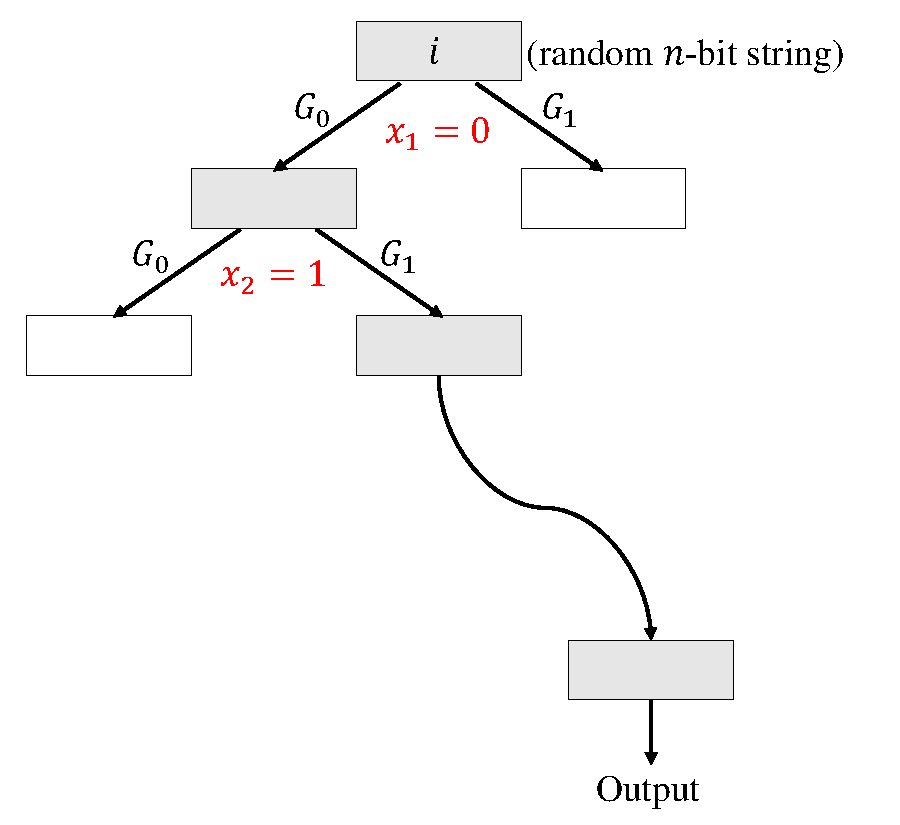
\includegraphics[width=\textwidth]{Old Scribe Notes/binary-tree.pdf}
    \caption{View the construction as a binary tree}
    \label{fig:binary-tree}
\end{marginfigure}

\begin{theorem}\label{theorem:ggm}
    The function ensemble $\{F_n\}_{n \in \mathbb{N}}$ constructed above is pseudorandom.
\end{theorem}

\proof
Assume for the sake of contradiction that $\{F_n\}_{n \in \mathbb{N}}$ is not a PRF.
Then there exists a non-uniform PPT oracle adversary $\ma$ that can distinguish $\{F_n\}_{n \in \mathbb{N}}$ from $\{R_n\}_{n \in \mathbb{N}}$. Below, via a hybrid argument, we prove that this contradicts the fact that $G$ is a PRG; we will construct an adversary $\mathcal{B}$ that can distinguish between a sample from $U_{2n}$ and $G(U_{n})$. We will prove for a fixed $n$, and the proof can be easily extended to all $n \in \mathbb{N}$.\smallskip

\noindent \textbf{Hybrids}. Consider the sequence of hybrids $H_i$ for $i \in \{ 0, 1, \cdots, n\}$ where the hybrid $i$ is defined as follows:
\[H_{i}^{(K_i)} (x_1x_2\ldots x_n ):= G_{x_n}(G_{x_{n-1}} (\cdots(G_{x_{i+1}}(K_i(x_1\dots x_{i-1}x_i))) \cdots  )), \]
where $K_i$ is a random function from $\{0,1\}^{i}$ to $\{0,1\}^n$. Intuitively, hybrid $H_i$ corresponds to a binary tree of depth $n$ where the nodes of levels $0$ to $i$ correspond to random values and the nodes at levels $i+1$ to $n$ correspond to pseudorandom values. By inspection, observe that hybrids $H_0$ and $H_n$ are identical to a pseudorandom function and a random function, respectively. Note that we cannot yet reduce the computational indistinguishability of $H_i$ and $H_{i+1}$ to security of the PRG $G$ because the adversary can make multiple oracle queries at different inputs.\smallskip

\noindent \textbf{Sub-hybrids}. We show that $H_{i}$ and $H_{i+1}$ are indistinguishable by considering a sequence of sub-hybrids $H_{i,j}$ for $j \in \{0,\ldots q\}$, where $q$ is the number of oracle queries made by $\mathcal{A}$\footnote{Observe that $\mathcal{A}$ can make at most polynomial in $n$ oracle queries. Looking ahead, our outer adversary $\mathcal{B}$ can either take $q$ as the max queries allowed to $\mathcal{A}$, or guess the number, and double the guess each time if it's an under-estimate.}.
Intuitively, with each sub-hybrid $H_{i,j}$, at level $i+1$ in the tree, we will fix the first $j$ oracle queries made by $\mathcal{A}$ to be output of random functions and the rest to be output of PRG. Let $R_i: \{0, 1\}^i \to \{0, 1\}^n$ and $S_{i}: \{0, 1\}^{i+1} \to \{0, 1\}^n$ be two random functions.
We define sub-hybrid $H_{i,j}^{(R_i, S_{i})}(x_1x_2\dots x_n)$ algorithmically as follows:
\begin{enumerate}
    \item Initialize a list $L \gets \{\}$ to store the $i$-bit prefixes of the queries made by $\mathcal{A}$.
    \item If $|L| < j$ or $(x_1\dots x_i) \in L$\footnote{Captures the first $j$ queries or any query with repeated $i$-bit prefix to a previous query.}:
          \begin{enumerate}[noitemsep,nolistsep]
              \item Set $y \gets S_i(x_1\dots x_i x_{i+1})$.
              \item Append $(x_1\dots x_i)$ to $L$.
              \item For $a \in i+2 \dots n$: update $y \gets G_{x_a}(y)$.
          \end{enumerate}
    \item Else:
          \begin{enumerate}[noitemsep,nolistsep]
              \item Set $y \gets R_i(x_1\dots x_i)$.
              \item For $a \in i+1 \dots n$: update $y \gets G_{x_a}(y)$.
          \end{enumerate}
    \item Output $y$.
\end{enumerate}

Note that $H_{i, 0}$ is the same as $H_i$ and $H_{i, q}$ is the same as $H_{i+1}$. Since we assumed that $\mathcal{A}$ can distinguish between $H_0$ and $H_n$, by triangle inequality, there exists a $i^*, j^*$ such that it can distinguish $H_{i^*,j^*}$ and $H_{i^*,j^*+1}$. We now focus on these two sub-hybrids\footnote{Looking ahead, the outer adversary $\mathcal{B}$ can guess $i^*, j^*$; total choices are bounded by polynomial in $n$. To simplify the proof, we will assume that $\mathcal{B}$ already knows this $i^*, j^*$.}. Consider the $j^*+1$-th query made by $\mathcal{A}$ (i.e. the first query where $|L|=j$). Observe that this query cannot have the same $i$-bit prefix as any of the previous queries. Because if it did, then the output distribution of the two hybrids would be identical, and that contradicts our assumption about $\mathcal{A}$'s distinguishing power. Therefore, the $j^*+1$-th query has to be a new query, and this query is the only place where the two hybrids differ.\smallskip

\noindent \textbf{Outer adversary $\mathcal{B}$}. Now we are ready to construct our outer adversary $\mathcal{B}$ that can distinguish between $U_{2n}$ and $G(U_n)$. $\mathcal{B}^{\mathcal{A}, i^*, j^*}(1^n, z)$, where $z \in \{0, 1\}^{2n}$ ($z$ could be either from $U_{2n}$ or $G(U_n)$) and we assume the knowledge of $i^*, j^*$\footnote{As mentioned before, it can be guessed with slight loss in distinguishing advantage.}, operates as follows:
\begin{enumerate}
    \item Parse $z$ as $z_0||z_1$, where $z_0, z_1 \in \{0, 1\}^n$.
    \item For all the oracle queries from $\mathcal{A}$ except the $j^*+1$-th query, respond as $H_{i^*,j^*}$\footnote{The outer adversary $\mathcal{B}$ runs a random function in polynomial time in $n$ via lazy sampling. It generates a random output on a new input and caches responses to previous inputs.}.
    \item For the $j^*+1$-th query $(x_1\dots x_n)$, do the following:
          \begin{enumerate}
              \item Set $y \gets z_{x_{i^*+1}}$.
              \item For $a \in i^*+2 \dots n$: update $y \gets G_{x_a}(y)$.
              \item Respond with $y$.
          \end{enumerate}
    \item Output whatever $\mathcal{A}$ outputs.
\end{enumerate}

We assumed that $\mathcal{A}$ can distinguish between $H_{i^*, j^*}$ and $H_{i^*, j^*+1}$, so by contrapositive of the Sunglass Lemma, $\mathcal{B}$ can distinguish between $U_{2n}$ and $G(U_n)$. This contradicts that $G$ is a PRG.

%where $q_{i+1}$ is the number of the distinct $i-bit$ prefixes of the queries of $\mathcal{A}$.\footnote{Observe that $q_{i+1}$ for each appropriate choice of $i$ is bounded by the running time of $\mathcal{A}$. Hence, this value is bounded by a polynomial in the security parameter.}
%We define hybrid $H_{i,j}$ for $j =0$ to be same as hybrid $H_{i}$. Additionally, for $j >0$ hybrid $H_{i,j}$ is defined to be exactly the same as hybrid $H_{i,j-1}$ except the response provided to the attacker for the $j^{th}$ distinct $i-bit$ prefix query of $\mathcal{A}$. Let this prefix be $x^*_n x^*_{n-1} \ldots x^*_{i}$. Note that in hybrid $H_{i,j-1}$ the children of the node $x^*_n x^*_{n-1} \ldots x^*_{i}$ correspond to two pseudorandom values. In hybrid $H_{i,j}$ we replace these two children with random values. By careful inspection, it follows that hybrid $H_{i,q_{i+1}}$ is actually $H_{i+1}$. All we are left to prove is that hybrid $H_{i,j}$ and $H_{i,j+1}$ are indistinguishable for the appropriate choices of $j$ and we prove this below.
%Now we are ready to construct an adversary $\mathcal{B}$ that  distinguishes $U_{2n}$ from $G(U_n)$: On input $T \in\{0, 1\}^{2n}$ ($T$ could be either from $U_{2n}$ or $G(U_n)$),
%construct a full binary tree of depth $n$ that is exactly the same as $H_{i,j}$ except replacing the children of  $x^*_n x^*_{n-1} \ldots x^*_{i}$ by the value $T$.
%Observe that the only difference between $H_{i,j}$ and $H_{i,j+1}$ is that values corresponding to nodes $x_n^*\ldots x_i^* 0$ and $x_n^*\ldots x_i^* 1$ are pseudorandom or random respectively. $\mathcal{B}$ uses the value $T$ to generate these two nodes. Hence success in  distinguishing hybrids $H_{i,j}$ and $H_{i,j+1}$ provides a successful attack for $\mathcal{B}$ in violating security of the pseudorandom generator.
\qed







\section{PRFs from DDH: Naor-Reingold PRF}
We will now describe a PRF function family $F_n: \mathcal{K} \times \{0,1\}^n \rightarrow \mathbb{G}_n$ where DDH is assumed to be hard for  $\{\mathbb{G}_n\}$ and $\mathcal{K}$ is the key space.
The key for the PRF $F_n$ will be $K =  (h, u_1, \ldots u_n)$, where $u,u_0\ldots u_n$ are sampled uniformly from $|\mathbb{G}_n|$, $g$ is the generator of $\mathbb{G}_n$ and $h = g^u$. Compared to the previous construction (Theorem~\ref{theorem:ggm}), there are two differences to note already: the key is polynomially longer and the output space is $\mathbb{G}_n$ instead of $\{0, 1\}^n$.

\[F_n(K,x) = h^{\prod_{i} u_i^{x_i}}\]

Next, we will prove that the function $F_n$ is a pseudo-random function or that $\{F_n\}$ is a pseudo-random function ensemble.\footnote{Here, we require that adversary distinguish the function $F_n$ from a random function from $\{0,1\}^n$ to $\mathbb{G}_n$. Note that the output range of the function is $\mathbb{G}_n$. Moreover, note that the distribution of random group elements in $\mathbb{G}_n$ might actually be far from uniformly random strings.}
\begin{lemma}
    Assuming the DDH Assumption (see Definition~\ref{def:ddh}) for $\{\mathbb{G}_n\}$ is hard, we have that $\{F_n\}$ is a pseudorandom function ensemble.
\end{lemma}
\begin{proof}
    The proof of this lemma is similar to the proof of Theorem~\ref{theorem:ggm} except for some subtle differences that arise from number theory\footnote{At a high-level, we can no longer fix nodes in the same level of the tree arbitrarily. Fixing one node has implications for how other nodes will be changed. This is because we have a fixed basis in the key.}.

    Let $R_n$ be random function from $\{0,1\}^n \rightarrow \mathbb{G}_n$. Then we want to prove that for all non-uniform PPT adversaries $\mathcal{A}$ we have that:
    \[\mu(n) = \left|\Pr[\mathcal{A}^{F_n}(1^n) =1] -  \Pr[\mathcal{A}^{R_n}(1^n) =1]\right|\]
    is a negligible function. \smallskip

    \noindent \textbf{Hybrids}. For the sake of contradiction, we assume that the function $F_n$ is not pseudorandom. Next, towards a contradiction, we consider a sequence of hybrid functions $H^0_n \ldots H^n_n$.
    For $j \in \{0, \dots, n\}$, let $S^j_n: \{0, 1\}^j \to \{0, 1, \dots, |\mathbb{G}_n|-1\}$, then hybrid $H_n^j$ is defined as\footnote{Algorithmically, $H_n^j((u,u_{j+1}\ldots u_n),x)$ is computed as:
    \begin{enumerate}
        \item Set $y \gets S_n^j(x_1\ldots x_j)$.
        \item For $i = j+1 \dots n$: update $y \gets y \cdot u_i^{x_i}$.
        \item Output $g^y$.
    \end{enumerate}

    }:
    \begin{equation*}
        H_n^j((u,u_{j+1}\ldots u_n),x) = \big(g^{S_n^j(x_1\ldots x_j)}\big)^{\prod_{i=j+1}^n u_i^{x_i}}
    \end{equation*}
    where $S_n^0(\cdot)$ is the constant function with output $u$. Observe that $H_n^0$ is the same as the function $F_n$ and $H_n^n$ is the same as the function $R_n$\footnote{A uniform group element is equivalently sampled by first sampling an exponent in the order of the group.}. Thus, by a hybrid argument and triangle inequality, we conclude that there exists $j^* \in \{0,\ldots n-1\}$, such that
    \[\left|\Pr[\mathcal{A}^{H_n^{j^*}}(1^n) =1] -  \Pr[\mathcal{A}^{H_n^{j^*+1}}(1^n) =1]\right|\]
    is a non-negligible function. Now all we are left to show is that this implies an attacker that refutes the DDH assumption.\smallskip

    \noindent \textbf{Sub-hybrids}. The proof of this claim follows by a sequence of $q+1$ sub-hybrids $H_n^{j, 0}, \dots, H_n^{j, q}$, where $q$ is the (polynomially bounded by $n$) running time of $\mathcal{A}$. For the simplicity of exposition, we abuse the notation and denote $q(n)$ by $q$. Let $C_n^j: \{0, 1\}^j \to \{0, \dots, |\mathbb{G}_n|-1\}$ and $D_n^j: \{0, 1\}^{j+1} \to \{0, \dots, |\mathbb{G}_n|-1\}$ be two random functions, and $C_n^0(\cdot) = u$. We define sub-hybrid $H_n^{j, k}\big((u, u_{j+1}\ldots u_n),(x_1\dots x_n)\big)$ for $k \in \{0, \dots, q\}$ as follows:
    \begin{enumerate}
        \item Initialize a list $L \gets \{\}$ to store the $j$-bit prefixes of the queries made by $\mathcal{A}$.
        \item If $|L|<k$ or $(x_1\cdots x_j) \in L$:
              \begin{enumerate}[noitemsep,nolistsep]
                  \item Set $y \gets D^j_n(x_1\dots x_{j+1})$.
                  \item Append $(x_1\dots x_j)$ to $L$.
                  \item For $i = j+2 \dots n$: update $y \gets y \cdot u_i^{x_i}$.
              \end{enumerate}
        \item Else
              \begin{enumerate}[noitemsep,nolistsep]
                  \item Set $y \gets C^j_n(x_1\dots x_j)$.
                  \item For $i = j+1 \dots n$: update $y \gets y \cdot u_i^{x_i}$.
              \end{enumerate}
        \item Output $g^y$.
    \end{enumerate}

    It is easy to see that $H_n^{j, 0}$ is the same as $H_n^j$ and $H_n^{j, q}$ is the same as $H_n^{j+1}$.
    Again, we use hybrid argument to conclude that there exists $j^*, k^*$ such that $\mathcal{A}$ can distinguish between $H_n^{j^*, k^*}$ and $H_n^{j^*, k^*+1}$ with non-negligible probability. We now focus on these two sub-hybrids. Consider the $k^*+1$-th oracle query made by $\mathcal{A}$. Following an identical argument we used in the proof of Theorem~\ref{theorem:ggm}, this query cannot be a repeat of a query made before, and this query is the only place where the two sub-hybrids differ.\smallskip

    \noindent \textbf{Outer adversary $\mathcal{B}$}. The construction of the outer adversary $\mathcal{B}$ is a bit different from the proof of Theorem~\ref{theorem:ggm}. Intuitively, unlike Theorem~\ref{theorem:ggm}, outer adversary cannot simply replace the $k^*+1$-th query with the DDH challenge in isolation from the rest of the queries made by $\mathcal{A}$. This is because the pseudorandom nodes in the tree are tied together by the DDH relation, and are not independent, i.e., all pseudorandom sibling nodes on the same level of the tree are set apart by a common exponent.

    $\mathcal{B}$ gets as challenge either a DDH tuple $(g, A=g^a, B=g^b, C=g^{ab})$ or a uniform tuple $(g, A=g^a, B=g^b, C=g^c)$ where $a, b, c$ are uniform in $\{0, \dots, |\mathbb{G}|-1\}$. We construct $\mathcal{B}^{\mathcal{A}, j^*, k^*}\big(1^n, (g, A, B, C)\big)$ as follows:
    \begin{enumerate}
        \item Sample $u, u_{j^*+1}, \ldots u_n$ uniformly from $\{0, \dots, |\mathbb{G}_n|-1\}$.
        \item For first $k^*$ queries from $\mathcal{A}$, respond as $H_n^{j^*, k^*}((u, u_{j^*+1}, \ldots u_n),\cdot)$.
        \item For the $k^*+1$-th query $(x_1\ldots x_n)$, do the following:
              \begin{enumerate}[noitemsep,nolistsep]
                  \item Set $y \gets A$ if $x_{j^*+1} = 0$ and $y \gets C$ if $x_{j^*+1} = 1$.
                  \item For $i = j^*+2 \dots n$: update $y \gets y \cdot u_i^{x_i}$.
                  \item Output $g^y$.
              \end{enumerate}
        \item For the rest of the queries $(x_1\ldots x_n)$, do the following:
              \begin{enumerate}[noitemsep,nolistsep]
                  \item Set $y \gets C^j_n(x_1\ldots x_j)$.
                  \item For $i = j^*+2 \dots n$: update $y \gets y \cdot u_i^{x_i}$.
                  \item If $x_{j^*+1} = 0$, output $g^y$, else output\footnote{Recall that $B=g^b$, so $B^y = g^{y\cdot b} = g^{y\cdot b^x_{j^*+1}}$. Therefore, the DDH relation is properly set for all pseudorandom nodes.} $B^y$.
              \end{enumerate}
        \item Output whatever $\mathcal{A}$ outputs.
    \end{enumerate}

    By the construction of $\mathcal{B}$, if $(g, A, B, C)$ is a DDH tuple, then the distribution of oracle responses seen by $\mathcal{A}$ are exactly the same as the responses seen in the hybrid $H_n^{j^*, k^*}$. Otherwise, they are the same as hybrid $H_n^{j^*, k^*+1}$.
    We assumed that $\mathcal{A}$ can distinguish between $H_n^{j^*, k^*}$ and $H_n^{j^*, k^*+1}$, therefore $\mathcal{B}$ can distinguish between a DDH tuple and a uniform tuple. This contradicts our assumption that DDH is hard.

    %Without loss of generality we assume that $\mathcal{A}$ never makes the same query twice.
    %More specifically, we consider a sequence of functions $F_n^{k,t}$ where $t \in \{0,T\}$, $F_n^{k,0}$ is same as $F_n^{k}$ and $F_n^{k,T}$ is same as $F_n^{k+1}$. In particular, we explain how $F_n^{k,t}$ answers queries by $\mathcal{A}$.\footnote{As assumed earlier, keep in mind that $\mathcal{A}$ never makes the same query twice.} Let $x^1, \ldots x^t$ be the first $t$ queries made by $\mathcal{A}$. For any query, $x$ made by $\mathcal{A}$ such that the first $k$ bits of $x$ match the first $k$ bits of one of $x_1, \ldots x_y$ answer as $F_n^{k+1}$ else answer as $F_n^{k}$. Now we can conclude that there exists a $t$ such that $F_n^{k,t}$ and $F_n^{k,t+1}$ are distinguishable with non-negligible probability.
    %Finally, we will show that using an adversary that can distinguish between $F_n^{k,t}$ and $F_n^{k,t+1}$ we need to construct an adversary $\mathcal{B}$ that refutes the DDH assumption. We leave construction of this adversary as an exercise.
\end{proof}


\newpage
\section*{Exercises}
\begin{exercise}
    % \newcommand{\bit}{\{0,1\}}

    Prove or disprove: If $f$ is a one-way function, then the following function $B:\bit^*\to\bit$ is a hardconcentrate predicate for $f$. The function $B(x)$ outputs the inner product modulo 2 of the first $\lfloor |x|/2\rfloor$ bits of $x$ and the last $\lfloor |x|/2\rfloor$ bits of $x$.
\end{exercise}

\begin{exercise}
    Let $\phi(n)$ denote the first $n$ digits of $\pi = 3.141592653589\ldots$ after the decimal in binary ($\pi$ in its binary notation looks like $11.00100100001111110110101010001000100001\ldots$).

    Prove the following: if one-way functions exist, then there exists a one-way function $f$ such that the function $B:\{0,1\}^* \rightarrow \{0,1\}$ is not a hard concentrate bit of $f$. The function $B(x)$ outputs $\langle x, \phi(|x|)\rangle$, where
    \[\langle a, b\rangle := \sum_{i=1}^n a_i b_i \mod 2\]
    for the bit-representation of $a = {a_1a_2\cdots a_n}$ and $b= {b_1b_2\cdots b_n}$.
\end{exercise}

\begin{exercise}
    If $f: \{0,1\}^{n}\times \{0,1\}^n\rightarrow \{0,1\}^n$  is PRF, then in which of the following cases is $g: \{0,1\}^{n}\times \{0,1\}^n\rightarrow \{0,1\}^n$ also a PRF? \begin{enumerate} \item $g(K,x) = f(K,f(K,x))$ \item $g(K,x) = f(x,f(K,x))$ \item $g(K,x) = f(K,f(x,K))$
    \end{enumerate}
\end{exercise}

\begin{exercise}[Puncturable PRFs.] Puncturable PRFs are PRFs for which a key can be given out such that, it allows evaluation of the PRF on all inputs, except for one designated input.

    %\newcommand{\negl}{\mathsf{negl}}
    \newcommand{\A}{\mathcal{A}}
    \newcommand{\F}{F}
    \newcommand{\KeyF}{\mathsf{Key}_{\F}}
    \newcommand{\PunctureF}{\mathsf{Puncture}_{\F}}
    \newcommand{\EvalF}{\mathsf{Eval}_{\F}}


    A puncturable pseudo-random function $\F$ is given by a triple of efficient algorithms ($\KeyF$,$\PunctureF$, and $\EvalF$), satisfying the following conditions:
    \begin{itemize}
        \item[-] \textbf{Functionality preserved under puncturing}: For every $x^*, x \in \{0,1\}^{n}$ such that $x^* \neq x$, we have that:
              $$\Pr[\EvalF(K,x) = \EvalF(K_{x^*},x) : K \gets \KeyF(1^n), K_{x^*} = \PunctureF(K,x^*)] = 1$$
        \item[-] \textbf{Pseudorandom at the punctured point}: For every $x^*\in \{0,1\}^n$ we have that for every polysize adversary $\A$ we have that:
              $$|\Pr[\A(K_{x^*}, \EvalF(K,x^*)) = 1] - \Pr[\A(K_{x^*}, \EvalF(K,U_n)) = 1]|= \negl(n)$$
              where $K \gets \KeyF(1^n)$ and $K_S = \PunctureF(K,x^*)$. $U_n$ denotes the uniform distribution over $n$ bits.
    \end{itemize}

    Prove that: If one-way functions exist, then there exists a puncturable PRF family that maps $n$ bits to $n$ bits. \\
    \textbf{Hint:} The GGM tree-based construction of PRFs from a length doubling pseudorandom generator (discussed in class) can be adapted to construct a puncturable PRF. Also note that $K$ and $K_{x^*}$ need not be the same length.
\end{exercise}
%
%\subsection{Application}
%Consider an interesting game: Alice and Bob are talking on the phone.
%Alice flips a coin, and Bob guesses whether it's head or tail.
%But the problem is how can Alice convince Bob that the coin is indeed head or tail?
%If we have pseudorandom functions, the problem could be easily solved.
%
%Assume we have a PRF $F_n: \{0, 1\}^n \rightarrow \{0, 1\}^n$.
%Alice and Bob have a shared key $i \in \{0, 1\}^n$, then $f_i(\cdot)$ is shared information.
%Now Alice has a message $m \in \{0, 1\}^n$ and wants to let Bob guess it,
%the procedure consists of three steps.
%\begin{enumerate}[(a)]
%    \item Alice chooses a string $r \in \{0, 1\}^n$, and sends to Bob  $m' = f_i(r) \oplus m$ ;
%    \item Bob guesses $m$;
%    \item Alice sends $r$ to Bob.
%\end{enumerate}
%In step (a), since $F_n$ is PRF, all the information that Bob gets is a random $n$-bit string, so it will not influence his behavior in step (b).
%Then in step (c), Bob receives $r$ and will be convinced that the true value of $m$ is $f_i(r) \oplus m'$.
%

\chapter{Private-Key Cryptography}
%\newcommand{\key}{\mathsf{k}}
% \newcommand{\gen}{\mathsf{Gen}}
\section{Private-Key Encryption}
The first primitive that we will study in private-key cryptography is that of private-key encryption.
When talking about private-key encryption, we will be working in a setting where two players, Alice and Bob, are attempting to communicate with each other.

Alice and Bob want to communicate with each other.
For simplicity, let's assume that only Alice wants to send a message to Bob.
The crucial property that they want is that no eavesdropper attempting to listen to the conversation should be able to decipher the contents of the message being sent.
\begin{comment}
\begin{center}
    \begin{tikzpicture}
        \draw;
    \end{tikzpicture}
\end{center}    
\end{comment}
% Figure A goes here

To achieve this, the two employ the following communication protocol:
\begin{enumerate}
    \item A priori, Alice and Bob generate a key $k$ and distribute it in such a way that only the two of them know what $k$ is.
    \item Using $k$, Alice can encrypt her message $m$, to turn it into a ciphertext $c$, which she sends over to Bob. 
    \item Upon receiving $c$, Bob can decrypt its contents and recover $m$ by using $k$.
\end{enumerate}
This meta-scheme implies a couple of requirements.
First of all, we want Bob to indeed be able to recover $m$ when decrypting $c$ with $k$.
It is no use having a communication scheme where the message received is not the one sent. We will call this requirement \textit{correctness}.
The second requirement, which we have already mentioned, is \textit{confidentiality}.
To reiterate, \textit{confidentiality} means that no eavesdropper that manages to get a hold of $c$ should be able to learn anything about $c$ that they do not already know (assuming they have no knowledge of the key $k$).
In addition to these two fundamental requirements, we might also impose that our private-key encryption scheme guarantees \textit{integrity} and \textit{authenticity}.
By \textit{integrity}, we mean that Bob should be able to detect that the message $c$ has been tampered with prior to him receiving it.
By \textit{authenticity}, we mean that Bob should be able to verify that the message he received was indeed sent by Alice, and not some adversary interfering with the conversation.

Now that we have some intuitive understanding of what we are trying to achieve, let us attempt to ground it in mathematics.

\begin{definition}[Private-Key Encryption Scheme]
    A private-key encryption scheme $\Pi$ is a tuple $\Pi = (\gen, \enc, \dec)$, where $\gen, \enc$, and $\dec$ are algorithms such that:
    \begin{enumerate}
        \item $\gen(1^n) \rightarrow k$
        \item $\enc(k, m) \rightarrow c$
        \item $\dec(k, c) \rightarrow m'$
    \end{enumerate}

    where $n$ is a security parameter and $k, c, m, m' \in \{0, 1\}^*$
\end{definition}


%Alice might also want to be able to deal with attackers that can tamper with $c$.
%When Bob receives something, he wants to be able to verify that it indeed comes from Alice.

\begin{comment}
$$\Pi = (Gen, Enc, Dec)$$
$$Gen(1^n) \rightarrow k$$
$$Enc(k, m) \rightarrow c$$
$$Dec(k, c) \rightarrow m'$$
\end{comment}


% Besides correctness, we want our cryptosystem to be \textit{confidential}.

Now, we will formalize the requirements of our cryptosystem.
Our first requirement is correctness, which is defined below:

\begin{definition}[(Perfect) Correctness]
    We say that a private-key encryption scheme $\Pi = (\gen, \enc, \dec)$ is \emph{(perfectly) correct} if 
    $\forall n, k \in \gen(1^n), m \in \{0,1\}^{*}$,
    $$\Pr[\dec(k,\enc(k,m)) = m] = 1$$
\end{definition}
That is, if $c = \enc(k, m)$, then Bob is guaranteed to recover $m$ by running $\dec(k, c)$. Note that for a fixed-length encryption scheme, we require that $m \in \bit^{l(n)}$.

Next, we will formalize what we mean by \textit{confidentiality}.
We will often use the terms \textit{confidentiality} and \textit{security} interchangeably in the context of private-key encryption schemes.
Our first definition of confidentiality is called IND Security, stated below:

\begin{definition}[IND Security]
    $\forall m_0, \forall m_1$ s.t. $|m_0| = |m_1|= l(n)$ and $\forall$ nu-PPT $\ma$ we have
    $$|\Pr[\ma(1^n, \enc(k, m_0)) = 1 \; | \; k \leftarrow \gen(1^n)] - |\Pr[\ma(1^n, \enc(k, m_1)) = 1 \; | \; k \leftarrow \gen(1^n)]| = neg(n)$$ 
\end{definition}
Note that this is not a particularly good definition of security, in the sense that the attacker is very limited in what they are allowed to do.
Specifically, all that $\ma$ can do is take a look at the encryption of $m_0$ and $m_1$ and must decide which one is the plaintext.
We need a more usable and realistic definition of security.
For this reason, we will allow the attacker to have oracle access to the encryption function, $\enc(k, \cdot)$.
In other words, $\ma$ will be able to craft their own ciphertexts, which it can then use to break the security of the encryption scheme.
We shall dub this new definition of security \textit{Chosen Plaintext Attack Security}, or \textit{CPA Security} for short.

%Informally, this means that the ciphertext $c$ should hide everything about $m$ that Eve doesn't already know.

In defining \textit{CPA Security}, we will also introduce a new method for defining private-key encryption schemes: the game-style definition.
The rationale behind this change in style is that probabilistic definitions, while precise and rigorous, are rather cumbersome to work with, especially in the context of secure communication.
Therefore, we will adopt this new paradigm, which will make it easier to work with and reason about private-key encryption schemes.

\marginnote[-1.5in]{
\procedureblock[linenumbering]{$ \pcnotionstyle{Priv\pcmathhyphen{}}\indcpa_{\Pi}^{\adv}(\secpar)$}{
 b \getsr \bin \\
  \key  \getsr \gen ( \secparam ) \\
 ( \state ,m_0 ,m_1) \getsr \adv^{\enc ( \key ,\cdot )} ( \secparam) \\
 c \getsr \enc ( \key ,m_b ) \\
 b' \getsr \adv^{\enc ( \key ,\cdot )} ( \state , c ) \\
 \pcreturn b = b' \land |m_0| = |m_1| = l(n)
 }}

\begin{definition}[CPA Security]
    A private-key encryption scheme $\Pi = (\gen,\enc,\dec)$ is CPA-secure if $\forall$ nu-PPT $\ma$
    $$\advantage{\indcpa}{\Pi,\adv} = \Big| \Pr[\pcnotionstyle{Priv\pcmathhyphen{}}\indcpa_\Pi^\adv(\secpar) =1] -\frac{1}{2}\Big|$$
    is a negligible function.
\end{definition}
Observe that in this new game-style definition, we have a concrete notion of the order in which each action is taken.
One important detail to note (and that is more evident in a game-style definition) is that in our \textit{CPA Security} definition,
the key $k$ is sampled \textit{before} $m_0$ and $m_1$ are fixed.
This is in contrast to \textit{IND Security}, in which the messages $m_0$ and $m_1$ are chosen before the key $k$ is sampled\footnote{This is an important detail because if $m_0$ and $m_1$ are chosen before $k$ is sampled, then giving oracle access to $\ma$ is not much help.}.

To further illustrate this point, consider the following scheme, which is secure in IND but insecure in CPA:
\begin{itemize}
    \item $\gen(\secparam):$
    \begin{enumerate}
        \item $k \leftarrow \gen(\secparam)$
        \item $x \getsr \{0, 1\}^n$
        \item $k' = (k, x)$
    \end{enumerate}
    \item $\enc'(k', m)L:$
    \begin{enumerate}
        \item if $m = x$, then output $x$
        \item else, output $\enc(k,m)||x$
    \end{enumerate}
\end{itemize}

%We formalize this property in our definition of \emph{Chosen Plaintext Attack Security}, or \textit{CPA Security} for short.
%In presenting this new definition, we will also introduce the notion of game-style definitions.
%The motivation behind this is that probabilistic definitions, such as the ones we have been working with thus far, are cumbersome and difficult to work with.
%Game-style definitions are easier to work with and give us better ideas of 

%Properties we want:
%\begin{itemize}
%    \item $c$ should hide everything about $m$ that Eve doesn't already know
%\end{itemize}

%There are many ways to formally define this notion
%Formally,

% To make this definition of security more robust, we allow $\ma$ to have oracle access\footnote{In other words, $\ma$ can create their own ciphertexts.} to $\enc(k, \cdot)$
% This definition is not good enough because we are fixing $m_0$ and $m_1$. * ASK ABOUT THIS.

\begin{comment}
\begin{definition}[$\pcnotionstyle{Priv\pcmathhyphen{}}\indcpa$] A private-key encryption scheme $\Pi = (\gen,\enc,\dec)$ is $\pcnotionstyle{Priv\pcmathhyphen{}}\indcpa$-secure if 
$$ \advantage{\indcpa}{\Pi,\adv} = \Large\mid \Pr[\pcnotionstyle{Priv\pcmathhyphen{}}\indcpa_\Pi^\adv(\secpar) =1] -\frac12\Large\mid$$
is a negligible function. 
\end{definition}    
The main difference is when the key $k$ is sampled.
In the first definition, $m_0$ and $m_1$ are fixed before $k$ is sampled,
whereas in the second definition, $k$ is sampled before $m_0$ and $m_1$ are fixed.
\end{comment}

% Transition from the probability-style definitions to game-style definitions.


The final security notion we will define is CCA (chosen-ciphertext attack) security.
Here, the attacker is allowed oracle access to both the encryption and the decryption functions.
Let $L$ be the working list of queries that $\ma$ has made to $Dec(k, \cdot)$.
Then $\pcnotionstyle{Priv\pcmathhyphen{}}\indcca_{\Pi}^{\adv}(\secpar)$ is defined as:
\marginnote[-1.5in]{
\procedureblock[linenumbering]{$ \pcnotionstyle{Priv\pcmathhyphen{}}\indcca_{\Pi}^{\adv}(\secpar)$}{
 b \getsr \bin \\
  \key  \getsr \gen ( \secparam ) \\
 ( \state ,m_0 ,m_1) \getsr \adv^{\enc ( \key ,\cdot ), \dec(k, \cdot)} ( \secparam) \\
 c \getsr \enc ( \key ,m_b ) \\
 b' \getsr \adv^{\enc ( \key ,\cdot ), \dec(k, \cdot)} ( \state , c ) \\
 \pcreturn b = b' \land |m_0| = |m_1| \land c \notin L
 }}

\begin{definition}[CCA Security]
    A private-key encryption scheme $\Pi = (\gen,\enc,\dec)$ is CCA-secure if $\forall$ nu-PPT $\ma$
    $$\advantage{\indcca}{\Pi,\adv} = \Big| \Pr[\pcnotionstyle{Pri\pcmathhyphen{}}\indcca_\Pi^\adv(\secpar) =1] -\frac{1}{2}\Big|$$
    is a negligible function.
\end{definition}

$\Pi$ is a fixed-length encryption scheme for length $l(n)$ if $l(n)$ is polynomial in $n$ and $|m_0| = |m_1| = l(n)$.

\begin{theorem}
    If F is a PRF then the scheme $\Pi = (\gen, \enc, \dec)$ given below is a secure encryption scheme for length $n$.

    \begin{itemize}
        \item $\gen(\secparam)$:
        \begin{enumerate}
            \item output $k \getsr \{0, 1\}^n$
        \end{enumerate}
        \item $\enc(k, m)$:
        \begin{enumerate}
            \item $r \getsr \{0, 1\}^n$
            \item output $(r, F_k(r) \oplus m)$
        \end{enumerate}
        \item $\dec(k, c=(c_1, c_2))$:
        \begin{enumerate}
            \item output $c_2 \oplus F_k(c_1)$
        \end{enumerate}
    \end{itemize}

\end{theorem}

\proof
Assume there exists a nu-PPT $\ma$ that is able to break CPA security of $\Pi$.
Then we can construct a nu-PPT adversary $\mb$ that breaks the PRF $F$.
The strategy is outlined in the figure below:

\begin{center}
    \begin{tikzpicture}
        % Adversary B rectangle
        \draw (0,8) node[anchor=north west]{$\mb$};
        \draw (0, 0) rectangle (12, 8);
        \draw[thick, ->] (0,7)--(-1,7) node[anchor=south west] {$x$};
        \draw[thick, ->] (-1,6)--(0,6) node[anchor=south east] {$F(x)$};
        \draw (9, 0.5) rectangle (11, 7.5);
        % Adversary A rectangle
        \draw (9,7.5) node[anchor=north west]{$\ma$};
        \draw[thick, ->] (0,2)--(-1,2) node[anchor=south west] {$x^*$};
        \draw[thick, ->] (-1,1)--(0,1) node[anchor=south east] {$F(x^*)$};
        \draw[thick, ->] (0,0)--(-1,0) node[anchor=north west] {Output $b = b'$};
        \draw[thick, ->] (9,7)--(8,7) node[anchor=south west] {$m$};
        \draw[thick, ->] (8,6)--(9,6) node[anchor=south east] {$c$};
        \draw[thick, ->] (9,5)--(8,5) node[anchor=south west] {$m_0, m_1$};
        % \draw[thick, ->] (8,4)--(9,4) node[anchor=south east] {$c^*$};
        % \draw[thick, ->] (9,3)--(8,3) node[anchor=south west] {$m$};
        \draw[thick, ->] (8,2)--(9,2) node[anchor=south east] {$c^*$};
        \draw[thick, ->] (9,1)--(8,1) node[anchor=south west] {$b$};
        % Pseudocode
        \draw (3, 7) node[anchor=west] {1. $x \getsr \{0, 1\}^n$};
        \draw (3, 6) node[anchor=west] {2. $y = F(x)$};
        \draw (3, 5) node[anchor=west] {3. $c = (x, m \oplus y)$};
        \draw (3, 3) node[anchor=west] {4. $b \getsr \{0, 1\}$};
        \draw (3, 2) node[anchor=west] {5. $x^* \getsr \{0, 1\}^n$};
        \draw (3, 1) node[anchor=west] {6. $c^* = (x^*, m_b \oplus F(x^*))$};
        % Other arrows
        \draw[thick, dashed, red, ->] (2.75, 7)--(0.25,7);

        \draw[thick, dashed, red, ->] (0.25,6)--(2.75, 6);

        \draw[thick, dashed, blue, ->] (6.25, 5) .. controls (6.75, 5) and (7.4, 6) .. (7.75,6);

        \draw[thick, dashed, red, <-] (0.25, 2)--(2.75,2);

        \draw[thick, dashed, red, ->] (0.25, 1)--(2.75,1);

        \draw[thick, dashed, blue, ->] (5.25, 1.35) .. controls (6.75, 1.75) .. (7.75,2);

        \draw[thick, dashed, blue, <-] (0,0.1) .. controls (7, 0.2) .. (7.75, 1);

    \end{tikzpicture}
\end{center}
After running this procedure, we guess ``Pseudorandom" if $b=b'$.
Else, we guess random.


Now we argue that 
$$|\Pr[B^{F_n(\cdot)}(1^n) = 1] - \Pr[\mb^{F_n(\cdot)}(1^n) = 1]|$$
is non-negligible.

\begin{align*}
    |\Pr[B^{F_n(\cdot)}(1^n) = 1] - \Pr[\mb^{F_n(\cdot)}(1^n) = 1]| &\ge \frac{1}{2} + \epsilon(n) - (\frac{1}{2} + \frac{q(n)}{2^n}) \\
    &= \epsilon(n) - \frac{q(n)}{2^n}
\end{align*}
\qed

\begin{theorem}
    No deterministic encryption scheme $\Pi$ can be CPA Secure.
\end{theorem}

\proof
The proof of this claim is simple.
If we have a deterministic encryption scheme, then when we get $c^*$, we can again try to encrypt a message and check if $c = c^*$
\qed


\subsection{Counter Mode Encryption}
One construction of a CCA-secure cipher is by the use of the counter mode.

\begin{itemize}
    \item $\enc(k, (m_1,...,m_\ell)):$
    \begin{algorithmic}[1]
        \item $r \getsr \{0,1\}^n$
        \item Output $c = (r, m_1 \oplus F_k(r+1),
            m_2 \oplus F_k(r+2),
            ...,
            m_\ell \oplus F_k(r+\ell))$
    \end{algorithmic}
\end{itemize}

Consider the following picture:

\begin{center}
    \begin{tikzpicture}
        \draw[thick, ->] (0,0)--(12,0);
        \draw[thick, -] (1, 0.25)--(1, -0.25);
        \draw (1, -0.75) node[anchor=south] {$x_1$};
        \draw[thick, -] (2.5, 0.25)--(2.5, -0.25);
        \draw (2.5, -0.75) node[anchor=south] {$x_1 + q(n)$};
        \draw[thick, -] (5, 0.25)--(5, -0.25);
        \draw (5, -0.75) node[anchor=south] {$x_2$};
        \draw[thick, -] (6.5, 0.25)--(6.5, -0.25);
        \draw (6.5, -0.75) node[anchor=south] {$x_2 + q(n)$};
        \draw (9.5, -0.75) node[anchor=south] {...};
    \end{tikzpicture}
\end{center}

Then the probability of breaking this cipher is
$$\frac{2q(n) - 1}{2^n} \cdot q(n)$$

In practice, we use block ciphers, which are stronger primitives.

\section{Message Authentication Codes}
Now we address the question of how we can guarantee the \textit{integrity} of a message.
To achieve this, we will construct a new primitive, called a \textit{message authentication code}, or MAC for short. MACs generate a verifiable tag $t$ for a message $m$ that cannot be forged.

When sending a message, Alice sends the pair $(m, t)$.
Once Bob receives the message, he runs $\Verify(k, m, t)$.
He accepts the message if $\Verify(k, m, t) = 1$, otherwise he rejects the message.
The formal definition is stated below:
\begin{definition}[Private-Key Encryption Scheme]
    A MAC scheme $\Pi$ is a tuple of algorithms $\Pi = (\gen, \mac, \Verify)$, with the following syntax:
    \begin{enumerate}
        \item $k \leftarrow \gen(1^n)$
        \item $t \leftarrow \mac(k,m)$
        \item $0/1 \leftarrow \Verify(k, m, t)$
    \end{enumerate}
    where $n$ is a security parameter and $k, m \in \{0, 1\}^{l(n)}$
\end{definition}

We impose the following \textit{correctness} requirement on our MACs:
\begin{definition}[MAC Correctness]
    $$\forall n, k \in \gen(1^n), m \in \{0, 1\}^*, \Pr[\Verify(k, m, \mac(k, m)) = 1] = 1$$
\end{definition}

We also want the message authentication codes to be \textit{unforgeable}.
That is, given a message $m$, a nu-PPT attacker $\ma$ should only be able to forge a tag $t$ for $m$ with negligible probability.
\begin{definition}[EUF-CMA Security]
    A MAC scheme $\Pi = (\gen,\mac,\Verify)$ is EUF-CMA-secure if $\forall$ nu-PPT $\ma$,
    $$\Big| \Pr\left[\mathsf{MAC}\pcmathhyphen{}\mathsf{forge}_{\cA, \Pi}(\secpar) =1\right]\Big| = \negl$$
\end{definition}

\begin{definition}[$\mathsf{MAC}\pcmathhyphen{}\mathsf{forge}_{\cA, \Pi}(\secpar)$]
$ $
   \begin{enumerate}
        \item \textbf{Setup:} The challenger samples $k$ uniformly from the key space. $\cA$ is given $1^n$.
        \item \textbf{Query:} The adversary submits a message $m^{(i)}$; then the challenger computes a tag $t^{(i)} \gets \mac(k, m^{(i)})$ and sends it to the adversary. The adversary may submit any polynomial number of message queries.

        Let $\mathcal{Q} = \{(m^{(1)}, t^{(1)}), \dots, (m^{(q)}, t^{(q)})\}$ be the set of messages $m^{(i)}$ submitted in the query phase along with the tags $t^{(i)}$ computed by $\mac$.
        \item \textbf{Forgery:} The adversary outputs a message-tag pair $(m^*, t^*)$. The output of the game is $1$ if $(m^*,t^*) \notin \mathcal{Q}$ and $\Verify(k, m^*, t^*) = 1$. The output is $0$ otherwise.
    \end{enumerate}
\end{definition}


%\marginnote[-1.5in]{
%\procedureblock[linenumbering]{$ \pcnotionstyle{OLDPri\pcmathhyphen{}}\indcpa_{\Pi}^{\adv}(\secpar)$}{
% b \sample \bin \\
%  \key  \sample \gen ( \secparam ) \\
% ( \state ,m_0 ,m_1) \sample \adv^{\enc ( \key ,\cdot )} ( \secparam) \\
% c \sample \enc ( \key ,m_b ) \\
% b' \sample \adv^{\enc ( \key ,\cdot )} ( \state , c ) \\
% \pcreturn b = b' }
% }

 
\DIFaddbegin \newcommand{\nonnegl}{\mathsf{nonnegl}}


\section{\DIFadd{Fixed-length MACs}}

\DIFadd{Previously, we defined what a MAC is, and specified correctness and security definitions for MACs. In this section, we'll define a fixed-length MAC for length \mbox{%DIFAUXCMD
$\ell(n)$
}%DIFAUXCMD
.
}

\begin{theorem}
    \DIFadd{If \mbox{%DIFAUXCMD
$F : \{0, 1\}^n \to \{0, 1\}^n$
}%DIFAUXCMD
is a secure PRF, then the MAC scheme \mbox{%DIFAUXCMD
$\Pi = (\mathsf{Gen}, \mathsf{Mac}, \mathsf{Verify})$
}%DIFAUXCMD
constructed below has EUF-CMA security.
}

    \begin{itemize}
        \item \DIFadd{\mbox{%DIFAUXCMD
$\gen(1^n):$
}%DIFAUXCMD
}\begin{algorithmic}
            \item \DIFadd{Output \mbox{%DIFAUXCMD
$k \getsr \{0, 1\}^n$
}%DIFAUXCMD
}\end{algorithmic}
        \item \DIFadd{\mbox{%DIFAUXCMD
$\mac(k,m):$
}%DIFAUXCMD
}\begin{algorithmic}
            \item \DIFadd{Output \mbox{%DIFAUXCMD
$t = F_k(m)$
}%DIFAUXCMD
}\end{algorithmic}
        \item \DIFadd{\mbox{%DIFAUXCMD
$\Verify(k, m, t)$
}%DIFAUXCMD
}\begin{algorithmic}
            \item \DIFadd{If \mbox{%DIFAUXCMD
$t = F_k(m)$
}%DIFAUXCMD
, then return \mbox{%DIFAUXCMD
$1$
}%DIFAUXCMD
. 
            }\item \DIFadd{Otherwise return \mbox{%DIFAUXCMD
$0$
}%DIFAUXCMD
.
        }\end{algorithmic}
    \end{itemize}
    \DIFadd{That is, we just compute the PRF on our message as the MAC.
}\end{theorem}

\begin{proof}
    \DIFadd{To prove security, suppose for contradiction that there exists an adversary \mbox{%DIFAUXCMD
$A$
}%DIFAUXCMD
that breaks the security for \mbox{%DIFAUXCMD
$\Pi$
}%DIFAUXCMD
. We'd like to construct an adversary \mbox{%DIFAUXCMD
$B$
}%DIFAUXCMD
that breaks the security of the PRF.
}

    \DIFadd{Here, the adversary \mbox{%DIFAUXCMD
$A$
}%DIFAUXCMD
expects queries for tags, given messages as input. \mbox{%DIFAUXCMD
$B$
}%DIFAUXCMD
can simply forward these requests on to \mbox{%DIFAUXCMD
$F$
}%DIFAUXCMD
, and return the response back to \mbox{%DIFAUXCMD
$A$
}%DIFAUXCMD
. Further, \mbox{%DIFAUXCMD
$A$
}%DIFAUXCMD
outputs a pair \mbox{%DIFAUXCMD
$(m^*, t^*)$
}%DIFAUXCMD
, which \mbox{%DIFAUXCMD
$B$
}%DIFAUXCMD
can send \mbox{%DIFAUXCMD
$m^*$
}%DIFAUXCMD
to \mbox{%DIFAUXCMD
$F$
}%DIFAUXCMD
, and output whether \mbox{%DIFAUXCMD
$t = t^*$
}%DIFAUXCMD
.
}

    \begin{center}
        \begin{tikzpicture}
            \draw (3, 0) rectangle (8, 5.5);
            \draw (5, 0.5) rectangle (7.5, 5);
            \node at (3.25, 5.25) {\mbox{%DIFAUXCMD
$B$
}%DIFAUXCMD
};
            \node at (5.25, 4.75) {\mbox{%DIFAUXCMD
$A$
}%DIFAUXCMD
};

            \draw (5.5, 4) edge[->] node[right, pos=0] {\mbox{%DIFAUXCMD
$m$
}%DIFAUXCMD
} (2.5, 4)
                (2.5, 3.5) edge[->] node[right, pos=1] {\mbox{%DIFAUXCMD
$t$
}%DIFAUXCMD
} (5.5, 3.5);
            \node[left] at (2.5, 3.75) {\mbox{%DIFAUXCMD
$F_k$
}%DIFAUXCMD
};
            \node at (5.5, 3.1) {\mbox{%DIFAUXCMD
$\vdots$
}%DIFAUXCMD
};
            \node at (4.5, 3.1) {\mbox{%DIFAUXCMD
$\vdots$
}%DIFAUXCMD
};
            \draw (5.5, 2.5) edge[->] node[right, pos=0] {\mbox{%DIFAUXCMD
$(m^*, t^*)$
}%DIFAUXCMD
} (4.5, 2.5);

            \draw (3.5, 2.5) edge[->] node[right, pos=0] {\mbox{%DIFAUXCMD
$m^*$
}%DIFAUXCMD
} (2.5, 2.5);
            \node[left] at (2.5, 2.25) {\mbox{%DIFAUXCMD
$F_k$
}%DIFAUXCMD
};
            \draw (2.5, 2) edge[->] node[right, pos=1] {\mbox{%DIFAUXCMD
$t$
}%DIFAUXCMD
} (3.5, 2);
            \draw (3.5, 1) edge[->] node[right, pos=0] {\mbox{%DIFAUXCMD
$t \overset{?}{=} t^*$
}%DIFAUXCMD
} (2.5, 1);
        \end{tikzpicture}
    \end{center}

    \DIFadd{Analyzing the probability for \mbox{%DIFAUXCMD
$B$
}%DIFAUXCMD
, we have
    }\[
        \DIFadd{\abs{\Pr(B^{F_k(\cdot)}(1^n) = 1) - \Pr(B^{R_n(\cdot)}(1^n) = 1)}
        = \abs{\varepsilon_A(n) - \frac{1}{2^n}}
        = \nonnegl(n)
    .}\]
    \DIFadd{Here, the first term is because the correctness follows immediately from the correctness of \mbox{%DIFAUXCMD
$A$
}%DIFAUXCMD
, and the second term is due to the fact that the output of \mbox{%DIFAUXCMD
$R_n$
}%DIFAUXCMD
is random.
}\end{proof}

\section{\DIFadd{Variable-length MACs}}

\DIFadd{Now, let us look at messages with lengths that are a multiple of \mbox{%DIFAUXCMD
$n$
}%DIFAUXCMD
. In particular, we have a few blocks \mbox{%DIFAUXCMD
$m_1, \ldots, m_{\ell}$
}%DIFAUXCMD
, each of size \mbox{%DIFAUXCMD
$n$
}%DIFAUXCMD
. There are a few ways to do this, but we'll look at a method similar to the counter mode we looked at last time.
}

\begin{center}
    \begin{tikzpicture}
        \node (m1) at (0, 2) {\mbox{%DIFAUXCMD
$m_1$
}%DIFAUXCMD
};
        \node (m2) at (1, 2) {\mbox{%DIFAUXCMD
$m_2$
}%DIFAUXCMD
};
        \node (m3) at (2, 2) {\mbox{%DIFAUXCMD
$m_3$
}%DIFAUXCMD
};
        \node (mdots) at (3, 2) {\mbox{%DIFAUXCMD
$\cdots$
}%DIFAUXCMD
};
        \node (ml) at (4, 2) {\mbox{%DIFAUXCMD
$m_{\ell}$
}%DIFAUXCMD
};

        \node[draw] (fk1) at (0, 0) {\mbox{%DIFAUXCMD
$F_k$
}%DIFAUXCMD
};
        \node[draw] (fk2) at (1, 0) {\mbox{%DIFAUXCMD
$F_k$
}%DIFAUXCMD
};
        \node[draw] (fk3) at (2, 0) {\mbox{%DIFAUXCMD
$F_k$
}%DIFAUXCMD
};
        \node at (3, 0) {\mbox{%DIFAUXCMD
$\ldots$
}%DIFAUXCMD
};
        \node[draw] (fkl) at (4, 0) {\mbox{%DIFAUXCMD
$F_k$
}%DIFAUXCMD
};

        \node[outer sep=0pt, inner sep=0pt, draw, circle] (fk1+m2) at (1, 1) {\mbox{%DIFAUXCMD
$+$
}%DIFAUXCMD
};
        \node[outer sep=0pt, inner sep=0pt, draw, circle] (fk2+m3) at (2, 1) {\mbox{%DIFAUXCMD
$+$
}%DIFAUXCMD
};
        \node[outer sep=0pt, inner sep=1pt] (xor-dots) at (3, 1) {\mbox{%DIFAUXCMD
$\ldots$
}%DIFAUXCMD
};
        \node[outer sep=0pt, inner sep=0pt, draw, circle] (dots+ml) at (4, 1) {\mbox{%DIFAUXCMD
$+$
}%DIFAUXCMD
};

        \draw (m1) edge[->] (fk1)
            (m2) edge[->] (fk1+m2)
            (m3) edge[->] (fk2+m3)
            (ml) edge[->] (dots+ml);

        \draw[->] (fk1) -- ++(0.5, 0) |- (fk1+m2);
        \draw[->] (fk2) -- ++(0.5, 0) |- (fk2+m3);
        \draw[->] (fk3) -- ++(0.5, 0) |- (xor-dots);

        \draw[->] (xor-dots) -- (dots+ml);
        \draw (fk1+m2) edge[->] (fk2)
            (fk2+m3) edge[->] (fk3)
            (dots+ml) edge[->] (fkl);
        \draw (fkl) edge[->] ++(1, 0);
    \end{tikzpicture}
\end{center}

\DIFadd{This construction avoids having to store a tag equal in length to the message, but this is not secure, due to length extension attacks. In particular, suppose we query for the tag \mbox{%DIFAUXCMD
$t$
}%DIFAUXCMD
associated with \mbox{%DIFAUXCMD
$0^n$
}%DIFAUXCMD
. We can then query another tag \mbox{%DIFAUXCMD
$t'$
}%DIFAUXCMD
for \mbox{%DIFAUXCMD
$0^n \oplus t$
}%DIFAUXCMD
. Observe here that \mbox{%DIFAUXCMD
$t'$
}%DIFAUXCMD
is also the tag for \mbox{%DIFAUXCMD
$0^{2n}$
}%DIFAUXCMD
.
}

\DIFadd{A solution is to use different keys for each PRF, but this isn't too efficient, since we're still calling the PRF once per block of length \mbox{%DIFAUXCMD
$n$
}%DIFAUXCMD
. We'll instead improve this to use only one block cipher call---we do some preprocessing and only call \mbox{%DIFAUXCMD
$F_k$
}%DIFAUXCMD
once on the output of the preprocessing.
}

\DIFadd{In particular, we'll claim that applying a universal hash function to the input and then applying the block cipher is a secure MAC.
}

\begin{definition}[Universal Hash Function]
    \DIFadd{A function \mbox{%DIFAUXCMD
$h : \mathcal{F} \times \mathcal{F}^* \to \mathcal{F}$
}%DIFAUXCMD
(where \mbox{%DIFAUXCMD
$\mathcal{F}$
}%DIFAUXCMD
is a field of size \mbox{%DIFAUXCMD
$2^m$
}%DIFAUXCMD
) is a universal hash function if for all \mbox{%DIFAUXCMD
$m, m' \in \mathcal{F}^{\le \ell}$
}%DIFAUXCMD
(i.e. \mbox{%DIFAUXCMD
$m$
}%DIFAUXCMD
and \mbox{%DIFAUXCMD
$m'$
}%DIFAUXCMD
have length at most \mbox{%DIFAUXCMD
$\ell$
}%DIFAUXCMD
),
    }\[
        \DIFadd{\Pr_s(h(s, m) = h(s, m')) \le \frac{\ell}{\abs{F}}
    .}\]
    \DIFadd{That is, the probability of collision is small.
}\end{definition}

\DIFadd{Crucially here, we fix \mbox{%DIFAUXCMD
$m$
}%DIFAUXCMD
and \mbox{%DIFAUXCMD
$m'$
}%DIFAUXCMD
, and we sample \mbox{%DIFAUXCMD
$s$
}%DIFAUXCMD
. (If we fix an \mbox{%DIFAUXCMD
$s$
}%DIFAUXCMD
, we can almost surely find an \mbox{%DIFAUXCMD
$m$
}%DIFAUXCMD
and \mbox{%DIFAUXCMD
$m'$
}%DIFAUXCMD
that collide.)
}

\DIFadd{Today, we'll look at the following function:
}\[
    \DIFadd{h(s, m_0, \ldots, m_{\ell - 1}) = m_0 + m_1 s + m_2 s^2 + \cdots + m_{\ell - 1} s^{\ell - 1} + s^{\ell}
.}\]

\begin{claim}
    \DIFadd{The function defined by
    }\[
        \DIFadd{h(s, m_0, \ldots, m_{\ell - 1}) = m_0 + m_1 s + m_2 s^2 + \cdots + m_{\ell - 1} s^{\ell - 1} + s^{\ell}
    }\]
    \DIFadd{is a universal hash function.
}\end{claim}

\begin{proof}
    \DIFadd{We'd like to argue that for a fixed \mbox{%DIFAUXCMD
$m$
}%DIFAUXCMD
and \mbox{%DIFAUXCMD
$m'$
}%DIFAUXCMD
, and a random \mbox{%DIFAUXCMD
$s$
}%DIFAUXCMD
, the probability that there is a collision is at most \mbox{%DIFAUXCMD
$\frac{\ell}{\abs{\mathcal{F}}}$
}%DIFAUXCMD
.
}

    \DIFadd{We'll look at
    }\[
        \DIFadd{h(x, m_0, \ldots, m_t) - h(x, m_0', \ldots, m_t') = (m_0 - m_0') + \cdots + (m_{t - 1} - m_{t-1}') x^{\ell - 1}
    .}\]
    \DIFadd{If there is a collision, this difference is 0. The probability that this polynomial of degree at most \mbox{%DIFAUXCMD
$\ell$
}%DIFAUXCMD
has a zero at \mbox{%DIFAUXCMD
$x$
}%DIFAUXCMD
is at most \mbox{%DIFAUXCMD
$\frac{\ell}{\abs{\mathcal{F}}}$
}%DIFAUXCMD
, since it has at most \mbox{%DIFAUXCMD
$\ell$
}%DIFAUXCMD
zeroes. This means that \mbox{%DIFAUXCMD
$h$
}%DIFAUXCMD
is indeed a universal hash function.
}\end{proof}

\begin{claim}
    \DIFadd{The MAC given by \mbox{%DIFAUXCMD
$F_k(h(s, m_1, \ldots, m_{\ell}))$
}%DIFAUXCMD
, for the universal hash function \mbox{%DIFAUXCMD
$h$
}%DIFAUXCMD
given prior, is secure. (This is a slight variation on the Carter--Wegman MAC.)
}\end{claim}

\begin{proof}
    \DIFadd{Suppose for contradiction that there exists a nu-PPT \mbox{%DIFAUXCMD
$A$
}%DIFAUXCMD
that breaks the security of this scheme.
}

    \DIFadd{Here, for appropriately generated \mbox{%DIFAUXCMD
$k$
}%DIFAUXCMD
and \mbox{%DIFAUXCMD
$s$
}%DIFAUXCMD
, \mbox{%DIFAUXCMD
$A$
}%DIFAUXCMD
makes queries \mbox{%DIFAUXCMD
$m \mapsto F_k(h_s(m))$
}%DIFAUXCMD
, and outputs \mbox{%DIFAUXCMD
$(m^*, t^*)$
}%DIFAUXCMD
.
}

    \DIFadd{We'd like to create an adversary \mbox{%DIFAUXCMD
$B$
}%DIFAUXCMD
that either breaks the security of the PRF, or breaks the security of the universal hash function.
}

    \DIFadd{\mbox{%DIFAUXCMD
$B$
}%DIFAUXCMD
will start by sampling \mbox{%DIFAUXCMD
$s \in \mathcal{F}$
}%DIFAUXCMD
. When given the query for \mbox{%DIFAUXCMD
$m_1$
}%DIFAUXCMD
, it computes \mbox{%DIFAUXCMD
$h_s(m_1)$
}%DIFAUXCMD
and queries for \mbox{%DIFAUXCMD
$F_k(h_s(m_1))$
}%DIFAUXCMD
, which it sends back to \mbox{%DIFAUXCMD
$A$
}%DIFAUXCMD
. If \mbox{%DIFAUXCMD
$F_k$
}%DIFAUXCMD
was actually pseudorandom, then \mbox{%DIFAUXCMD
$A$
}%DIFAUXCMD
is given a pseudorandom input, and if \mbox{%DIFAUXCMD
$F_k$
}%DIFAUXCMD
was random \mbox{%DIFAUXCMD
$R_n$
}%DIFAUXCMD
, then \mbox{%DIFAUXCMD
$A$
}%DIFAUXCMD
is given a random input.
}

    \DIFadd{\mbox{%DIFAUXCMD
$A$
}%DIFAUXCMD
must still be able to generate pairs \mbox{%DIFAUXCMD
$(m^*, t^*)$
}%DIFAUXCMD
even when given a random input, due to the security of the PRF.
}

    \begin{center}
        \begin{tikzpicture}
            \draw (2, 0) rectangle (8, 5.5);
            \draw (5, 0.5) rectangle (7.5, 5);
            \node at (2.25, 5.25) {\mbox{%DIFAUXCMD
$B$
}%DIFAUXCMD
};
            \node at (5.25, 4.75) {\mbox{%DIFAUXCMD
$A$
}%DIFAUXCMD
};

            \node at (3.5, 4.5) {sample \mbox{%DIFAUXCMD
$s \in \mathcal{F}$
}%DIFAUXCMD
};

            \node (hsm) at (3.5, 4) {\mbox{%DIFAUXCMD
$h_s(m)$
}%DIFAUXCMD
};
            \draw (5.5, 4) edge[->] node[right, pos=0] {\mbox{%DIFAUXCMD
$m$
}%DIFAUXCMD
} (hsm)
                (hsm) edge[->] (1.5, 4)
                (1.5, 3.5) edge[->] node[right, pos=1] {\mbox{%DIFAUXCMD
$t$
}%DIFAUXCMD
} (5.5, 3.5);
            \node[left] at (1.5, 3.75) {\mbox{%DIFAUXCMD
$F_k$
}%DIFAUXCMD
};
            \node at (5.5, 3.1) {\mbox{%DIFAUXCMD
$\vdots$
}%DIFAUXCMD
};
            \node at (4.5, 3.1) {\mbox{%DIFAUXCMD
$\vdots$
}%DIFAUXCMD
};

            \node (hash-m-star) at (3.5, 2.5) {\mbox{%DIFAUXCMD
$h_s(m^*)$
}%DIFAUXCMD
};
            \draw (5.5, 2.5) edge[->] node[right, pos=0] {\mbox{%DIFAUXCMD
$(m^*, t^*)$
}%DIFAUXCMD
} (hash-m-star)
                (hash-m-star) edge[->] (1.5, 2.5);
            \node[left] at (1.5, 2.25) {\mbox{%DIFAUXCMD
$F_k$
}%DIFAUXCMD
};
            \draw (1.5, 2) edge[->] node[right, pos=1] {\mbox{%DIFAUXCMD
$t$
}%DIFAUXCMD
} (3.5, 2);
            \draw (3.5, 1) edge[->] node[right, pos=0] {\mbox{%DIFAUXCMD
$t \overset{?}{=} t^*$
}%DIFAUXCMD
} (1.5, 1);
        \end{tikzpicture}
    \end{center}

    \DIFadd{Let \mbox{%DIFAUXCMD
$E$
}%DIFAUXCMD
be the event that there exists an \mbox{%DIFAUXCMD
$m, m' \in L \cup \{m^*\}$
}%DIFAUXCMD
, such that \mbox{%DIFAUXCMD
$h_s(m) = h(m')$
}%DIFAUXCMD
. If \mbox{%DIFAUXCMD
$E$
}%DIFAUXCMD
does not happen, then the hash function never collides. This means that the attacker only sees random values depending on distinct inputs, so this reduces to the case from earlier (when the MAC is just \mbox{%DIFAUXCMD
$F_k$
}%DIFAUXCMD
).
}

    \DIFadd{As such, we'd like to show that collisions in \mbox{%DIFAUXCMD
$h_s(\cdot)$
}%DIFAUXCMD
occur with negligible probability.
}

    \DIFadd{To show this, suppose for contradiction that collisions actually do occur with non-negligible probability. We then want to construct an adversary \mbox{%DIFAUXCMD
$B$
}%DIFAUXCMD
utilizing \mbox{%DIFAUXCMD
$A$
}%DIFAUXCMD
that just outputs \mbox{%DIFAUXCMD
$m$
}%DIFAUXCMD
and \mbox{%DIFAUXCMD
$m'$
}%DIFAUXCMD
such that when \mbox{%DIFAUXCMD
$s$
}%DIFAUXCMD
is sampled, \mbox{%DIFAUXCMD
$h_s(m) = h_s(m')$
}%DIFAUXCMD
with high probability.
}

    \DIFadd{\mbox{%DIFAUXCMD
$B$
}%DIFAUXCMD
will pick a random \mbox{%DIFAUXCMD
$i, j \in \{1, \ldots, q+1\}$
}%DIFAUXCMD
(here suppose \mbox{%DIFAUXCMD
$i < j$
}%DIFAUXCMD
), where \mbox{%DIFAUXCMD
$q$
}%DIFAUXCMD
is the number of MAC queries. We then run \mbox{%DIFAUXCMD
$A$
}%DIFAUXCMD
until the \mbox{%DIFAUXCMD
$j$
}%DIFAUXCMD
th query. Taking the \mbox{%DIFAUXCMD
$i$
}%DIFAUXCMD
th and \mbox{%DIFAUXCMD
$j$
}%DIFAUXCMD
th query, we then output \mbox{%DIFAUXCMD
$m_i$
}%DIFAUXCMD
and \mbox{%DIFAUXCMD
$m_j$
}%DIFAUXCMD
as our pair of messages. We still need to entertain the queries made by \mbox{%DIFAUXCMD
$A$
}%DIFAUXCMD
, so we can just return random values for tags (giving the same value if it requests it for the same message).
}

    \begin{center}
        \begin{tikzpicture}
            \draw (2, 0) rectangle (8, 6);
            \draw (5, 0.5) rectangle (7.5, 5.5);
            \node at (2.25, 5.75) {\mbox{%DIFAUXCMD
$B$
}%DIFAUXCMD
};
            \node at (5.25, 5.25) {\mbox{%DIFAUXCMD
$A$
}%DIFAUXCMD
};

            \node[align=center] at (3.5, 5) {\small \mbox{%DIFAUXCMD
$i, j \xleftarrow{\$} \{1, \ldots, q+1\}$
}%DIFAUXCMD
};

            \draw (5.5, 4) edge[->] node[right, pos=0] {\mbox{%DIFAUXCMD
$m_1$
}%DIFAUXCMD
} (4.5, 4)
                (4.5, 3.5) edge[->] node[left, pos=0] {sample \mbox{%DIFAUXCMD
$t_1$
}%DIFAUXCMD
} node[right, pos=1] {\mbox{%DIFAUXCMD
$t_1$
}%DIFAUXCMD
} (5.5, 3.5);
            \node at (5.5, 3.1) {\mbox{%DIFAUXCMD
$\vdots$
}%DIFAUXCMD
};
            \node at (4.5, 3.1) {\mbox{%DIFAUXCMD
$\vdots$
}%DIFAUXCMD
};

            \draw (5.5, 2.5) edge[->] node[right, pos=0] {\mbox{%DIFAUXCMD
$m_i$
}%DIFAUXCMD
} (4.5, 2.5)
                (4.5, 2) edge[->] node[left, pos=0] {sample \mbox{%DIFAUXCMD
$t_i$
}%DIFAUXCMD
} node[right, pos=1] {\mbox{%DIFAUXCMD
$t_i$
}%DIFAUXCMD
} (5.5, 2);
            \node at (5.5, 1.6) {\mbox{%DIFAUXCMD
$\vdots$
}%DIFAUXCMD
};
            \node at (4.5, 1.6) {\mbox{%DIFAUXCMD
$\vdots$
}%DIFAUXCMD
};

            \draw (5.5, 1) edge[->] node[right, pos=0] {\mbox{%DIFAUXCMD
$m_j$
}%DIFAUXCMD
} (4.5, 1);

            \draw (3, 0.5) edge[->] node[right, pos=0] {\mbox{%DIFAUXCMD
$(m_i, m_j)$
}%DIFAUXCMD
} (1.5, 0.5);
        \end{tikzpicture}
    \end{center}

    \DIFadd{By assumption, we know that \mbox{%DIFAUXCMD
$E$
}%DIFAUXCMD
occurs with non-negligible probability. That is, among the queries made by \mbox{%DIFAUXCMD
$A$
}%DIFAUXCMD
, there is a non-negligible probability that \mbox{%DIFAUXCMD
$h_s(m_i) = h_s(m_j)$
}%DIFAUXCMD
. Since here the implementation of \mbox{%DIFAUXCMD
$B$
}%DIFAUXCMD
just picks out a pair of random queries from those made by \mbox{%DIFAUXCMD
$A$
}%DIFAUXCMD
, the pair \mbox{%DIFAUXCMD
$(m_i, m_j)$
}%DIFAUXCMD
output by \mbox{%DIFAUXCMD
$B$
}%DIFAUXCMD
also has a collision with non-negligible probability. (In particular, with probability \mbox{%DIFAUXCMD
$\Pr(E) / q^2$
}%DIFAUXCMD
.
}

    \DIFadd{This breaks the definition of a universal hash function, which is a contradiction.
}\end{proof}

\DIFadd{So far, we know how to generate tags of fixed length, and of lengths that are a multiple of \mbox{%DIFAUXCMD
$n$
}%DIFAUXCMD
. If we have a message that is not a multiple of \mbox{%DIFAUXCMD
$n$
}%DIFAUXCMD
, we could potentially just pad the input with 0's, but this causes an issue, as \mbox{%DIFAUXCMD
$m$
}%DIFAUXCMD
and \mbox{%DIFAUXCMD
$m \concat 0$
}%DIFAUXCMD
have the same tag.
}

\DIFadd{Instead, one solution is to put the size of the message in the first block, and we can still put the padding at the end. This way, if the messages differ by length, the first block will be different, and if the messages do not differ by length, then we're essentially just ignoring the padding. This gives us a MAC for arbitrary-length messages.
}

\section{\DIFadd{Authenticated Encryption Schemes}}

\DIFadd{We've talked about confidentiality and integrity separately, but generally we want both properties---when Alice sends a message to Bob, we'd like for any eavesdropper to be unable to recover the message, }\emph{\DIFadd{and}} \DIFadd{we'd like Bob to be able to verify that the message actually came from Alice.
}

\DIFadd{A scheme that achieves both of these conditions is called an }\emph{\DIFadd{authenticated encryption scheme}}\DIFadd{.
}

\begin{definition}[Authenticated Encryption Scheme]
    \DIFadd{A scheme \mbox{%DIFAUXCMD
$\Pi$
}%DIFAUXCMD
is an }\emph{\DIFadd{authenticated encryption scheme}} \DIFadd{if it is CPA-secure, and it has ciphertext integrity (CI).
}\end{definition}

\begin{definition}[Ciphertext Integrity (CI)]
    \DIFadd{Consider the following game for the scheme \mbox{%DIFAUXCMD
$\Pi = (\mathsf{Gen}, \mathsf{Enc}, \mathsf{Dec})$
}%DIFAUXCMD
.
}

    \begin{algorithmic}[1]
        \Function{CI\mbox{%DIFAUXCMD
${}_{\Pi}^A$
}%DIFAUXCMD
}{\mbox{%DIFAUXCMD
$n$
}%DIFAUXCMD
}
            \State \DIFadd{\mbox{%DIFAUXCMD
$k \gets \mathsf{Gen}(1^n)$
}%DIFAUXCMD
}\State \DIFadd{\mbox{%DIFAUXCMD
$c^* \gets A^{\mathsf{Enc}(k, \cdot)}(1^n)$
}%DIFAUXCMD
}\State \DIFadd{\mbox{%DIFAUXCMD
$L \gets$
}%DIFAUXCMD
the list of queries made by \mbox{%DIFAUXCMD
$A$
}%DIFAUXCMD
}\State \Return \DIFadd{\mbox{%DIFAUXCMD
$(\mathsf{Dec}(k, c^*) \ne \bot) \land (c^* \notin L)$
}%DIFAUXCMD
}\EndFunction
    \end{algorithmic}

    \DIFadd{A scheme has ciphertext integrity if for all nu-PPT \mbox{%DIFAUXCMD
$A$
}%DIFAUXCMD
, \mbox{%DIFAUXCMD
$\Pr(\mathrm{CI}_{\Pi}^A)$
}%DIFAUXCMD
is negligible.
}\end{definition}

\DIFadd{Observe that an authenticated encryption scheme is also CCA-secure, since the CI property says that the adversary can never generate a valid ciphertext. This means that whenever an adversary requests the decryption of a ciphertext, we can always return \mbox{%DIFAUXCMD
$\bot$
}%DIFAUXCMD
(unless they previously requested a ciphertext for a message, and wants to decode that ciphertext). This means that the decryption oracle is essentially useless, and this reduces to the CPA case.
}

\DIFadd{Next, we'll construct an authenticated encryption scheme, called ``Encrypt-then-MAC'', utilizing a CPA-secure encryption scheme and an EUF-CMA MAC scheme.
}

\begin{claim}
    \DIFadd{Let \mbox{%DIFAUXCMD
$\Pi_e = (\mathsf{Gen}_e, \mathsf{Enc}_e, \mathsf{Dec}_e)$
}%DIFAUXCMD
be a CPA-secure encryption scheme, and let \mbox{%DIFAUXCMD
$\Pi_m = (\mathsf{Gen}_m, \mathsf{Mac}_m, \mathsf{Verify}_m)$
}%DIFAUXCMD
be an EUF-CMA-secure MAC scheme.
}

    \DIFadd{The following scheme \mbox{%DIFAUXCMD
$\Pi = (\mathsf{Gen}, \mathsf{Enc}, \mathsf{Dec})$
}%DIFAUXCMD
is an authenticated encryption scheme.
}

    \begin{algorithmic}[1]
        \Function{Gen}{\mbox{%DIFAUXCMD
$1^n$
}%DIFAUXCMD
}
            \State \DIFadd{\mbox{%DIFAUXCMD
$k_e \gets \mathsf{Gen}_e(1^n)$
}%DIFAUXCMD
}\State \DIFadd{\mbox{%DIFAUXCMD
$k_m \gets \mathsf{Gen}_m(1^n)$
}%DIFAUXCMD
}\State \Return \DIFadd{\mbox{%DIFAUXCMD
$(k_e, k_m)$
}%DIFAUXCMD
}\EndFunction
        \Statex
        \Function{Enc}{\mbox{%DIFAUXCMD
$(k_e, k_m), m$
}%DIFAUXCMD
}
            \State \DIFadd{\mbox{%DIFAUXCMD
$c \gets \mathsf{Enc}_e(k_e, m)$
}%DIFAUXCMD
}\State \DIFadd{\mbox{%DIFAUXCMD
$t \gets \mathsf{Mac}_m(k_m, c)$
}%DIFAUXCMD
}\State \Return \DIFadd{\mbox{%DIFAUXCMD
$(c, t)$
}%DIFAUXCMD
}\EndFunction
        \Statex
        \Function{Dec}{\mbox{%DIFAUXCMD
$(k_e, k_m), (c, t), m$
}%DIFAUXCMD
}
            \If {\DIFadd{\mbox{%DIFAUXCMD
$\mathsf{Verify}_m(k_m, c, t)$
}%DIFAUXCMD
}}
                \State \Return \DIFadd{\mbox{%DIFAUXCMD
$\mathsf{Dec}_e(k_e, c)$
}%DIFAUXCMD
}\Else
                \State \Return \DIFadd{\mbox{%DIFAUXCMD
$\bot$
}%DIFAUXCMD
}\EndIf 
        \EndFunction
    \end{algorithmic}
\end{claim}

\begin{proof}
    \DIFadd{Suppose for contradiction that we have an adversary \mbox{%DIFAUXCMD
$A$
}%DIFAUXCMD
that breaks the CPA security of \mbox{%DIFAUXCMD
$\Pi$
}%DIFAUXCMD
. The CPA game allows for queries of the ciphertext for messages \mbox{%DIFAUXCMD
$m$
}%DIFAUXCMD
, produces a pair \mbox{%DIFAUXCMD
$m_0, m_1$
}%DIFAUXCMD
, and then gets \mbox{%DIFAUXCMD
$c^* = \mathsf{Enc}(k, m_B)$
}%DIFAUXCMD
, and \mbox{%DIFAUXCMD
$A$
}%DIFAUXCMD
eventually outputs \mbox{%DIFAUXCMD
$b'$
}%DIFAUXCMD
to identify which message was encrypted.
}

    \DIFadd{We'd like to construct another adversary \mbox{%DIFAUXCMD
$B$
}%DIFAUXCMD
, which breaks the CPA-security of \mbox{%DIFAUXCMD
$\Pi_e$
}%DIFAUXCMD
. The only difference here is the MACs, so \mbox{%DIFAUXCMD
$B$
}%DIFAUXCMD
can sample a \mbox{%DIFAUXCMD
$k_m \gets \mathsf{Gen}_m(1^n)$
}%DIFAUXCMD
, and perform all of the MACs itself.
}

    \DIFadd{In particular, when \mbox{%DIFAUXCMD
$A$
}%DIFAUXCMD
asks for the ciphertext of \mbox{%DIFAUXCMD
$M$
}%DIFAUXCMD
, we pass it to the oracle for \mbox{%DIFAUXCMD
$\Pi_e$
}%DIFAUXCMD
, and attach \mbox{%DIFAUXCMD
$t \gets \mathsf{Mac}_m(k_m, c)$
}%DIFAUXCMD
. If \mbox{%DIFAUXCMD
$A$
}%DIFAUXCMD
is able to distinguish between ciphertexts of \mbox{%DIFAUXCMD
$M_0$
}%DIFAUXCMD
and \mbox{%DIFAUXCMD
$M_1$
}%DIFAUXCMD
, then we can use the same bit to distinguish between ciphertexts for \mbox{%DIFAUXCMD
$\Pi_e$
}%DIFAUXCMD
.
    }\begin{center}
        \begin{tikzpicture}
            \draw (1.5, -1) rectangle (8, 6);
            \draw (5, -0.5) rectangle (7.5, 5.5);
            \node at (1.75, 5.75) {\mbox{%DIFAUXCMD
$B$
}%DIFAUXCMD
};
            \node at (5.25, 5.25) {\mbox{%DIFAUXCMD
$A$
}%DIFAUXCMD
};

            \node at (3.25, 5) {\mbox{%DIFAUXCMD
$k_m \gets \textsc{Gen}_m(1^n)$
}%DIFAUXCMD
};

            \node (enc) at (3.25, 3.5) {\mbox{%DIFAUXCMD
$C = \textsc{Enc}_e(k_e, m)$
}%DIFAUXCMD
};
            \node (mac) at (3.25, 3) {\mbox{%DIFAUXCMD
$(C, \textsc{Mac}_m(k_m, C))$
}%DIFAUXCMD
};

            \draw (5.5, 4) edge[->] node[right, pos=0] {\mbox{%DIFAUXCMD
$m$
}%DIFAUXCMD
} (1, 4)
                (1, 3.5) edge[->] (enc)
                (mac) edge[->] node[right, pos=1] {\mbox{%DIFAUXCMD
$c$
}%DIFAUXCMD
} (5.5, 3);
            \node[left] at (1, 3.75) {\mbox{%DIFAUXCMD
$\textsc{Enc}_e(k_e, \cdot)$
}%DIFAUXCMD
};
            \node at (5.5, 2.6) {\mbox{%DIFAUXCMD
$\vdots$
}%DIFAUXCMD
};
            \node at (4.5, 2.6) {\mbox{%DIFAUXCMD
$\vdots$
}%DIFAUXCMD
};

            \draw (5.5, 2) edge[->] node[right, pos=0] {\mbox{%DIFAUXCMD
$m_1, m_2$
}%DIFAUXCMD
} node[left, pos=1] {\mbox{%DIFAUXCMD
$m_1, m_2$
}%DIFAUXCMD
} (1, 2);
            \node (enc-mb) at (3.25, 1.5) {\mbox{%DIFAUXCMD
$C^*$
}%DIFAUXCMD
};
            \node (mac-mb) at (3.25, 1) {\mbox{%DIFAUXCMD
$(C^*, \textsc{Mac}_m(k_m, C^*))$
}%DIFAUXCMD
};
            \draw (1, 1.5) edge[->] node[left, pos=0] {\mbox{%DIFAUXCMD
$\textsc{Enc}_e(k_e, m_b)$
}%DIFAUXCMD
} (enc-mb);
            \draw (mac-mb) edge[->] node[right, pos=1] {\mbox{%DIFAUXCMD
$c^*$
}%DIFAUXCMD
} (5.5, 1);

            \node at (5.5, 0.5) {\mbox{%DIFAUXCMD
$\vdots$
}%DIFAUXCMD
};
            \node at (4.5, 0.5) {\mbox{%DIFAUXCMD
$\vdots$
}%DIFAUXCMD
};

            \draw (5.5, 0) edge[->] node[right, pos=0] {\mbox{%DIFAUXCMD
$b'$
}%DIFAUXCMD
} (1, 0);
        \end{tikzpicture}
    \end{center}

    \DIFadd{To prove ciphertext integrity, suppose we have an adversary \mbox{%DIFAUXCMD
$A$
}%DIFAUXCMD
that breaks the ciphertext integrity of \mbox{%DIFAUXCMD
$\Pi$
}%DIFAUXCMD
. Here, \mbox{%DIFAUXCMD
$A$
}%DIFAUXCMD
asks for ciphertext queries, and eventually returns a new ciphertext that is valid.
}

    \DIFadd{We'd like to construct an adversary \mbox{%DIFAUXCMD
$B$
}%DIFAUXCMD
that is able to generate a new message and a tag, given oracle access to the MAC scheme. The construction will follow similarly to the prior proof on CPA security.
}

    \DIFadd{Here, our adversary \mbox{%DIFAUXCMD
$B$
}%DIFAUXCMD
can sample \mbox{%DIFAUXCMD
$k_e \gets \mathsf{Gen}_e(1^n)$
}%DIFAUXCMD
. When \mbox{%DIFAUXCMD
$A$
}%DIFAUXCMD
asks for the encryption of \mbox{%DIFAUXCMD
$M$
}%DIFAUXCMD
, \mbox{%DIFAUXCMD
$B$
}%DIFAUXCMD
can send \mbox{%DIFAUXCMD
$m = \mathsf{Enc}_e(k_e, M)$
}%DIFAUXCMD
to the MAC oracle, and it returns \mbox{%DIFAUXCMD
$c = (m, t)$
}%DIFAUXCMD
to \mbox{%DIFAUXCMD
$A$
}%DIFAUXCMD
.
}

    \DIFadd{When \mbox{%DIFAUXCMD
$A$
}%DIFAUXCMD
returns \mbox{%DIFAUXCMD
$C^* = (c^*, t^*)$
}%DIFAUXCMD
, \mbox{%DIFAUXCMD
$B$
}%DIFAUXCMD
can also just return the same, since the tag \mbox{%DIFAUXCMD
$t^*$
}%DIFAUXCMD
is being computed on \mbox{%DIFAUXCMD
$c^*$
}%DIFAUXCMD
.
}

    \begin{center}
        \begin{tikzpicture}
            \draw (1.5, 1) rectangle (8, 6);
            \draw (5, 1.5) rectangle (7.5, 5.5);
            \node at (1.75, 5.75) {\mbox{%DIFAUXCMD
$B$
}%DIFAUXCMD
};
            \node at (5.25, 5.25) {\mbox{%DIFAUXCMD
$A$
}%DIFAUXCMD
};

            \node at (3.25, 5) {\mbox{%DIFAUXCMD
$k_e \gets \textsc{Gen}_e(1^n)$
}%DIFAUXCMD
};

            \node (enc) at (3.25, 4) {\mbox{%DIFAUXCMD
$C = \textsc{Enc}_e(k_e, m)$
}%DIFAUXCMD
};
            \node (mac) at (3.25, 3.5) {\mbox{%DIFAUXCMD
$T = \textsc{Mac}_m(k_m, C)$
}%DIFAUXCMD
};
            \node (enc-mac) at (3.25, 3) {\mbox{%DIFAUXCMD
$(C, T)$
}%DIFAUXCMD
};

            \draw (5.5, 4) edge[->] node[right, pos=0] {\mbox{%DIFAUXCMD
$m$
}%DIFAUXCMD
} (enc)
                (enc) edge[->] (1, 4)
                (1, 3.5) edge[->] (mac)
                (enc-mac) edge[->] node[right, pos=1] {\mbox{%DIFAUXCMD
$c$
}%DIFAUXCMD
} (5.5, 3);
            \node[left] at (1, 3.75) {\mbox{%DIFAUXCMD
$\textsc{Mac}_m(k_m, \cdot)$
}%DIFAUXCMD
};
            \node at (5.5, 2.6) {\mbox{%DIFAUXCMD
$\vdots$
}%DIFAUXCMD
};
            \node at (4.5, 2.6) {\mbox{%DIFAUXCMD
$\vdots$
}%DIFAUXCMD
};

            \node (gen-ciphertext) at (3.25, 2) {\mbox{%DIFAUXCMD
$(C^*, T^*)$
}%DIFAUXCMD
};
            \draw (5.5, 2) edge[->] node[right, pos=0] {\mbox{%DIFAUXCMD
$c^*$
}%DIFAUXCMD
} (gen-ciphertext)
                (gen-ciphertext) edge[->] (1, 2);
        \end{tikzpicture}
    \end{center}
\end{proof}

\DIFadd{As an example, AES-GCM is the most popular authenticated encryption scheme that is used, and also has the ability to authenticate additional data. (AES-GCM basically just appends the associated data to the ciphertext, so that the encryption is only on the message, but the MAC is on both the ciphertext and the associated data.) This scheme uses a counter-mode encryption scheme, and the MAC that we saw, but makes this more efficient.
}


\DIFaddend % !TEX root = collection.tex

\chapter{Digital Signatures}

In this chapter, we will introduce the notion of a digital signature. At an intuitive level, a digital signature scheme helps providing authenticity of messages and ensuring non-repudiation. We will first define this primitive and then construct what is called as one-time secure digital signature scheme. An one-time digital signature satisfies a weaker security property when compared to digital signatures. We then introduce the concept of collision-resistant hash functions and then use this along with a one-time secure digital signature to give a construction of digital signature scheme.

\section{Definition}

A digital signature scheme is a tuple of three algorithms $(\Gen,\Sign,\Verify)$ with the following syntax:
\begin{enumerate}
\item $\Gen(1^n)\to (vk,sk)$: On input the message length (in unary) $1^n$, $\Gen$ outputs a secret signing key $sk$ and a public verification key $vk$.
\item $\Sign(sk, m) \to \sigma$: On input a secret key $sk$ and a message $m$ of length $n$, the $\Sign$ algorithm outputs a signature $\sigma$.
\item $\Verify(vk, m, \sigma) \to \{0,1\}$: On input the verification key $vk$, a message $m$ and a signature $\sigma$, the $\Verify$ algorithm outputs either $0$ or $1$.
\end{enumerate}

We require that the digital signature to satisfy the following correctness and security properties.\\
\medskip
\noindent\textbf{Correctness.} For the correctness of the scheme, we have that
$\forall m \in \bin^n$,
\[\Pr \left[ (vk,sk) \gets \Gen(1^n), \sigma \leftarrow \Sign(sk,m) : \Verify(vk, m, \sigma) = 1 \right] = 1.\]

\medskip
\noindent\textbf{Security.} Consider the following game between an adversary and a challenger
.

\begin{enumerate}
    \item The challenger first samples $(vk,sk) \gets \Gen(1^n)$. The challenger gives $vk$ to the adversary.
    \item \textbf{Signing Oracle.} The adversary is now given access to a signing oracle. When the adversary gives a query $m$ to the oracle, it gets back $\sigma \gets \Sign(sk,m)$.
    \item \textbf{Forgery.} The adversary outputs a message, signature pair $(m^*,\sigma^*)$ where $m^*$ is different from the queries that adversary has made to the signing oracle.
    \item The adversary wins the game if $\Verify(vk,m^*,\sigma^*) = 1$.
\end{enumerate}
We say that the digital signature scheme is secure if the probability that the adversary wins the game is $\negl(n)$.

\section{One-time Digital Signature}
\label{lampart}
An one-time digital signature has the same syntax and correctness requirement as that of a digital signature scheme except that in the security game the adversary is allowed to call the signing oracle only once (hence the name one-time). We will now give a construction of one-time signature scheme from the assumption that one-way functions exists.

Let $f: \bin^n \rightarrow \bin^n$ be a one-way function.
\begin{itemize}
\item $\Gen(1^n)$: On input the message length (in unary) $1^n$, $\Gen$ does the following:
\begin{enumerate}
    \item Chooses $x_{i,b} \gets \bin^n$ for each $i \in [n]$ and $b \in \bin$.
    \item Output $vk = \left[ \begin{array}{ccc}
f(x_{1,0}) & \ldots & f(x_{n,0}) \\
f(x_{1,1}) & \ldots & f(x_{n,1}) \\
\end{array} \right]$ and $sk = \left[ \begin{array}{ccc}
x_{1,0} & \ldots & x_{n,0} \\
x_{1,1} & \ldots & x_{n,1} \\
\end{array} \right]$
\end{enumerate}
\item $\Sign(sk, m)$: On input a secret key $sk$ and a message $m \in \bin^n$, the $\Sign$ algorithm outputs a signature $\sigma = x_{1,m_1}\|x_{2,m_2}\| \ldots \| x_{n,m_n}$.
\item $\Verify(vk, m, \sigma)$: On input the verification key $vk$, a message $m$ and a signature $\sigma$, the $\Verify$ algorithm does the following:
\begin{enumerate}
    \item Parse $\sigma = x_{1,m_1}\|x_{2,m_2}\| \ldots \| x_{n,m_n}$.
    \item Compute $vk'_{i,m_i} = f(x_{i,m_i})$ for each $i \in [n]$.
    \item Check if for each $i \in [n]$, $vk'_{i,m_i} = vk_{i,m_i}$. If all the checks pass, output 1. Else, output 0.
\end{enumerate}
\end{itemize}

Before we prove any security property, we first observe that this scheme is completely broken if we allow the adversary to ask for two signatures. This is because the adversary can query for the signatures on $0^n$ and $1^n$ respectively and the adversary gets the entire secret key. The adversary can then use this secret key to sign on any message and break the security. 

We will now argue the one-time security of this construction. Let $\adv$ be an adversary who breaks the security of our one-time digital signature scheme with non-negligible probability $\mu(n)$. We will now construct an adversary $\advb$ that breaks the one-wayness of $f$. $\advb$ receives a one-way function challenge $y$ and does the following:
\begin{enumerate}
    \item $\advb$ chooses $i^*$ uniformly at random from $[n]$ and $b^*$ uniformly at random from $\bin$.
    \item It sets $vk_{i^*,b^*} = y$
    \item For all $i \in [n]$ and $b \in \bin$ such that $(i,b) \neq (i^*,b^*)$, $\advb$ samples $x_{i,b} \gets \bin^n$. It computes $vk_{i,b} = f(x_{i,b})$.
    \item It sets $vk = \left[ \begin{array}{ccc}
vk_{1,0} & \ldots& vk_{n,0} \\
vk_{1,1} & \ldots& vk_{n,1} \\
\end{array} \right]$ and sends $vk$ to $\adv$.
\item $\adv$ now asks for a signing query on a message $m$. If $m_{i^*} = b^*$ then $\advb$ aborts and outputs a special symbol $\abort_1$. Otherwise, it uses it knowledge of $x_{i,b}$ for $(i,b) \neq (i^*,b^*)$ to output a signature on $m$.
\item $\adv$ outputs a valid forgery $(m^*,\sigma^*)$. If $m^*_{i^*} = m_{i^*}$ then $\advb$ aborts and outputs a special symbol $\abort_2$. If it does not abort, then it parses $\sigma^*$ as ${1,m_1}\|x_{2,m_2}\| \ldots \| x_{n,m_n}$ and outputs $x_{i^*,b^*}$ as the inverse of $y$.
\end{enumerate}
We first note that conditioned on $\advb$ not outputting $\abort_1$ or $\abort_2$, the probability that $\advb$ outputs a valid preimage of $y$ is $\mu(n)$. Now, probability $\advb$ does not output $\abort_1$ or $\abort_2$ is $1/2n$ (this is because $\abort_1$ is not output with probability $1/2$ and conditioned on not outputting $\abort_1$, $\abort_2$ is not output with probability $1/n$). Thus, $\advb$ outputs a valid preimage with probability $\mu(n)/2n$. This completes the proof of security.

We now try to extend this one-time signature scheme to digital signatures. For this purpose, we will rely on a primitive called as collision-resistant hash functions.


\section{Collision Resistant Hash Functions}

As the name suggests, collision resistant hash function family is a set of hash functions $H$ such that for a function $h$ chosen randomly from the family, it is computationally hard to find two different inputs $x,x'$ such that $h(x) = h(x')$. We now give a formal definition.

\subsection{Definition of a family of CRHF}

A set of function ensembles
\[ \{H_n = \{h_i : D_n \to R_n \}_{i \in I_n} \}_n\]
where $|D_n| < |R_n|$ is a family of collision resistant hash function ensemble if there exists efficient algorithms $(\Sampler,\Eval)$ with the following syntax:
\begin{enumerate}
\item $\Sampler(1^n) \to i:$ On input $1^n$, $\Sampler$ outputs an index $i \in I_n$.
\item $\Eval(i,x) = h_i(x):$ On input $i$ and $x \in D_n$, $\Eval$ algorithm outputs $h_i(x)$. 
\item $\forall$ PPT $\adv$ we have
\[\Pr[i \gets \Sampler(1^n), (x,x') \gets \adv(1^n,i) : h_i(x) = h_i(x') \wedge x \neq x'] \leq \negl(n)\]
\end{enumerate}


\subsection{Collision Resistant Hash functions from Discrete Log}
We will now give a construction of collision resistant hash functions from the discrete log assumption. We first recall the discrete log assumption:
\begin{definition}[Discrete-Log Assumption]
We say that the discrete-log assumption holds for the group ensemble $\mathcal{G} =\{ \mathbb{G}_n\}_{n \in \mathbb{N}}$, if for every non-uniform PPT algorithm $\mathcal{A}$ we have that
\[\mu_\mathcal{A}(n) := \Pr_{x \leftarrow |G_n|}[\mathcal{A}(g,g^x) = x]\]
is a negligible function.
\end{definition}

We now give a construction of collision resistant hash functions.  

\begin{itemize}
\item $\Sampler(1^n):$ On input $1^n$, the sampler does the following:
\begin{enumerate}
    \item It chooses $x \gets |\mathbb{G}_n|$.
    \item It computes $h = g^x$.
    \item It outputs $(g,h)$.

\end{enumerate}
\item $\Eval((g,h),(r,s)):$ On input $(g,h)$ and two elements $(r,s) \in |\mathbb{G}_n|$, $\Eval$ outputs $g^rh^s$.
\end{itemize}

We now argue that this construction is collision resistant. Assume for the sake of contradiction that an adversary gives a collision $(r_1,s_1) \neq (r_2,s_2)$. We will now use this to compute the discrete logarithm of $h$. We first observe that:
\begin{eqnarray*}
r_1+xs_1 &=& r_2 + xs_2\\
(r_1 - r_2) &=& x(s_2 - s_1)
\end{eqnarray*}
We infer that $s_2 \neq s_1$. Otherwise, we get that $r_1 = r_2$ and hence, $(r_1,s_1) = (r_2,s_2)$. Thus, we can compute $x = \frac{r_1-r_2}{s_1 - s_2}$ and hence the discrete logarithm of $h$ is computable.


\section{Multiple-Message Digital Signature}

We now explain how to combine collision-resistant hash functions and one-time signatures to get a signature scheme for multiple messages. We first construct an intermediate primitive wherein we will still have the same security property as that of one-time signature but we would be able to sign messages longer than the length of the public-key.\footnote{Note that in the one-time signature scheme that we constructed earlier, the length of message that can be signed is same as the length of the public-key.}


\subsection{One-time Signature Scheme for Long Messages}
We first observe that the CRHF family $H$ that we constructed earlier compresses $2n$ bits to $n$ bits (also called as 2-1 CRHF). We will now give an extension that compresses an arbitrary long string to $n$ bits using a 2-1 CRHF.
\paragraph{Merkle-Damgard CRHF.} The sampler for this CRHF is same as that of 2-1 CRHF. Let $h$ be the sampled hash function. To hash a string $x$, we do the following. Let $x$ be a string of length $m$ where $m$ is an arbitrary polynomial in $n$. We will assume that $m = kn$ (for some $k$) or otherwise, we can pad $x$ to this length. We will partition  the string $x$ into $k$ blocks of length $n$ each. For simplicity, we will assume that $k$ is a perfect power of $2$ or we will again pad $x$ appropriately. We will view these $k$-blocks as the leaves of a complete binary tree of depth $\ell = \log_2 k$. Each intermediate node is associated with a bit string $y$ of length at most $\ell$ and the root is associated with the empty string. We will assign a $\tag \in \bin^n$ to each node in the tree. The $i$-th leaf is assigned $\tag_i$ equal to the $i$-block of the string $x$. Each intermediate node $y$ is assigned a $\tag_y = h(\tag_{y\|0}\| \tag_{y \| 1})$. The output of the hash function is set to be the $\tag$ value of the root. Notice that if there is a collision for this CRHF then there are exists one intermediate node $y$ such that for two different values $\tag_{y\|0},\tag_{y\|1}$ and $\tag'_{y\|0},\tag'_{y\|1}$ we have, $h(\tag_{y\|0},\tag_{y\|1}) = \tag'_{y\|0},\tag'_{y\|1}$. This implies that there is a collision for $h$. 

\paragraph{Construction.} We will now use the Merkle-Damgard CRHF and the one-time signature scheme that we constructed earlier to get a one-time signature scheme for signing longer messages. The main idea is simple: we will sample a $(sk,vk)$ for signing $n$-bit messages and to sign a longer message, we will first hash it using the Merkle-Damgard hash function to $n$-bits and then sign on the hash value. The security of the construction follows directly from the security of the one-time signature scheme since the CRHF is collision-resistant. 

\subsection{Signature Scheme for Multiple Messages}
We will now describe the construction of signature scheme for multiple messages. Let $(\Gen',\Sign',\Verify')$ be a one-time signature scheme for signing longer messages. 
\begin{enumerate}
    \item $\Gen(1^n):$ Run $\Gen'(1^n)$ using to obtain $sk,vk$. Sample a PRF key $K$. The signing key is $(sk,K)$ and the verification key is $vk$.
    \item $\Sign((sk,K),m):$ To sign a message $m$, do the following:
    \begin{enumerate}
        \item Parse $m$ as $m_1m_2\ldots m_{\ell}$ where each $m_i \in \bin$.
        \item Set $sk_0 = sk$ and $m_0 = \epsilon$ (where $\epsilon$ is the empty string).
        \item For each $i \in [\ell]$ do:
        \begin{enumerate}
            \item Evaluate $\PRF(m_1\|\ldots\|m_{i-1}\|0)$ and $\PRF(m_1\|\ldots\|m_{i-1}\|1)$ to obtain $r_0$ and $r_1$ respectively. Run $\Gen'(1^n)$ using $r_0$ and $r_1$ as the randomness to obtain $(sk_{i,0},vk_{i,1})$ and $(sk_{i,1},vk_{i,1})$.
            \item Set $\sigma_i = \Sign(sk_{i-1,m_{i-1}},vk_{i,0}\|vk_{i,1})$
            \item If $i = \ell$, then set $\sigma_{\ell+1} = \Sign(sk_{i,m_i},m)$.

        \end{enumerate}
        \item Output $\sigma = (\sigma_1,\ldots,\sigma_{\ell+1})$ along with all the verification keys as the signature.
    \end{enumerate}
    \item $\Verify(vk,\sigma,m)$: Check if all the signatures in $\sigma$ are valid.
\end{enumerate}

To prove security, we will first use the security of the PRF to replace the outputs with random strings. We will then use the security of the one-time signature scheme to argue that the adversary cannot mount an existential forgery.

\section*{Exercises}
\begin{exercise}
\textbf{Digital signature schemes can be made deterministic.} Given a digital signature scheme $(\mathsf{Gen}, \mathsf{Sign}, \mathsf{Verify})$ for which $\mathsf{Sign}$ is probabilistic, provide a construction of a digital signature scheme $(\mathsf{Gen}', \mathsf{Sign}', \mathsf{Verify}')$ where $\mathsf{Sign}'$ is deterministic.
\end{exercise}
\DIFaddbegin 

\section{\DIFadd{Random Oracle Model}}

\DIFadd{We looked at RSA-FDH in the last section, and in this section we'll continue on and provide some semblance of a security analysis of the scheme.
}

\DIFadd{As a note, collision resistance of the hash function isn't quite enough for the security of the RSA-FDH scheme. In particular, if we can find three messages \mbox{%DIFAUXCMD
$m_1, m_2, m_3$
}%DIFAUXCMD
such that \mbox{%DIFAUXCMD
$H(m_1) \cdot H(m_2) = H(m_3) \pmod{N}$
}%DIFAUXCMD
(this isn't protected against with collision resistance), then we can break the scheme, assuming that we use the RSA trapdoor function. Here, we'd have
}\begin{align*}
    \DIFadd{\sigma_1 \sigma_2 }&\DIFadd{= f^{-1}(H(m_1)) \cdot f^{-1}(H(m_2)) }\\
                      &\DIFadd{= H(m_1)^d H(m_2)^d \pmod{N} }\\
                      &\DIFadd{= (H(m_1) H(m_2))^d \pmod{N} }\\
                      &\DIFadd{= H(m_3)^d \pmod{N}
}\end{align*}
\DIFadd{Ideally, we'd like to have a proof of the security of this scheme, but nobody has been able to come up with one yet. Instead, we can only hope to find some kind of }\emph{\DIFadd{evidence}} \DIFadd{for the security of the scheme.
}

\DIFadd{This evidence comes from the }\emph{\DIFadd{random oracle model}} \DIFadd{(ROM), otherwise known as the }\emph{\DIFadd{random oracle methodology}}\DIFadd{.
}

\DIFadd{Suppose we're given a scheme \mbox{%DIFAUXCMD
$\Pi^H = (A^H, B^H, C^H, \ldots)$
}%DIFAUXCMD
, where calls to the hash function \mbox{%DIFAUXCMD
$H$
}%DIFAUXCMD
is explicit. (Some functions may not call the hash function, but that's okay.)
}

\DIFadd{We'd like to perform some analysis on these schemes, even though we may not fully understand the properties of the hash function---we'd like to abstract it out. To do this, we instead prove the security of \mbox{%DIFAUXCMD
$\Pi^O = (A^O, B^O, C^O, \ldots)$
}%DIFAUXCMD
, where the hash function is replaced with an oracle \mbox{%DIFAUXCMD
$O$
}%DIFAUXCMD
for a truly random function.
}

\DIFadd{This oracle assumption is a very strong one, and is perhaps not the most indicative of the security of the original scheme---there are cases where the scheme \mbox{%DIFAUXCMD
$\Pi^O$
}%DIFAUXCMD
under an oracle \mbox{%DIFAUXCMD
$O$
}%DIFAUXCMD
is secure, but replacing the oracle with }\emph{\DIFadd{any}} \DIFadd{instantiation breaks the security of the scheme.
}

\DIFadd{When we're trying to prove security of \mbox{%DIFAUXCMD
$\Pi^O$
}%DIFAUXCMD
, we'll look at an adversary \mbox{%DIFAUXCMD
$\mathcal{A}^O$
}%DIFAUXCMD
, which has access to \mbox{%DIFAUXCMD
$O$
}%DIFAUXCMD
. Here, observe that we can provide the answers to the oracle queries---we just need to find a contradiction to the existence of the function \mbox{%DIFAUXCMD
$\mathcal{A}$
}%DIFAUXCMD
, regardless of what the oracle \mbox{%DIFAUXCMD
$O$
}%DIFAUXCMD
does.
}

\DIFadd{Note here that the adversary \mbox{%DIFAUXCMD
$\mathcal{A}$
}%DIFAUXCMD
in this case is forced to explicitly call the oracle for its hash function queries---the fact that we can see these calls is called }\emph{\DIFadd{observability}}\DIFadd{. In the standard model, we can't actually see the queries that the adversary makes, since it just runs the predefined hash function itself.
}

\DIFadd{Another property is called }\emph{\DIFadd{programmability}}\DIFadd{: since we're working with a random oracle, the only thing that matters is that the output of the oracle looks uniformly random. This means that we can replace a uniform output \mbox{%DIFAUXCMD
$x$
}%DIFAUXCMD
of the oracle with \mbox{%DIFAUXCMD
$f(x)$
}%DIFAUXCMD
, for some one-way permutation \mbox{%DIFAUXCMD
$f$
}%DIFAUXCMD
. This allows us to control some secret parameter that affects the output distribution of the oracle \mbox{%DIFAUXCMD
$O$
}%DIFAUXCMD
. In the standard model, we don't have programmability---we again just have a fixed hash function that we can't change after the fact.
}

\begin{theorem}
    \DIFadd{RSA-FDH is EUF-CMA secure in the ROM, assuming \mbox{%DIFAUXCMD
$\{f_s\}_s$
}%DIFAUXCMD
is a secure family of trapdoor permutations.
}\end{theorem}

\begin{proof}
    \DIFadd{Suppose we have an adversary \mbox{%DIFAUXCMD
$\mathcal{A}$
}%DIFAUXCMD
in this model.
}

    \DIFadd{The first thing it is given is a public key \mbox{%DIFAUXCMD
$\mathrm{pk} = s$
}%DIFAUXCMD
. The adversary then gets to make signature queries: \mbox{%DIFAUXCMD
$m \mapsto f_t^{-1}(O(m))$
}%DIFAUXCMD
. At the very end, it must output a forged signature \mbox{%DIFAUXCMD
$(m^*, \sigma^*)$
}%DIFAUXCMD
. This adversary is also allowed to make separate hash queries to the random oracle: \mbox{%DIFAUXCMD
$m \mapsto O(m)$
}%DIFAUXCMD
. %DIF > TODO: draw the oracle calls at the top or the right side of the box
}

    \begin{center}
        \begin{tikzpicture}
            \draw (0, 0) rectangle (3, 4);
            \node at (0.25, 3.75) {\mbox{%DIFAUXCMD
$\mathcal{A}$
}%DIFAUXCMD
};

            \draw (-0.5, 3) edge[->] node[pos=0, left] {\mbox{%DIFAUXCMD
$\mathrm{pk} = s$
}%DIFAUXCMD
} (0.5, 3);

            \draw (-0.5, 2) edge[<-] node[pos=1, right] {\mbox{%DIFAUXCMD
$m$
}%DIFAUXCMD
} (0.5, 2);
            \draw (-0.5, 1.5) edge[->] node[pos=1, right] {\mbox{%DIFAUXCMD
$f_t^{-1}(O(m))$
}%DIFAUXCMD
} (0.5, 1.5);
            \node[anchor=east] at (-0.6, 1.75) {Signature queries};

            \draw (-0.5, 0.5) edge[<-] node[pos=1, right] {\mbox{%DIFAUXCMD
$(m^*, \sigma^*)$
}%DIFAUXCMD
} (0.5, 0.5);

            \draw (2.5, 3) edge[->] node[pos=0, left] {\mbox{%DIFAUXCMD
$m$
}%DIFAUXCMD
} (3.5, 3);
            \draw (2.5, 2.5) edge[<-] node[pos=0, left] {\mbox{%DIFAUXCMD
$O(m)$
}%DIFAUXCMD
} (3.5, 2.5);
            \node[anchor=west] at (3.6, 2.75) {Hash queries to \mbox{%DIFAUXCMD
$O$
}%DIFAUXCMD
};
        \end{tikzpicture}
    \end{center}

    \DIFadd{WLOG, suppose that for every message \mbox{%DIFAUXCMD
$m$
}%DIFAUXCMD
that \mbox{%DIFAUXCMD
$\mathcal{A}^O$
}%DIFAUXCMD
queries for a signature, it has already made a query for the same message to the hashing oracle. (Otherwise, we can simply make a wrapper around \mbox{%DIFAUXCMD
$\mathcal{A}^O$
}%DIFAUXCMD
that does this.) We can also assume WLOG that when the adversary outputs \mbox{%DIFAUXCMD
$(m^*, \sigma^*)$
}%DIFAUXCMD
, it has also made the hashing query \mbox{%DIFAUXCMD
$O(m^*)$
}%DIFAUXCMD
. Let's call this hybrid \mbox{%DIFAUXCMD
$H_0$
}%DIFAUXCMD
.
}

    \DIFadd{For the hybrid \mbox{%DIFAUXCMD
$H_1$
}%DIFAUXCMD
, we'll abort the machine if for any \mbox{%DIFAUXCMD
$m, m'$
}%DIFAUXCMD
in the hash queries, we have \mbox{%DIFAUXCMD
$O(m) = O(m')$
}%DIFAUXCMD
, essentially removing all collisions from the oracle. This happens with negligible probability (\mbox{%DIFAUXCMD
$q^2 / 2^n$
}%DIFAUXCMD
), so this hybrid is still indistinguishable from \mbox{%DIFAUXCMD
$H_0$
}%DIFAUXCMD
.
}

    \DIFadd{Next, we'll construct an adversary \mbox{%DIFAUXCMD
$\mathcal{B}$
}%DIFAUXCMD
using \mbox{%DIFAUXCMD
$\mathcal{A}$
}%DIFAUXCMD
, and inverts the trapdoor permutation. In particular, given \mbox{%DIFAUXCMD
$(s, y^*)$
}%DIFAUXCMD
, where \mbox{%DIFAUXCMD
$y^* = f^{-1}(x^*)$
}%DIFAUXCMD
, the goal is to output \mbox{%DIFAUXCMD
$x^*$
}%DIFAUXCMD
.
}

    \DIFadd{Suppose \mbox{%DIFAUXCMD
$\mathcal{A}$
}%DIFAUXCMD
makes \mbox{%DIFAUXCMD
$q_s$
}%DIFAUXCMD
signing queries and \mbox{%DIFAUXCMD
$q_h$
}%DIFAUXCMD
hashing queries.
}

    \DIFadd{We pass in \mbox{%DIFAUXCMD
$s$
}%DIFAUXCMD
as \mbox{%DIFAUXCMD
$\mathrm{pk}$
}%DIFAUXCMD
. \mbox{%DIFAUXCMD
$\mathcal{B}$
}%DIFAUXCMD
first samples an \mbox{%DIFAUXCMD
$i^* \gets \{1, \ldots, q_h\}$
}%DIFAUXCMD
. We then set the output of the \mbox{%DIFAUXCMD
$i$
}%DIFAUXCMD
th hash query to \mbox{%DIFAUXCMD
$y^*$
}%DIFAUXCMD
. In particular, we have \mbox{%DIFAUXCMD
$O(m_{q_{i^*}}) = y^*$
}%DIFAUXCMD
. If the adversary happens to call a signing query on \mbox{%DIFAUXCMD
$i^*$
}%DIFAUXCMD
, we'll abort.
}

    \DIFadd{We still need to specify what happens on all other queries, and we want to make sure that we can respond with a signature query on all of these other queries. For \mbox{%DIFAUXCMD
$i \ne i^*$
}%DIFAUXCMD
, we sample \mbox{%DIFAUXCMD
$x \in D_s$
}%DIFAUXCMD
, and compute \mbox{%DIFAUXCMD
$y = f_s(x)$
}%DIFAUXCMD
. On the \mbox{%DIFAUXCMD
$i$
}%DIFAUXCMD
th hashing query, we then set \mbox{%DIFAUXCMD
$O(m_i) = y$
}%DIFAUXCMD
. If the adversary later requests a signature on the same \mbox{%DIFAUXCMD
$m_i$
}%DIFAUXCMD
, then we output \mbox{%DIFAUXCMD
$x$
}%DIFAUXCMD
for the signing query. (This is because \mbox{%DIFAUXCMD
$f^{-1}(O(m_i)) = f^{-1}(y) = x$
}%DIFAUXCMD
.)
}

    \DIFadd{In particular, the adversary must have called the hashing query for its output \mbox{%DIFAUXCMD
$m^*$
}%DIFAUXCMD
, and with some probability, this is the \mbox{%DIFAUXCMD
$i^*$
}%DIFAUXCMD
th query, in which case the message \mbox{%DIFAUXCMD
$m^*$
}%DIFAUXCMD
is our inverse \mbox{%DIFAUXCMD
$x^*$
}%DIFAUXCMD
.
}

    \DIFadd{Analyzing the probabilities, we have that
    }\begin{align*}
        \DIFadd{\Pr(\text{\mbox{%DIFAUXCMD
$\mathcal{B}$
}%DIFAUXCMD
outputs \mbox{%DIFAUXCMD
$f^{-1}(x^*)$
}%DIFAUXCMD
})
            }&\DIFadd{= \Pr(\text{\mbox{%DIFAUXCMD
$\mathcal{A}$
}%DIFAUXCMD
successful} \land \text{no sign query on \mbox{%DIFAUXCMD
$m_{i^*}$
}%DIFAUXCMD
} \land m^* = m_{q_i^*}) }\\
            &\DIFadd{= \varepsilon \times \left(1 - \frac{1}{q_h}\right)^{q_s} \times \frac{1}{q_h} }\\
            &\DIFadd{\approx \frac{\varepsilon}{q_h}
    }\end{align*}
    \DIFadd{which is non-negligible, assuming \mbox{%DIFAUXCMD
$\mathcal{A}$
}%DIFAUXCMD
is successful with non-negligible probability.
}\end{proof}

\DIFadd{We'll now talk about a different scheme and analyze its security under the random oracle model.
}

\DIFadd{This scheme is called the }\emph{\DIFadd{Schnorr signature scheme}}\DIFadd{. Given a group \mbox{%DIFAUXCMD
$G$
}%DIFAUXCMD
of prime order \mbox{%DIFAUXCMD
$q$
}%DIFAUXCMD
and a hash function \mbox{%DIFAUXCMD
$H : \{0, 1\}^* \to \mathbb{Z}_q$
}%DIFAUXCMD
, we define
}\begin{itemize}
    \item \DIFadd{\mbox{%DIFAUXCMD
$\textsc{Gen}(1^n) = (\mathrm{pk} = g^x, \mathrm{sk} = x \gets \mathbb{Z}_q)$
}%DIFAUXCMD
}\item \DIFadd{\mbox{%DIFAUXCMD
$\textsc{Sign}(\mathrm{sk}, m)$
}%DIFAUXCMD
:
        }\begin{algorithmic}
            \State \DIFadd{\mbox{%DIFAUXCMD
$k \gets \mathbb{Z}_q$
}%DIFAUXCMD
}\State \DIFadd{\mbox{%DIFAUXCMD
$r = g^k$
}%DIFAUXCMD
}\State \DIFadd{\mbox{%DIFAUXCMD
$h = H(m \concat r)$
}%DIFAUXCMD
}\State \DIFadd{\mbox{%DIFAUXCMD
$s = k + hx$
}%DIFAUXCMD
}\State \DIFadd{\mbox{%DIFAUXCMD
$\sigma = (h, s)$
}%DIFAUXCMD
}\end{algorithmic}

    \item \DIFadd{\mbox{%DIFAUXCMD
$\textsc{Verify}(\mathrm{pk}, m, \sigma)$
}%DIFAUXCMD
:
        }\begin{algorithmic}
            \State \DIFadd{output \mbox{%DIFAUXCMD
$h \overset{?}{=} H(m \concat \frac{g^s}{\mathrm{pk}^h})$
}%DIFAUXCMD
}\end{algorithmic}
\end{itemize}

\begin{theorem}
    \DIFadd{The Schnorr signature scheme is EUF-CMA secure in the ROM, assuming the discrete log problem is hard.
}\end{theorem}

\begin{proof}
    \DIFadd{The adversary \mbox{%DIFAUXCMD
$\mathcal{A}^O$
}%DIFAUXCMD
gets a public key \mbox{%DIFAUXCMD
$\mathrm{pk} = g^x$
}%DIFAUXCMD
, can make signing queries \mbox{%DIFAUXCMD
$m \mapsto \textsc{Sign}(x, m)$
}%DIFAUXCMD
and hashing queries \mbox{%DIFAUXCMD
$(m, z) \mapsto O(m \concat z)$
}%DIFAUXCMD
, for \mbox{%DIFAUXCMD
$z \in G$
}%DIFAUXCMD
. \mbox{%DIFAUXCMD
$\mathcal{A}$
}%DIFAUXCMD
then returns a forgery \mbox{%DIFAUXCMD
$(m^*, \sigma^*)$
}%DIFAUXCMD
.
    }\begin{center}
        \begin{tikzpicture}
            \draw (0, 0) rectangle (3, 4);
            \node at (0.25, 3.75) {\mbox{%DIFAUXCMD
$\mathcal{A}$
}%DIFAUXCMD
};

            \draw (-0.5, 3) edge[->] node[pos=0, left] {\mbox{%DIFAUXCMD
$\mathrm{pk} = g^x$
}%DIFAUXCMD
} (0.5, 3);

            \draw (-0.5, 2) edge[<-] node[pos=1, right] {\mbox{%DIFAUXCMD
$m$
}%DIFAUXCMD
} (0.5, 2);
            \draw (-0.5, 1.5) edge[->] node[pos=1, right] {\mbox{%DIFAUXCMD
$\sigma = \textsc{Sign}(x, m)$
}%DIFAUXCMD
} (0.5, 1.5);
            \node[anchor=east] at (-0.6, 1.75) {Signature queries};

            \draw (-0.5, 0.5) edge[<-] node[pos=1, right] {\mbox{%DIFAUXCMD
$(m^*, \sigma^*)$
}%DIFAUXCMD
} (0.5, 0.5);

            \draw (2.5, 3) edge[->] node[pos=0, left] {\mbox{%DIFAUXCMD
$(m, z)$
}%DIFAUXCMD
} (3.5, 3);
            \draw (2.5, 2.5) edge[<-] node[pos=0, left] {\mbox{%DIFAUXCMD
$O(m \concat z)$
}%DIFAUXCMD
} (3.5, 2.5);
            \node[anchor=west] at (3.6, 2.75) {Hash queries to \mbox{%DIFAUXCMD
$O$
}%DIFAUXCMD
};
        \end{tikzpicture}
    \end{center}

    \DIFadd{WLOG, we can assume that \mbox{%DIFAUXCMD
$m^* \concat r^*$
}%DIFAUXCMD
is in the list of hash queries (where \mbox{%DIFAUXCMD
$r^*$
}%DIFAUXCMD
was the value computed in the output signature \mbox{%DIFAUXCMD
$\sigma^*$
}%DIFAUXCMD
).
}

    \DIFadd{We'll define a modified signing algorithm as follows:
    }\begin{algorithmic}
        \Function{Sign'}{\mbox{%DIFAUXCMD
$\mathrm{sk}, m$
}%DIFAUXCMD
}
        \State \DIFadd{\mbox{%DIFAUXCMD
$h, s \in \mathbb{Z}_q$
}%DIFAUXCMD
uniformly
        }\State \DIFadd{\mbox{%DIFAUXCMD
$g^k \gets \frac{g^s}{g^{hx}} = \frac{g^s}{\mathrm{pk}^h}$
}%DIFAUXCMD
}\State \DIFadd{\mbox{%DIFAUXCMD
$h = H(m \concat g^k)$
}%DIFAUXCMD
}\State \DIFadd{output \mbox{%DIFAUXCMD
$(h, s)$
}%DIFAUXCMD
}\EndFunction
    \end{algorithmic}
    \DIFadd{The main idea here is to provide a random signature, consistent with the definition of \mbox{%DIFAUXCMD
$\textsc{Sign}$
}%DIFAUXCMD
, so that }\textsc{\DIFadd{Verify}} \DIFadd{will still succeed.
}

    \DIFadd{We'll then define a wrapper \mbox{%DIFAUXCMD
$\mathcal{A}'^{O}$
}%DIFAUXCMD
, which performs these modified signing queries by itself, since it no longer requires the secret key \mbox{%DIFAUXCMD
$x$
}%DIFAUXCMD
. As such, \mbox{%DIFAUXCMD
$\mathcal{A}'^O$
}%DIFAUXCMD
only makes hashing queries, and produces \mbox{%DIFAUXCMD
$(m^*, \sigma^*)$
}%DIFAUXCMD
. In particular, \mbox{%DIFAUXCMD
$\mathcal{A}'$
}%DIFAUXCMD
depends on \mbox{%DIFAUXCMD
$\mathrm{pk}, q_1, h_1, \ldots, q_H, h_H$
}%DIFAUXCMD
, but all of the queries \mbox{%DIFAUXCMD
$q_1, \ldots, q_H$
}%DIFAUXCMD
are deterministic depending on the previous hash output (or dependent on pk in the case of \mbox{%DIFAUXCMD
$q_1$
}%DIFAUXCMD
). This means that \mbox{%DIFAUXCMD
$\mathcal{A}'$
}%DIFAUXCMD
can actually be thought of as a function of
    }\[
        \DIFadd{\mathcal{A}'(\mathrm{pk}, h_1, h_2, \ldots, h_H)
    .}\]
    \DIFadd{The main insight that we'll use is that we can run \mbox{%DIFAUXCMD
$\mathcal{A}'$
}%DIFAUXCMD
until the \mbox{%DIFAUXCMD
$(i^* - 1)$
}%DIFAUXCMD
th query, and on the \mbox{%DIFAUXCMD
$i^*$
}%DIFAUXCMD
th query, we run the adversary twice, on two different possible responses: \mbox{%DIFAUXCMD
$h_{i^*}$
}%DIFAUXCMD
and \mbox{%DIFAUXCMD
$h'_{i^*}$
}%DIFAUXCMD
. These two executions share the first \mbox{%DIFAUXCMD
$i^* - 1$
}%DIFAUXCMD
hashing queries, and both are perfectly valid executions of the adversary. We'll use these two executions to break the discrete log problem.
}

    \DIFadd{Let us define \mbox{%DIFAUXCMD
$\mathcal{B}$
}%DIFAUXCMD
that breaks the discrete log problem, given as input \mbox{%DIFAUXCMD
$(g, g^x)$
}%DIFAUXCMD
. Here, we'll let \mbox{%DIFAUXCMD
$g^x$
}%DIFAUXCMD
be the public key.
}

    \DIFadd{In response to hashing queries, if \mbox{%DIFAUXCMD
$\mathcal{A}'$
}%DIFAUXCMD
asks for the hash of \mbox{%DIFAUXCMD
$m \concat z$
}%DIFAUXCMD
, we respond with a random value (or the same value as before if queried multiple times) as \mbox{%DIFAUXCMD
$O(m \concat z)$
}%DIFAUXCMD
.
}

    \DIFadd{Now, we'd like to be able to find \mbox{%DIFAUXCMD
$x$
}%DIFAUXCMD
, utilizing the behavior of \mbox{%DIFAUXCMD
$\mathcal{A}'$
}%DIFAUXCMD
.
    At the \mbox{%DIFAUXCMD
$i^*$
}%DIFAUXCMD
th query, we run the adversary twice, with \mbox{%DIFAUXCMD
$h_{i^*}$
}%DIFAUXCMD
as the hash in the first execution, and \mbox{%DIFAUXCMD
$h'_{i^*}$
}%DIFAUXCMD
as the hash in the second execution. In the first execution, we would have gotten queries \mbox{%DIFAUXCMD
$q_{i^*}, q_{i^*+1}, \ldots, q_h$
}%DIFAUXCMD
, and outputted \mbox{%DIFAUXCMD
$(m^*, \sigma^*)$
}%DIFAUXCMD
. In the second execution we would have gotten queries \mbox{%DIFAUXCMD
$q_{i^*}', q_{i^*+1}', \ldots, q_h'$
}%DIFAUXCMD
, and outputted \mbox{%DIFAUXCMD
$(m'^*, \sigma'^*)$
}%DIFAUXCMD
.
}

    \DIFadd{Now, in the \mbox{%DIFAUXCMD
$i^*$
}%DIFAUXCMD
th query, note that \mbox{%DIFAUXCMD
$s = k + hx$
}%DIFAUXCMD
in the first execution, and \mbox{%DIFAUXCMD
$s' = k + h' x$
}%DIFAUXCMD
in the second execution. Crucially, the value of \mbox{%DIFAUXCMD
$k$
}%DIFAUXCMD
is the same here, since the query utilizes the same value of \mbox{%DIFAUXCMD
$r$
}%DIFAUXCMD
, and we can solve for \mbox{%DIFAUXCMD
$x = \frac{s - s'}{h - h'}$
}%DIFAUXCMD
.
}

    \DIFadd{The probability that the adversary \mbox{%DIFAUXCMD
$\mathcal{A}'$
}%DIFAUXCMD
succeeds in producing a forgery while utilizing \mbox{%DIFAUXCMD
$i^*$
}%DIFAUXCMD
is \mbox{%DIFAUXCMD
$\mu(n) = \varepsilon(n) / q_h$
}%DIFAUXCMD
. For ease, let us also define the two halves of the input to \mbox{%DIFAUXCMD
$\mathcal{A}'$
}%DIFAUXCMD
as \mbox{%DIFAUXCMD
$\alpha = (\mathrm{pk}, h_1, \ldots, h_{i^* - 1})$
}%DIFAUXCMD
and \mbox{%DIFAUXCMD
$\beta = (h_{i^*}, \ldots, h_{q_h})$
}%DIFAUXCMD
. We then define the ``good set'' as
    }\[
        \DIFadd{S = \left\{\alpha \mid \Pr_{\beta}(\mathcal{A}'(\alpha, \beta)\ \text{outputs a forgery}) \ge \frac{\mu(n)}{2}\right\}
    .}\]
    \DIFadd{We can also see that \mbox{%DIFAUXCMD
$\Pr(\alpha \in S) \ge \frac{\mu(n)}{2}$
}%DIFAUXCMD
; to see why, suppose by contradiction \mbox{%DIFAUXCMD
$\Pr(\alpha \in S) < \frac{\mu(n)}{2}$
}%DIFAUXCMD
. Here, we have
    }\begin{align*}
        \DIFadd{\Pr(\text{\mbox{%DIFAUXCMD
$\mathcal{A}'$
}%DIFAUXCMD
succeeds}) }&\DIFadd{= \Pr(\text{\mbox{%DIFAUXCMD
$\mathcal{A}'$
}%DIFAUXCMD
succeeds} \mid \alpha \in S) \Pr(\alpha \in S) + \Pr(\text{\mbox{%DIFAUXCMD
$\mathcal{A}'$
}%DIFAUXCMD
succeeds} \mid x \notin S) \Pr(\alpha \notin S) }\\
                                            &\DIFadd{< 1 \cdot \frac{\mu(n)}{2} + \frac{\mu(n)}{2} \cdot 1 < \mu(n)
    }\end{align*}
    \DIFadd{which is a contradiction.
}

    \DIFadd{The probability that \mbox{%DIFAUXCMD
$\mathcal{B}$
}%DIFAUXCMD
succeeds is thus
    }\[
        \DIFadd{\Pr(\alpha \in S) \Pr(\text{\mbox{%DIFAUXCMD
$\mathcal{A}'(\alpha, \beta)$
}%DIFAUXCMD
succeeds} \mid \alpha \in S) \Pr(\text{\mbox{%DIFAUXCMD
$\mathcal{A}'(\alpha, \beta')$
}%DIFAUXCMD
succeeds} \mid \alpha \in S)
        \ge \left(\frac{\mu(n)}{2}\right)^3
    ,}\]
    \DIFadd{due to the definition of \mbox{%DIFAUXCMD
$S$
}%DIFAUXCMD
from earlier.
}

    \DIFadd{This means that in total, our probability of success is
    }\[
        \DIFadd{\Pr(\text{\mbox{%DIFAUXCMD
$\mathcal{B}$
}%DIFAUXCMD
succeeds}) \ge \frac{\varepsilon^3(n)}{8q_h^3}
    ,}\]
    \DIFadd{which is non-negligible if \mbox{%DIFAUXCMD
$\mathcal{A}'$
}%DIFAUXCMD
succeeds with non-negligible probability, giving us our contradiction.
}\end{proof}
\DIFaddend 

% !TEX root = collection.tex

\newcommand{\fake}{\mathsf{FAKE}}

\chapter{Public Key Encryption}
Public key encryption deals with a setting where there are two parties who wish
to communicate a secret message from one of them to the other. Unlike the symmetric
setting, in which the two parties share a secret key, the public-key setting has
asymmetry in who can decrypt a given message. This allows one party to
announce the public key to everyone so messages can be encrypted, but keep the
secret key private so no one else can preform decryption.

\begin{definition}[Public Key Encryption]

A public key crypto-system consists of three algorithms: $\gen$, $\enc$,
and $\dec$ with properties as follows:

\begin{enumerate}
\item $\gen(1^k)$ outputs a pair of keys $(\pk, \sk)$; the public and private
keys respectively.

\item $\enc(\pk, m)$ encrypts a message $m$ under
public key $\pk$.

\item $\dec(\sk, c)$ decrypts a ciphertext $c$
under secret key $\sk$.
\end{enumerate}
\end{definition}

There are other properties about these algorithms which we will discuss next
in order for these algorithms to be useful. The first of these, correctness,
ensures that the decryption of an encrypted message returns the original plaintext.
The second is the security property, which says that an attacker with access
to the encrypted message learns nothing about the plaintext.

Note that the $\gen$ algorithm must be a randomized algorithm. If not, it would
always output the same public-private key pair, and would not be very useful. We will
later show that $\enc$ must also be a randomized algorithm, or else the security
properties will not hold. Finally, $\dec$ may be a randomized algorithm but is not
required to be one.


\section{Correctness}

In order for the encryption and decryption to satisfy our intuition of what these
algorithms should do, we require that decrypting an encrypted value with the
correct keys yields the original message.

\begin{definition}[Correctness]
An public key algorithm $(\gen, \enc, \dec)$ is \emph{correct} if
\begin{equation*}
\forall m . \Pr[\dec(\sk, \enc(\pk, m))=m | (\pk,\sk) \gets \gen(1^k)] = 1
\end{equation*}
\end{definition}

Some definitions may relax this constraint from being equal to one to being greater
than $1-neg(\cdot)$. However, since this probability is equal to one, we can restate
the definition

\begin{lemma}[Correctness]
An public key algorithm $(\gen, \enc, \dec)$ is \emph{correct} if
\begin{equation*}
\forall m, \pk,\sk . (\pk,\sk) \gets \gen(1^k) \implies \dec(\sk, \enc(\pk, m))=m.
\end{equation*}
\end{lemma}

There is no statement involved about what happens when encrypting or decrypting
under the wrong key, nor is there anything about decrypting a malformed ciphertext.
It only requires that decryption of an encrypted message under corresponding
keys produces the original message.

\section{Indistinguishability and Semantic Security}

Not only must public key encryption be correct, we would also like it to hide
the values which are encrypted. There are two different definitions which we
will show are identical.

\subsection{Indistinguishability Security}
Our first definition, indistinguishability, states that the ciphertexts
obtained from encrypting any message must look identical to those from encrypting
any other message. In particular this implies that encryption must be a randomized
algorithm.

\begin{definition}[Indistinguishability]
A public key encryption scheme satisfies the indistinguishability property if
the distributions
$A_{m_1}$ and $A_{m_2}$ are computationally indistinguishable for all $m_1, m_2 \in M$
such that $|m_1| = |m_2|$ where
\begin{align*}
A_{m_1} = \{\pk, \enc(\pk, m_1) : (\pk, \sk) \gets \gen(1^k)\}_k \\
A_{m_2} = \{\pk, \enc(\pk, m_2) : (\pk, \sk) \gets \gen(1^k)\}_k
\end{align*}
\end{definition}

It is required that we talk about computational indistinguishability. The encryption
of a message must reveal at least something in an information-theoretic setting.
It is also required that the sizes of the two messages be equal. It would be very
easy to tell the difference between the encryption of a one-bit message and an
arbitrarily large message by just comparing their sizes. It is possible to work around
this requirement by having an encryption scheme pad messages so that they are all
of equal size if an upper bound is known.



\subsection{Semantic Security}
An alternate definition, which we will later prove is identical, is semantic security.
This definition intuitively states that given a ciphertext, you should learn nothing about
the original message other than it's length.

\begin{definition}[Semantic Security]
An encryption scheme is semantically secure if there exists
a simulator $S$ such that the two following processes generate computationally
indistinguishable outputs.

\begin{tabular}{cccc}
\parbox[t]{2.5cm}{\noindent \\}
&
\parbox[t]{5.8cm}{
1. $(m,z) \gets M(1^k)$ \\
2. $(\pk, \sk) \gets \gen(1^k)$ \\
3. $\text{Output\,} A(\pk, \enc(\pk, m), z)$
}
&
\parbox[t]{1cm}{
\noindent\\
$\approx$
}
&
\parbox[t]{4.5cm}{
1. $(m,z) \gets M(1^k)$ \\
2. $\text{Output\,} S^A(1^k, z)$
}
\end{tabular}
\\

Where $M$ is a machine that randomly samples message from the message space and
arbitrary additional information and $A$ is the adversary.

\end{definition}


\subsection{Equivalence of Definitions}

\begin{theorem}[Equivalence of Definitions]
A public key encryption scheme $(gen, enc, dec)$ is semantically secure if and only if
it satisfies the indistinguishability property.
\end{theorem}

\proof
We begin by proving that semantic security implies indistinguishability.
That is, we need to show that for every PPT adversary $A$, $A_{m_1}$ and $A_{m_2}$ are computationally indistinguishable for every pair of $m_1, m_2 \in M$.
We prove by a hybrid argument.
In hybrid $H_0$ let $M$ always output the value $m_1$, feed into $A$ and output $A(\pk, \enc(\pk, m_1))$.
In hybrid $H_1$ replace the output by $S^A(1^k)$.
In hybrid $H_2$ let $M$ always output the value $m_2$, feed into $A$ and output $A(\pk, \enc(\pk, m_2))$.
By semantic security the output of these hybrids are computationally indistinguishable, hence $A$ cannot distinguish $A_{m_1}$ and $A_{m_2}$.



Now we prove the other direction.
The simulator generates a public/secret key pair $(\pk, \sk) \gets \gen(1^k)$, encrypts the message $0^{|m|}$ and feeds into $A$.
It outputs $A(\pk, \enc(\pk, 0^{|m|}), z)$.
By the indistinguishability property, $A$ cannot distinguish $(\pk, \enc(\pk, 0^{|m|}))$ from $(\pk, \enc(\pk, m))$, hence the outputs of $A$ and $S$ are computationally indistinguishable.
 \qed


\section{Public Key Encryption from Trap-Door OWP}

We now show how it is possible to create a public key encryption scheme from a trapdoor
one way permutation.

\begin{theorem}
Let $(G,F,A)$ be a trap-door one-way permutation The following is then a public-key
encryption scheme:
\begin{enumerate}
\item $\gen(1^k) = (i,t_i) \gets G(1^k)$.
\item $\enc(\pk, m) = (F_i(x) || r, B(x, r) \oplus m)$ where $(x,r)$ are sampled uniformly, and $B(\cdot)$ is a hard-core bit.
\item $\dec(\sk, c) = B(A(i,t_i, y), r) \oplus c_0$ where $c = (y||r,c_0)$.
\end{enumerate}

\end{theorem}

\proof
Clearly the encryption scheme is correct, since $\alpha \oplus \alpha \oplus m = m$ for any $\alpha$.

Now we  prove  that the scheme is indistinguishable by showing that $\enc(\pk, 0)$ and $\enc(\pk, 1)$
are computationally indistinguishable. Note that distinguishing the two distributions is by definition equivalent to guessing the hard-core bit.
Hence they are indistinguishable.
\qed



\section{Indistinguishability in a Chosen Plaintext Attack}

We now define a new security requirement, IND-CPA, which is stronger than indistinguishability
or semantic security. Consider the following scheme:

The challenger samples $(\pk, \sk) \gets \gen(1^k)$  and gives $\pk$ to the attacker.
The attacker then replis with two messages $(m_0, m_1)$. The challenger then picks
one of these uniformly at random, encrypts it generating $c = \enc(\pk, m_b)$ and sends
it to the attacker. The attacker must then guess which message was encrypted.

Here, the attacker gets to choose two messages which he likes, ask the challenger to
encrypt the two messages, and only must be able to distinguish between the two.

Then a scheme is IND-CPA if $\forall A . \Pr[\text{Experiment}^{A(1^k)}] < 1/2+neg(k)$ where
A is a PPT machine. That is,
an attacker which can ask the user to encrypt specific messages after learning the
public keys can still not learn anything about the values of the encrypted messages. In
particular, there can not be any easy-to-identify weak messages for a given public key.

\begin{table}[ht]
\centering
\begin{tabular}{r c l}
Challenger & & Adversary \\
%\mright{(\pk,\sk)\gets G(1^k)}{\pk}{}
%\mleft{}{m'_0,m'_1}{}
%$b \xleftarrow{\$} \{0,1\}$ & & \\
%\mright{c^*=E(\pk,m'_b)}{c^*}{}
%\mleft{}{b'}{}
Output 1 if $(b'=b)$ & & \\
\end{tabular}
\caption{CPA security.}\label{tab:cpa}
\end{table}

\begin{definition}
A public key encryption scheme (PKE) given by the three efficient procedures $(G,E,D)$ is
IND-CPA-secure if no adversary $A$ has a significant advantage in the game
represented in Table~\ref{tab:cpa}.

This means that every probabilistic polynomial-time (PPT) adversary $A$ has only a
negligible advantage (over a random guess)
when guessing which message ($m'_0$ or $m'_1$) the challenger used to
obtain $c^*$.

Note that, since the adversary has the public key $\pk$, he is able to encrypt any
polynomial number of plaintexts during the game.
\end{definition}


\begin{theorem}
IND-CPA is a stronger definition than semantic security.
\end{theorem}

\proof
First, observe that IND-CPA is at least as strong as semantic security. An
attack which showed an encryption scheme is not semantically secure can be used
identically to distinguish the two messages the attacker sends in the IND-CPA protocol.

Now we only need to show that it is stronger.
In the following we construct an encryption scheme which is semantically secure, but is not secure
under IND-CPA.
Assume we have
a scheme $(G, E, D)$ which is semantically secure. Now we will construct a new one
$(G', E', D')$ which  is still semantically secure, but is definitely not IND-CPA.
\begin{align*}
& G'(1^k) = ((\pk, x_0, x_1), \sk), \,\text{where}\, (\pk,\sk) \gets G(1^k), x_0, x_1 \gets M(1^k) \\
& E'((\pk, x_0, x_1), m) = \text{if } m \not\in\{x_0,x_1\}, \,\text{then}\, (\mathsf{y},E(\pk,m)) \,\text{else}\, (\mathsf{n},m) \\
& D'(\sk, c) = \text{if } c \text{ starts with } \mathsf{y}, \text{then}\, D(\sk,E(\pk,m)) \,\text{else}\, m 
\end{align*}

This scheme is still semantically secure. $E'$ is different from $E$ on only two
inputs, which is certainly negligible in $k$. However, this
scheme is not IND-CPA. After seeing the public key pair $(\pk, x_0, x_1)$, the attacker
knows exactly to pick values $x_0$ and $x_1$ will be able to distinguish between
those two with probability $1$. \qed


\iffalse
%%%%%%%%%%%%%%%%%%%%%%%%%%%%%%%%%%%%%%%%%%%%%%%%%%%%%%%%%%%%%%%%%%%%%%%%%%%%%
\section{Chosen Ciphertext Attack for Public Key Encryption}


\begin{definition}
A public key encryption scheme (PKE) given by the three efficient procedures $(G,E,D)$ is
IND-CCA1-secure if no adversary $A$ has a significant advantage in the game
represented in Table~\ref{tab:cca1}.
\begin{table}[ht]
\centering
\begin{tabular}{r c l}
Challenger & & Adversary \\
%\mright{(\pk,\sk)\gets G(1^k)}{\pk}{}
%\mleft{}{c_1}{}
%\mright{m_1=D(\sk,c_1)}{m_1}{}
% & \vdots & \\
%\mleft{}{c_q}{}
%\mright{m_q=D(\sk,c_q)}{m_q}{}
%\mleft{}{m'_0,m'_1}{}
%$b \xleftarrow{\$} \{0,1\}$ & & \\
%\mright{c^*=E(\pk,m'_b)}{c^*}{}
%\mleft{}{b'}{}
Output 1 if $(b'=b)$ & & \\
\end{tabular}
\caption{Non-adaptive CCA security.}\label{tab:cca1}
\end{table}

In this definition the adversary may send some polynomial number of queries
to be decrypted before he receives the challenge ciphertext $c^*$.
\end{definition}



\begin{definition}
A public key encryption scheme (PKE) given by the three efficient procedures $(G,E,D)$ is
IND-CCA2-secure if no adversary $A$ has a significant advantage in the game
represented in Table~\ref{tab:cca2}.
\begin{table}[t!]
\centering
\begin{tabular}{r c l}
Challenger & & Adversary \\
%\mright{(\pk,\sk)=G(1^k)}{\pk}{}
%\mleft{}{c_1}{}
%\mright{m_1=D(\sk,c_1)}{m_1}{}
% & \vdots & \\
%\mleft{}{c_q}{}
%\mright{m_q=D(\sk,c_q)}{m_q}{}
%\mleft{}{m'_0,m'_1}{}
%$b \xleftarrow{\$} \{0,1\}$ & & \\
%\mright{c^*=E(\pk,m'_b)}{c^*}{}
%\mleft{}{c_{q+1}}{c_{q+1}\neq c^*}
%\mright{m_{q+1}=D(\sk,c_{q+1})}{m_{q+1}}{}
% & \vdots & \\
%\mleft{}{c_{q+l}}{c_{q+l}\neq c^*}
%\mright{m_{q+l}=D(\sk,c_{q+l})}{m_{q+l}}{}
%\mleft{}{b'}{}
Output 1 if $(b'=b)$ & & \\
\end{tabular}
\caption{Adaptive CCA security.}\label{tab:cca2}
\end{table}

Note that, in this adaptive version, the adversary is able to send more queries to the
challenger even after having seen the challenge ciphertext $c^*$. The only thing we require
is that he does not pass the challenge ciphertext $c^*$ itself for those queries.
\end{definition}

\begin{theorem}
Given an IND-CPA-secure public key encryption scheme $(G,E,D)$, it is possible
to construct an IND-CCA1-secure public key encryption scheme $(G',E',D')$.
\end{theorem}
\proof
Let $(\pk_1,\sk_1)\leftarrow G(1^k)$, $(\pk_2,\sk_2)\leftarrow G(1^k)$ be two pairs
of keys generated by the IND-CPA scheme $(G,E,D)$.
We claim that there is a NIZK proof system that is
able to prove that $c_1$ and $c_2$ are ciphertexts obtained by the encryption
of the same message $m$ under the keys $\pk_1$ and $\pk_2$, respectively.

More precisely, we claim that there is a NIZK proof system for the language
$$L = \{(c_1,c_2) \mid \text{$\exists r_1,r_2,m$ such that $c_1=E(\pk_1,m;r_1)$ and
$c_2=E(\pk_2,m;r_2)$}\},$$
where $E(\pk_i,m;r_i)$ represents the output of $E(\pk_i,m)$ when the random coin flips
of the procedure $E$ are given by $r_i$.

The language $L$ is clearly in $NP$, since for every $x=(c_1,c_2)\in L$ there is a witness
$w=(r_1,r_2,m)$ that proves that $x\in L$. Given $x$ and $w$, there is an efficient procedure
to verify if $w$ is a witness to the fact that $x\in L$.

By Theorem~\ref{the:NIZK_NP}, there is a NIZK proof system for any language in $NP$, so our
claim holds.
Let this NIZK proof system be given by the procedures $(K,P,V)$.
We can assume that this is an adaptive NIZK, because it is always possible to construct an
adaptive NIZK from a non-adaptive NIZK proof system.
Then we define our public key encryption scheme $(G',E',D')$ as follows:

\begin{align*}
G'(1^k):\quad & (\pk_1,\sk_1) \leftarrow G(1^k) \\
              & (\pk_2,\sk_2) \leftarrow G(1^k) \\
              & \sigma \leftarrow K(1^k) \\
              & \text{let $\pk'=(\pk_1,\pk_2,\sigma)$ and $\sk'=\sk_1$} \\
              & \text{return $(\pk',\sk')$} \\
& \\
E'(\pk',m):\quad & \text{let $(\pk_1,\pk_2,\sigma)=\pk'$} \\
                 & c_1 \leftarrow E(\pk_1,m;r_1) \\
                 & c_2 \leftarrow E(\pk_2,m;r_2) \\
                 & \text{let $x=(c_1,c_2)$ // statement to prove} \\
                 & \text{let $w=(r_1,r_2,m)$ // witness for the statement} \\
                 & \pi \leftarrow P(\sigma,x,w) \\
                 & \text{let $c=(c_1,c_2,\pi)$} \\
                 & \text{return $c$} \\
& \\
D'(\pk',c):\quad & \text{let $\sk_1=\sk'$} \\
                 & \text{let $(c_1,c_2,\pi)=c$} \\
                 & \text{let $x=(c_1,c_2)$} \\
                 & \text{if $V(\sigma,x,\pi)$} \\
                 & \quad\text{then return $D(\sk_1,c_1)$} \\
                 & \quad\text{else return $\bot$} \\
\end{align*}

The correctness of $(G',E',D')$ is easy. If the keys were generated correctly and the
messages were encrypted correctly, then $\pi$ is a valid proof for the fact that
$c_1$ and $c_2$ encrypt the same message. So the verifier $V(\sigma,x,\pi)$ will
output true and the original message $m$ will be obtained by the decryption $D(\sk_1,c_1)$.

\begin{table}[t!]
\centering
\begin{tabular}{l|l}
Game 0 &
Game 1 \\
 & \\
$(\pk_1,\sk_1),(\pk_2,\sk_2) \leftarrow G(1^k)$ &
$(\pk_1,\sk_1),(\pk_2,\sk_2) \leftarrow G(1^k)$ \\
$\sigma \leftarrow {K(1^k)}$ &
$\textcolor{red}{\sigma \leftarrow {Sim(1^k)}}$ \\
let $\pk'=(\pk_1,\pk_2,\sigma)$ and $\sk'={\sk_1}$ &
let $\pk'=(\pk_1,\pk_2,\sigma)$ and $\sk'={\sk_1}$ \\
$(m_0,m_1) \leftarrow A^{D'(\sk',\cdot)}(\pk')$ &
$(m_0,m_1) \leftarrow A^{D'(\sk',\cdot)}(\pk')$ \\
$c_1 \leftarrow E(\pk_1,{m_0};r_1), c_2 \leftarrow E(\pk_2,{m_0};r_2)$ &
$c_1 \leftarrow E(\pk_1,{m_0};r_1), c_2 \leftarrow E(\pk_2,{m_0};r_2)$ \\
$\pi \leftarrow {P(\sigma,(c_1,c_2),(r_1,r_2,{m_0}))}$ &
$\textcolor{red}{\pi \leftarrow {Sim(c_1,c_2)}}$ \\
$b \leftarrow A(\pk',c_1,c_2,\pi)$ &
$b \leftarrow A(\pk',c_1,c_2,\pi)$ \\
\hline
Game 2 &
Game 2' \\
 & \\
$(\pk_1,\sk_1),(\pk_2,\sk_2) \leftarrow G(1^k)$ &
$(\pk_1,\sk_1),(\pk_2,\sk_2) \leftarrow G(1^k)$ \\
$\sigma \leftarrow {Sim(1^k)}$ &
$\sigma \leftarrow {Sim(1^k)}$ \\
let $\pk'=(\pk_1,\pk_2,\sigma)$ and $\sk'={\sk_1}$  &
let $\pk'=(\pk_1,\pk_2,\sigma)$ and $\sk'=\textcolor{red}{\sk_2}$  \\
$(m_0,m_1) \leftarrow A^{D'(\sk',\cdot)}(\pk')$ &
$(m_0,m_1) \leftarrow A^{\textcolor{red}{D'(\sk',\cdot)}}(\pk')$ \\
$c_1 \leftarrow E(\pk_1,{m_0};r_1), c_2 \leftarrow E(\pk_2,\textcolor{red}{m_1};r_2)$ &
$c_1 \leftarrow E(\pk_1,{m_0};r_1), c_2 \leftarrow E(\pk_2,{m_1};r_2)$ \\
$\pi \leftarrow {Sim(c_1,c_2)}$ &
$\pi \leftarrow {Sim(c_1,c_2)}$ \\
$b \leftarrow A(\pk',c_1,c_2,\pi)$ &
$b \leftarrow A(\pk',c_1,c_2,\pi)$ \\
\hline
Game 3 &
Game 3' \\
 & \\
$(\pk_1,\sk_1),(\pk_2,\sk_2) \leftarrow G(1^k)$ &
$(\pk_1,\sk_1),(\pk_2,\sk_2) \leftarrow G(1^k)$ \\
$\sigma \leftarrow {Sim(1^k)}$ &
$\sigma \leftarrow {Sim(1^k)}$ \\
let $\pk'=(\pk_1,\pk_2,\sigma)$ and $\sk'={\sk_2}$  &
let $\pk'=(\pk_1,\pk_2,\sigma)$ and $\sk'=\textcolor{red}{\sk_1}$  \\
$(m_0,m_1) \leftarrow A^{D'(\sk',\cdot)}(\pk')$ &
$(m_0,m_1) \leftarrow A^{\textcolor{red}{D'(\sk',\cdot)}}(\pk')$ \\
$c_1 \leftarrow E(\pk_1,\textcolor{red}{m_1};r_1), c_2 \leftarrow E(\pk_2,{m_1};r_2)$ &
$c_1 \leftarrow E(\pk_1,{m_1};r_1), c_2 \leftarrow E(\pk_2,{m_1};r_2)$ \\
$\pi \leftarrow {Sim(c_1,c_2)}$ &
$\pi \leftarrow {Sim(c_1,c_2)}$ \\
$b \leftarrow A(\pk',c_1,c_2,\pi)$ &
$b \leftarrow A(\pk',c_1,c_2,\pi)$ \\
\hline
Game 4 & \\
 & \\
$(\pk_1,\sk_1),(\pk_2,\sk_2) \leftarrow G(1^k)$ & \\
$\sigma \leftarrow {K(1^k)}$ & \\
let $\pk'=(\pk_1,\pk_2,\sigma)$ and $\sk'={\sk_1}$  & \\
$(m_0,m_1) \leftarrow A^{D'(\sk',\cdot)}(\pk')$ & \\
$c_1 \leftarrow E(\pk_1,{m_1};r_1), c_2 \leftarrow E(\pk_2,{m_1};r_2)$ & \\
$\textcolor{red}{\pi \leftarrow {P(\sigma,(c_1,c_2),(r_1,r_2,{m_1}))}}$ & \\
$b \leftarrow A(\pk',c_1,c_2,\pi)$ & \\
\end{tabular}
\caption{Games used for the hybrid argument.}\label{tab:games}
\end{table}

Now we want to prove that $(G',E',D')$ is IND-CCA1-secure.
Let $Sim$ be a simulator of the NIZK proof system.
Consider the games shown in Table~\ref{tab:games}.
In these games, the adversary is given a decrypting oracle during the first phase
and at the end the adversary should output a bit to distinguish which game he is playing.
We now show that the adversary $A$ cannot distinguish Game 0 and Game 4.

Let $\fake$  be the event that $A$ submits a query $(c_1,c_2,\pi)$ for its decryption oracle such that $D(\sk_1,c_1) \neq D(\sk_2, c_2)$ but $V(\sigma,(c_1,c_2),\pi)=1$.
This represents the event where the adversary is able to trick the verifier into returning true on a bad pair of ciphertexts (i.e., a pair not in the language).
The probability of event $\fake$ in Game 0 is negligible because of the
soundness of the proof system.

Game 1 differs from Game 0 by the use of a simulator for the random string and proof generation.
They are indistinguishable by reduction to the zero-knowledge property of the proof system.
In particular, if the adversary could detect the difference, then the adversary could be used to distinguish real proofs from simulated proofs.
And the probability of event $\fake$ in Game 1 is also negligible by the
zero-knowledge property.

Game 2 differs from Game 1 in that it obtains ciphertext $c_2$ from the message $m_1$.
They are indistinguishable by reduction to the IND-CPA property of the underlying PKE,
which guarantees that encryptions of $m_0$ cannot be distinguished from encryptions of $m_1$.
$\Pr[\fake]$ is the same as in Game 1, namely negligible.

Game 2' differs from Game 2 by using the key $\sk_2$ for decryption instead of $\sk_1$.
The adversary's view of the two games only differs if the event $\fake$ occurs, and it happens with
negligible probability.

Game 3 differs from Game 2' in that it obtains ciphertext $c_1$ from the message $m_1$.
They are indistinguishable by reduction to the IND-CPA property of the underlying PKE,
which guarantees that encryptions of $m_0$ cannot be distinguished from encryptions of $m_1$.
$\Pr[\fake]$ stays the same, namely negligible.

Game 3' differs from Game 3 by using the key $\sk_1$ for decryption instead of $\sk_2$.
The adversary's view of the two games only differs if the event $\fake$ occurs, and it happens with
negligible probability.

Game 4 differs from Game 3' by the use of the real NIZK proof system instead of a simulator.
They are indistinguishable by reduction to the zero-knowledge property of the proof system.
\qed


\fi
\section{Cramer-Shoup Construction}

%%
% The back matter contains appendices, bibliographies, indices, glossaries, etc.



\backmatter

\bibliography{cryptobib/abbrev0,cryptobib/crypto}
\bibliographystyle{plainnat}


%\printindex

\end{document}

